% =================================================================
% RESEARCH PAPER TEMPLATE
% =================================================================
% Single-column preprint layout -- journal-submission convention:
% manuscripts are prepared single column; two-column is applied by
% the publisher at final typesetting.
% =================================================================

% CHINESE PAPER SWITCH -- one line edit:
%   \documentclass line below -> \documentclass[fontset=none,10pt,a4paper]{ctexart}
% XeLaTeX is mandatory for both languages so the PDF contains the requested
% real fonts instead of pdfTeX-compatible substitutes.
\documentclass[10pt,a4paper]{article}
\usepackage{iftex}
\ifXeTeX\else
  \PackageError{paper-template}{XeLaTeX is required}{Run xelatex; exact Times New Roman and Songti cannot be guaranteed under pdfLaTeX.}
\fi
\usepackage{fontspec}
\IfFontExistsTF{Times New Roman}{
  \setmainfont{Times New Roman}
}{
  % Build environment without Times New Roman: use the metric-compatible
  % Liberation Serif and report the substitution in the delivery notes.
  \IfFontExistsTF{Liberation Serif}{
    \setmainfont{Liberation Serif}
    \typeout{paper-template: Times New Roman missing; using metric-compatible Liberation Serif}
  }{
    \PackageError{paper-template}{Times New Roman is not installed}{Install or mount Times New Roman; do not silently substitute Nimbus Roman or Latin Modern.}
  }
}
\makeatletter
\@ifclassloaded{ctexart}{
  \IfFontExistsTF{SimSun}{
    \setCJKmainfont{SimSun}
  }{
    \IfFontExistsTF{Songti SC}{
      \setCJKmainfont{Songti SC}
    }{
      \IfFontExistsTF{STSong}{
        \setCJKmainfont{STSong}
      }{
        \PackageError{paper-template}{No approved Songti font is installed}{Install SimSun, Songti SC, or STSong; Noto Serif CJK JP is not an acceptable fallback.}
      }
    }
  }
  \IfFontExistsTF{SimHei}{
    \setCJKsansfont{SimHei}
  }{
    \IfFontExistsTF{Heiti SC}{\setCJKsansfont{Heiti SC}}{}
  }
}{}
\makeatother
\usepackage{graphicx}
\usepackage{amsmath,amssymb,amsfonts}
\usepackage{amsthm}
\usepackage{longtable}
\usepackage[a4paper, margin=0.8in]{geometry}
\usepackage[numbers,sort&compress]{natbib}
\usepackage{booktabs}
\usepackage{microtype}
\usepackage{algorithm}
\usepackage{algpseudocode}
\usepackage{xcolor}
\usepackage{enumitem}
\usepackage{array}
\usepackage{tabularx}
\usepackage{multirow}
\usepackage{xurl}
\usepackage[hidelinks,unicode=true]{hyperref}
\urlstyle{same}
\providecommand{\doi}[1]{\href{https://doi.org/#1}{\nolinkurl{doi:#1}}}
\usepackage{caption}
\usepackage{subcaption}
\usepackage{placeins}
\captionsetup{
  font=small,
  labelfont=normalfont,
  textfont=normalfont,
  labelsep=space,
  justification=justified,
  singlelinecheck=true,
  skip=6pt
}
\setlength{\textfloatsep}{12pt plus 2pt minus 2pt}
\setlength{\floatsep}{10pt plus 2pt minus 2pt}
\setlength{\intextsep}{10pt plus 2pt minus 2pt}
% Let figure-heavy manuscripts drain the float queue throughout the body.
% The final \FloatBarrier closes that queue; the following \clearpage makes
% the bibliography start on a clean page that contains no body text or floats.
\setcounter{topnumber}{5}
\setcounter{bottomnumber}{3}
\setcounter{totalnumber}{8}
\renewcommand{\topfraction}{0.90}
\renewcommand{\bottomfraction}{0.80}
\renewcommand{\textfraction}{0.07}
\renewcommand{\floatpagefraction}{0.70}
\setcounter{dbltopnumber}{4}
\renewcommand{\dbltopfraction}{0.90}
\renewcommand{\dblfloatpagefraction}{0.70}
\usepackage{fancyhdr}
\usepackage{extramarks}% header shows the first section mark on each page
\setlength{\headheight}{14pt}
\pagestyle{fancy}
\fancyhf{}
\fancyhead[L]{\small\nouppercase{\firstleftmark}}
\fancyhead[R]{\small\thepage}
\renewcommand{\headrulewidth}{0.4pt}
\fancypagestyle{plain}{
  \fancyhf{}
  \fancyfoot[C]{\small\thepage}
  \renewcommand{\headrulewidth}{0pt}
}
\renewcommand{\sectionmark}[1]{\markboth{\thesection\quad #1}{}}
% Chinese manuscripts use no running header by default. English manuscripts
% retain section-synchronised headers; the bibliography environment sets its
% own mark only when the reference heading begins.
\makeatletter
\@ifclassloaded{ctexart}{\pagestyle{plain}}{\pagestyle{fancy}}
\makeatother
% Diagrams: TikZ for flow/architecture, forest for hierarchies/trees (auto-spaced,
% no overlap). graphicx (above) provides \resizebox to clamp a figure to \linewidth.
\usepackage{tikz}
\usetikzlibrary{positioning, shapes.geometric, arrows.meta, fit, backgrounds, calc}
\usepackage{forest}

\newtheorem{proposition}{Proposition}
\newtheorem{corollary}{Corollary}
\theoremstyle{remark}
\newtheorem{remark}{Remark}
\newcommand{\E}{\operatorname{E}}
\newcommand{\Var}{\operatorname{Var}}
\newcommand{\Cov}{\operatorname{Cov}}
\newcommand{\Rbar}{\overline{R}}
\newcommand{\Rhat}{\hat R}
\newcommand{\NB}{\operatorname{NB}}
\newcommand{\Bin}{\operatorname{Bin}}
\newcommand{\mx}{m_\times}
\newcommand{\bP}{b_{\mathrm P}}

\title{\textbf{Inferential targets for reproduction-number estimates: counting error, between-period variation and what cross-sectional surveillance diagnostics measure}}
% Production and review disclosures belong in the separate provenance report,
% not in the manuscript author block. Scientific status such as simulated
% evidence remains disclosed in the abstract, methods, and relevant captions.
\author{[Author names and affiliations to be added before submission]}
\date{\today}

\begin{document}
\maketitle
\normalfont\mdseries

% ABSTRACT IS SELF-CONTAINED: exactly 0 \cite{} and 0 \ref{} inside
% sections/abstract.tex (it is indexed standalone — citation numbers point at
% nothing there). End it with a bold label only: \textbf{Keywords:}; keep the
% 4--6 keyword values at regular weight. Except for structural headings and
% genuine numerical optima in tables, all body and caption text stays regular.
% Full rules: .claude/skills/paper-writer/references/03-section-playbook.md
\begin{abstract}
\noindent Case counts are often taken to set the precision of reproduction-number estimates, yet the uncertainty that additional cases remove depends on the inferential target. In a one-generation branching model with negative binomial offspring and binomial reporting, we derive exact mean squared errors for three targets: the current reproduction number, the realised mean over observed periods and the process mean. Counting error falls inversely with the expected count for every target, whereas the process mean also retains between-period transmission variance. Dividing by the previous observed count instead of a known scale raises the counting error by about half under illustrative parameters. When the reporting probability fluctuates between periods, single-period count means and variances cannot separate reporting volatility from transmission variation. We then audit cross-sectional dispersion diagnostics against known truth on the design of 1,748 state-weeks of US influenza hospital admissions (2022--2026). The intercept of an affine fit of relative squared deviation on inverse count is a count-independent relative dispersion: transmission variation under fixed reporting, and its sum with reporting shocks otherwise. In the admissions data it was 0.0150 (95\% confidence interval 0.0101--0.0206). The pooled counting slope was 1.26 (0.81--1.73) times the independent-Poisson reference, and its ratio to a branching-Poisson reference depends on the unknown reporting probability. The dispersion-to-counting crossover count was 37 admissions per week (18--72); tests of equal season intercepts did not reject ($p=0.14$ and $0.21$). Counting slopes and thinning responses do not distinguish overdispersion, under-reporting and heterogeneous transmission; that requires temporal structure or external reporting data.

\medskip
\noindent\textbf{Keywords:} reproduction number; inferential target; surveillance; overdispersion; reporting variation; empirical Bayes
\end{abstract}

\section{Introduction}
\label{sec:intro}

Reproduction numbers summarise transmission under specified conditions and are routinely estimated from surveillance counts \citep{fraser2007estimating, gostic2020practical}. Renewal methods relate incidence to past infectiousness through a generation-interval distribution, and the width of their credible intervals shrinks as the number of cases grows \citep{cori2013new, thompson2019improved}. Work on low incidence, reporting noise and timely detection has made the limits of period-specific inference explicit \citep{parag2021improved, parag2022quantifying, parag2025asymmetric}, and temporal aggregation and reporting delays separate the reproduction number of the transmission process from the apparent reproduction number of an observed series \citep{nash2023estimating, ogigittins2024simulation, eales2024differences}.

Precision guidance for renewal estimators has been stated in cases. \citet{cori2013new} tabulate the number of incident cases a time window needs for a chosen posterior coefficient of variation and recommend starting estimation once at least 12 cases have accrued. Under a gamma prior with shape $a_0$, that coefficient is $(a_0+I_W)^{-1/2}$, where $I_W$ is the number of cases in the window, so it is a function of the window count alone. It measures counting error for the average transmission level over the window. The estimate is also often read as the transmission level now or as a typical level for the population. For those targets, variation between periods is an additional error component that more cases do not remove. The criterion is therefore correct for one target and incomplete for the other two, and the distinction depends on which target the analyst intends.

The variance structure behind this distinction is classical. Variance-component models split the variance of a unit-level estimate into a within-unit sampling term and a between-unit term \citep{searle1992variance, cochran1977sampling}. Random-effects meta-analysis estimates the between-study component on top of within-study error \citep{dersimonian1986meta}, and small-area estimation and empirical-Bayes disease mapping weight each direct estimate against a common mean according to the ratio of the two terms \citep{fay1979estimates, clayton1987empirical, gelman1999maps}. Funnel plots for institutional comparison draw control limits from the counting term and add an overdispersion component when units differ beyond chance \citep{spiegelhalter2005funnel}. Population ecology makes the same split between demographic and environmental stochasticity \citep{engen1998demographic, lande2003stochastic}, as do stochastic epidemic models \citep{breto2009time, he2010plug}. In each setting the count at which the two terms are equal is where a shrinkage estimator places half its weight on the direct estimate.

Several results used below are standard and are cited where they are applied. The mean squared error decompositions follow from the law of total variance \citep{searle1992variance, casella2002statistical}. The efficiency of the count-to-scale ratio for a Poisson mean is the Cramér--Rao bound \citep{lehmann1998theory}, the delta-method expansion of a ratio estimator is textbook material \citep{casella2002statistical}, and the square-root allocation of surveillance effort is Neyman allocation \citep{cochran1977sampling}. Offspring overdispersion follows \citet{lloydsmith2005superspreading}, and its estimation from small samples \citet{lloydsmith2007maximum}. A variance that scales as a power of the mean is Taylor's law \citep{taylor1961aggregation}, the alternative to the affine form that Section~\ref{sec:diagnostics} tests. The distinction between the realised quantity of a finite population and the parameter of the process that generated it follows \citet{graubard2002inference}. While these mathematical decompositions apply classical principles of variance analysis and survey sampling, the operational estimand linking empirical surveillance dispersion to transmission versus reporting mechanisms, the formalization of the crossover count $m_\times$ as an actionable shrinkage balance point, and the known-truth simulation audit on the real design are the distinct contributions of this work.

The paper makes four contributions. Section~\ref{sec:model} sets out three inferential targets for a period-specific reproduction number and derives their exact mean squared errors in a branching model with negative binomial offspring and binomial reporting, together with the correction required when the denominator is the previous observed count. Section~\ref{sec:reporting} shows that, when the reporting probability fluctuates between periods, single-period second moments of the counts cannot separate reporting volatility from transmission variation, and that the realised-mean target then retains a reporting term. Section~\ref{sec:diagnostics} defines three cross-sectional dispersion diagnostics for surveillance counts, with reference values for the counting slope under independent Poisson and branching Poisson counting. The same section reports a known-truth simulation study on the real sampling design, including a grid over the share of variance carried by transmission, the coverage of dependence-aware intervals and simulated reference distributions for the season and held-out comparisons. Section~\ref{sec:application} applies the diagnostics to 1,748 state-weeks of US influenza hospital admissions.

The diagnostics address a practical gap. Routine hospital surveillance does not observe the variables of a branching experiment. Admissions follow infection after a delay, aggregate heterogeneous populations and are recorded on a calendar schedule, and their count scale is an outcome of the epidemic. Reporting probabilities may change for all infections in the same period \citep{azmon2014estimating, stoner2019hierarchical}, and separating process from observation variation in time series is a known difficulty \citep{knape2008estimability, augermethe2016state}. The cross-sectional spread of growth-rate or reproduction-number estimates has been read as variation in transmission or behaviour between places and periods without subtracting the part of that spread that depends on case counts \citep{burghardt2022unequal, biggerstaff2014estimates}, although per-unit standard errors make the subtraction possible \citep{ives2021estimating}. Regressing the squared relative deviation of an apparent growth statistic on inverse case count across units, and reading the intercept as transmission variance or an error floor and the slope as counting noise, applies the classical decomposition to such data. Whether those readings hold has to be checked against data with a known truth, and Section~\ref{sec:diagnostics} reports that check. Section~\ref{sec:discussion} discusses real-time use, reporting that depends on transmission and the choice of generation interval. Proofs, extensions and supplementary analyses, including a cross-regime check on COVID-19 counts from mainland China, are in the appendices.

\section{Model and inferential targets}
\label{sec:model}

\subsection{A branching experiment with a known observation scale}
\label{sec:model-branching}

Consider one generation of transmission with $n\ge1$ primary infections. Conditional on the reproduction number $R_t>0$, the offspring counts of primary cases are independent negative binomial variables \citep{lloydsmith2005superspreading}:
\begin{equation}
  X_{i,t}\mid R_t\sim\NB(k,\,k/(k+R_t)),\qquad
  \E(X_{i,t}\mid R_t)=R_t,\quad
  \Var(X_{i,t}\mid R_t)=R_t+\frac{R_t^2}{k},
  \label{eq:offspring}
\end{equation}
where $k>0$ controls individual heterogeneity. Each secondary infection is independently reported with probability $\rho\in(0,1]$. Summation and binomial thinning give
\begin{equation}
  C_t\mid n,R_t\sim\NB(nk,\,k/(k+\rho R_t)),\qquad
  \E(C_t\mid n,R_t)=\rho nR_t,\qquad
  \Var(C_t\mid n,R_t)=\rho nR_t+\frac{\rho^2nR_t^2}{k}.
  \label{eq:observed}
\end{equation}
Define $m=\rho n$ and $\Rhat_t=C_t/m$. The scale $m$ is the expected reported count at $R_t=1$, not the realised count $C_t$.

The baseline assumptions are fixed, known $\rho$ with independent reporting (H1); conditionally independent offspring as in Eq.~\eqref{eq:offspring} (H2); fixed, known $k$ (H3); and a fixed or exogenous $n$ that does not depend on transmission (H4). Write $\E(R_t)=\Rbar>0$ and $\Var(R_t)=v_R<\infty$. Across periods, counts are independent given the whole transmission trajectory, each with conditional law~\eqref{eq:observed}. These are repeated branching experiments; they do not assert that naturally evolving incidence is exogenous. Dividing by an assumed $\rho_0\ne\rho$ gives conditional mean $(\rho/\rho_0)R_t$, a multiplicative bias that more cases do not remove.

The conditional counting variance combines offspring randomness and omission. Conditioning on the total number of secondary infections splits it into $(R_t+R_t^2/k)/n$ and $(1-\rho)R_t/(\rho n)$. The term linear in $R_t$ is therefore not purely reporting noise; it remains under complete reporting.

\subsection{Current values, realised means and process means}
\label{sec:model-targets}

For the current target, $\E(\Rhat_t\mid R_t)=R_t$ and $\Var(\Rhat_t\mid R_t)=(R_t+\rho R_t^2/k)/m$, which attains the Cram\'er--Rao bound for estimators unbiased for every $R_t$ under this likelihood (Appendix~\ref{app:model}).

\begin{proposition}[One period, two targets]
\label{prop:average}
Under H1--H4, let $A=\Rbar+\rho(\Rbar^2+v_R)/k$. Then
\begin{equation}
  \E[(\Rhat_t-R_t)^2]=\frac{A}{m},\qquad
  V(m):=\E[(\Rhat_t-\Rbar)^2]=v_R+\frac{A}{m}.
  \label{eq:var-average}
\end{equation}
Among estimators based on this period's count that are conditionally unbiased for $R_t$, $\Rhat_t$ minimises both risks.
\end{proposition}

The proof (Appendix~\ref{app:prop1}) squares
\begin{equation}
  \Rhat_t-\Rbar=(\Rhat_t-R_t)+(R_t-\Rbar),
  \label{eq:error-split}
\end{equation}
whose two terms are uncorrelated. Between-period transmission variation is part of the signal for the current value and sampling error for the process mean, which is a mean under a stated stationary law and not automatically a seasonal average of a nonstationary epidemic.

For $v_R>0$ define the crossover scale $\mx=A/v_R$, the expected count at which the two terms of $V(m)$ are equal. Its meaning is the one it has in small-area estimation \citep{fay1979estimates}. The best linear predictor of $R_t$ from $\Rhat_t$ under the stated moments is
\begin{equation}
  \Rbar+\gamma(m)(\Rhat_t-\Rbar),\qquad
  \gamma(m)=\frac{v_R}{v_R+A/m}=\frac{m}{m+\mx},
  \label{eq:shrink-weight}
\end{equation}
so $\mx$ is the count at which shrinkage gives the direct estimate half its weight. Doubling $m$ through $n$ at fixed $\rho$, $k$ and transmission law reduces process-mean risk by the fraction $1/[2(1+m/\mx)]$: one quarter at $m=\mx$, and less beyond it. Changing $\rho$ changes $A$ as well as $m$. The scale $\mx$ describes the selected estimator and target; it does not mark a point where information stops accumulating.

\begin{corollary}[A fixed set of observed periods]
\label{cor:targets}
Under H1--H4 and conditional independence of counts given $R_{1:T}$, let $\Rbar_T$ denote the mean of $R_1,\dots,R_T$ and $\overline{\Rhat}_T$ the mean of $\Rhat_1,\dots,\Rhat_T$. If the $R_t$ share common marginal moments, the two mean targets have risks:
\begin{equation}
  \E[(\overline{\Rhat}_T-\Rbar_T)^2]=\frac{A}{Tm},\qquad
  \E[(\overline{\Rhat}_T-\Rbar)^2]=B_T+\frac{A}{Tm},
  \qquad B_T=\Var(\Rbar_T).
  \label{eq:target-means}
\end{equation}
In Eq.~\eqref{eq:target-means}, $B_T=v_R/T$ for independent, identically distributed $R_t$. For a stationary process with $\Cov(R_t,R_{t+h})=v_R\phi^{|h|}$, $|\phi|<1$, $B_T=v_RS(\phi,T)/T^2$ exactly, with
\begin{equation}
  S(\phi,T)=T+2\sum\nolimits_{h=1}^{T-1}(T-h)\phi^h
  =\frac{T(1+\phi)}{1-\phi}-\frac{2\phi(1-\phi^T)}{(1-\phi)^2}.
  \label{eq:ar-sum}
\end{equation}
\end{corollary}

The realised-mean identity needs only conditionally independent counting errors, not independent transmission levels. More cases in the same periods remove its counting error, while process-mean risk tends to $B_T$; only more periods reduce $B_T$, at a rate set by their dependence. Positive persistence reduces the gain from adjacent periods. Spatial averaging behaves analogously: for $J$ units with transmission variance $v_R$ and mean pairwise correlation $\bar c$, the averaged transmission level has variance:
\begin{equation}
  \Var(J^{-1}{\textstyle\sum_{j=1}^J}R_{j,t})=v_R[\bar c+(1-\bar c)/J].
  \label{eq:pooling}
\end{equation}
Figure~\ref{fig:targets} plots these risks, with known-truth Monte Carlo checks, and Table~\ref{tab:targets} collects them.

\subsection{An observed denominator}
\label{sec:model-observed}

Surveillance ratios divide by an observed count rather than by a known scale. Let the denominator be the reported count of the primary generation, $M_t\sim\Bin(n,\rho)$, independent of the offspring given $n$, and let $\tilde R_t=C_t/M_t$. Because $M_t=m(1+u_t)$ with $\Var(u_t)=(1-\rho)/m$, a delta expansion (Appendix~\ref{app:observed-denominator}) gives
\begin{equation}
  \E[(\tilde R_t-R_t)^2]\approx\frac{A+(1-\rho)(\Rbar^2+v_R)}{m},
  \label{eq:observed-denominator}
\end{equation}
so the crossover scale moves to $\mx+(1-\rho)(\Rbar^2+v_R)/v_R$. With $\Rbar=1.15$, $v_R=0.04$, $k=0.35$ and $\rho=0.25$ ($A=2.1232$) it rises from 53.1 to 78.6. Monte Carlo with 400,000 draws per scale (Table~\ref{tab:ma_targets_observed}) puts the observed-denominator error at 1.59, 1.51 and 1.49 times $A/m$ for $m=50$, 200 and 1000, close to the delta value of 1.48. At $m=10$ the ratio is 2.42 and the delta form understates the error, because small denominators inflate the ratio.

\begin{table}[!tbp]
\centering
\small
\setlength{\tabcolsep}{4pt}
\caption{Inferential targets and exact mean squared errors. The fixed-reporting column assumes H1--H4; the volatile-reporting column assumes H2--H5 and, for averages, independent reporting probabilities independent of the transmission path. Counting errors are conditionally independent across periods. $B_T=\Var(\Rbar_T)$ equals $v_R/T$ for independent, identically distributed transmission and $v_RS(\phi,T)/T^2$ under the stated stationary autocovariance. With the previous observed count as denominator, the current-value entry under fixed reporting becomes approximately $[A+(1-\rho)(\Rbar^2+v_R)]/m$ (Eq.~\ref{eq:observed-denominator}; Table~\ref{tab:ma_targets_observed}).}
\label{tab:targets}
\begin{tabularx}{\linewidth}{>{\raggedright\arraybackslash}X>{\centering\arraybackslash}p{0.13\linewidth}>{\centering\arraybackslash}p{0.24\linewidth}>{\centering\arraybackslash}p{0.27\linewidth}}
\toprule
Target & Estimator & Fixed, known reporting & Unobserved volatile reporting \\
\midrule
Current $R_t$ & $\Rhat_t$ & $A/m$ & $v_H+A_H/m$ \\
Realised mean $\Rbar_T$ & $\overline{\Rhat}_T$ & $A/(Tm)$ & $(v_H+A_H/m)/T$ \\
Process mean $\Rbar$ & $\overline{\Rhat}_T$ & $B_T+A/(Tm)$ & $B_T+(v_H+A_H/m)/T$ \\
\bottomrule
\end{tabularx}
\end{table}


\begingroup\scriptsize\setlength{\tabcolsep}{2pt}
\begin{longtable}{@{}>{\raggedright\arraybackslash}p{\dimexpr 0.2400\linewidth-3.500pt\relax}>{\raggedright\arraybackslash}p{\dimexpr 0.1000\linewidth-3.500pt\relax}>{\raggedright\arraybackslash}p{\dimexpr 0.1000\linewidth-3.500pt\relax}>{\raggedright\arraybackslash}p{\dimexpr 0.1000\linewidth-3.500pt\relax}>{\raggedright\arraybackslash}p{\dimexpr 0.1000\linewidth-3.500pt\relax}>{\raggedright\arraybackslash}p{\dimexpr 0.1000\linewidth-3.500pt\relax}>{\raggedright\arraybackslash}p{\dimexpr 0.1000\linewidth-3.500pt\relax}>{\raggedright\arraybackslash}p{\dimexpr 0.1000\linewidth-3.500pt\relax}@{}}
\caption{Point-target error with a known versus an observed denominator}\label{tab:ma_targets_observed}\\
\toprule
m & Known denominator A/m & MC (SE) & Observed denominator (A + (1 - rho)(Rbar\textasciicircum{}2 + v\_\allowbreak{}R))/m & MC (SE) & MC observed / A/m & Zero denominators & +0.5 variant MC (SE) \\
\midrule
\endfirsthead
\multicolumn{8}{@{}l}{\textit{(continued)}}\\
\toprule
m & Known denominator A/m & MC (SE) & Observed denominator (A + (1 - rho)(Rbar\textasciicircum{}2 + v\_\allowbreak{}R))/m & MC (SE) & MC observed / A/m & Zero denominators & +0.5 variant MC (SE) \\
\midrule
\endhead
\midrule
\multicolumn{8}{r@{}}{\textit{(continued on next page)}}\\
\endfoot
\bottomrule
\endlastfoot
10 & 0.21232 & 0.21304 (0.00055) & 0.31451 & 0.51453 (0.00482) & 2.423 & 0 & 0.42529 (0.00276) \\
50 & 0.04246 & 0.04234 (0.00010) & 0.06290 & 0.06745 (0.00019) & 1.588 & 0 & 0.06589 (0.00018) \\
200 & 0.01062 & 0.01060 (0.00002) & 0.01573 & 0.01601 (0.00004) & 1.508 & 0 & 0.01592 (0.00004) \\
1000 & 0.00212 & 0.00212 (0.00000) & 0.00315 & 0.00316 (0.00001) & 1.489 & 0 & 0.00316 (0.00001) \\
\end{longtable}
\vspace{-.5\baselineskip}
\noindent\begin{minipage}{\linewidth}\footnotesize\raggedright
Parameters Rbar = 1.15, v\_\allowbreak{}R = 0.04, k = 0.35, rho = 0.25 (A = 2.1232); 400,000 Monte Carlo draws per m. Crossing scale m\_\allowbreak{}x = A/v\_\allowbreak{}R = 53.08 with a known denominator and (A + (1 - rho)(Rbar\textasciicircum{}2 + v\_\allowbreak{}R))/v\_\allowbreak{}R = 78.63 when the denominator is the observed previous count (delta approximation). At m = 10 the delta approximation understates the Monte Carlo error of the observed-denominator estimator. Zero denominators: draws with a zero previous count are excluded from the ratio estimator (share shown); the +0.5 variant (C\_\allowbreak{}t + 0.5)/(C\_\allowbreak{}prev + 0.5) keeps every draw.
\end{minipage}\par
\endgroup


\begin{figure}[!tbp]
\centering
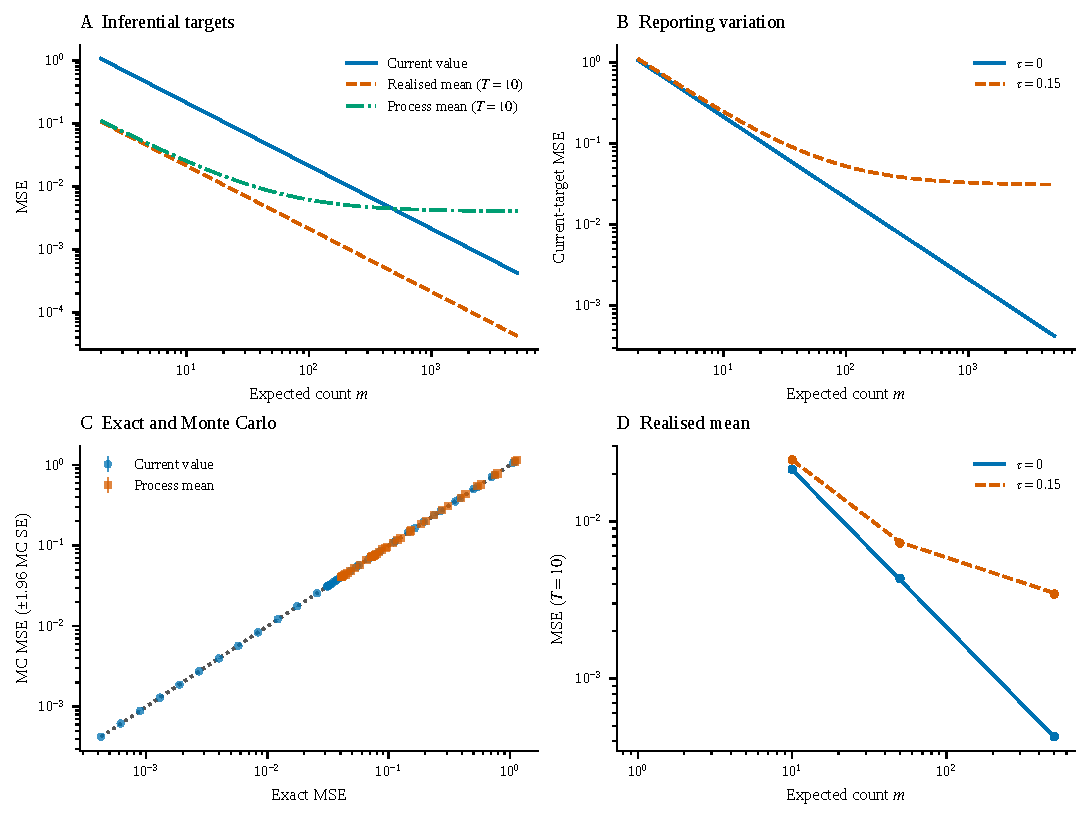
\includegraphics[width=0.92\linewidth]{figures/fig_01_targets.pdf}
\caption{Model risks for the three targets. (A) Mean squared error against expected count $m$ for the current value, the realised mean and the process mean over $T=10$ independent periods. (B) Current-value risk with fixed reporting ($\tau=0$) and with period-level reporting variation ($\tau=0.15$). (C) Exact risks against known-truth Monte Carlo estimates with 1.96 Monte Carlo standard errors. (D) Realised-mean risk over $T=10$ periods at three scales. Parameters: $\Rbar=1.15$, $v_R=0.04$, $k=0.35$, $\rho=0.25$. Counts are simulated under the fixed-exposure model, so the curves describe that model and not the hospital data.}
\label{fig:targets}
\end{figure}

\section{Reporting volatility and identification}
\label{sec:reporting}

\subsection{Period-level reporting variation}
\label{sec:reporting-volatility}

Replace H1 by a common period-specific reporting probability $p_t\in[0,1]$, independent of $R_t$ and of $n$, with known mean $\rho>0$ and $\Var(p_t)=\rho^2\tau^2$ (H5). Reporting remains independent across infections given $p_t$, so $\tau^2\le(1-\rho)/\rho$. The estimator still divides by $m=\rho n$ and does not observe $p_t$.

\begin{proposition}[Reporting volatility and second-moment nonidentification]
\label{prop:report-noise}
Under H2--H5, put $Q=\Rbar^2+v_R$. Then
\begin{equation}
  \E(\Rhat_t)=\Rbar,\qquad
  \Var(\Rhat_t)=v_R+v_H+\frac{A_H}{m},\qquad
  v_H=\tau^2Q,\qquad
  A_H=\Rbar+\frac{\rho(1+\tau^2)Q}{k}.
  \label{eq:vH-AH}
\end{equation}
For known $m$, $\rho$ and $k$, the single-period mean and variance in Eq.~\eqref{eq:vH-AH} depend on $v_R$ and $\tau^2$ only through $U=(1+\tau^2)(\Rbar^2+v_R)$.
\end{proposition}

Given $R_t$ and $p_t$ the estimator has mean $(p_t/\rho)R_t$, so a shared reporting shock is not averaged away by more infections in the same period. The statement is deliberately narrow. It concerns the first two moments of one period's count within the specified family. It does not exclude identification from full count distributions, from temporal structure under further assumptions, or from external measurements of reporting; it also assumes that reporting is independent of transmission, an assumption Section~\ref{sec:discussion} relaxes.

\begin{corollary}[Current and realised-mean risks with volatile reporting]
\label{cor:report-current}
Under H2--H5, the current-value risk is:
\begin{equation}
  \E[(\Rhat_t-R_t)^2]=v_H+\frac{A_H}{m}.
  \label{eq:vH-current}
\end{equation}
If, in addition, the $p_t$ are independent and identically distributed, independent of the transmission trajectory, and counts are independent given both trajectories, then
\begin{equation}
  \E[(\overline{\Rhat}_T-\Rbar_T)^2]=\frac{v_H+A_H/m}{T},\qquad
  \E[(\overline{\Rhat}_T-\Rbar)^2]=B_T+\frac{v_H+A_H/m}{T}.
  \label{eq:report-means}
\end{equation}
\end{corollary}

At fixed $T$, unobserved reporting volatility leaves the floor $v_H/T$ on the realised-mean target as $m$ grows, so a target free of transmission variation is not free of reporting error. The crossover scale with volatile reporting, $m_{\times,H}=A_H/(v_R+v_H)$, is never larger than $\mx$ (Eq.~\eqref{eq:mx-gap}); the lower crossover accompanies a larger risk, not better surveillance. Proofs are in Appendix~\ref{app:prop2}.

\subsection{From the branching experiment to surveillance counts}
\label{sec:reporting-scope}

If the scale $m$ is random and associated with transmission, conditional unbiasedness given $(R_t,m)$ still yields
\begin{equation}
 \E[(\Rhat_t-\Rbar)^2\mid m]
 =\frac{\E(R_t\mid m)+\rho\E(R_t^2\mid m)/k}{m}
 +\Var(R_t\mid m)+[\E(R_t\mid m)-\Rbar]^2,
\label{eq:endogenous-risk}
\end{equation}
and the conditional moments in Eq.~\eqref{eq:endogenous-risk} can change with scale. A constant intercept plus a constant coefficient on inverse count therefore does not follow when the count scale is itself an epidemic outcome, as it is in surveillance. Delays, aggregation, ratio denominators and changing conditional means further separate an apparent statistic from the experiment above. The rest of the paper accordingly treats empirical dispersion diagnostics as descriptive quantities and asks, with a known-truth audit, what they recover.

\section{Data, diagnostic and analysis plan}
\label{sec:diagnostics}

\subsection{Data and apparent reproduction number}
\label{sec:diag-data}

We used the National Healthcare Safety Network (NHSN) weekly hospital respiratory-data snapshot retrieved on 20 October 2026 and restricted influenza admissions to the 50 US states and the District of Columbia \citep{cdc2026nhsn, frutos2025evaluation}. Hospital participation varied during the series. Reporting was voluntary from May to October 2024 before it became mandatory again from 1 November 2024 \citep{cms2024reporting}, and the national Respiratory Illnesses Data Channel was not updated from 3 October to 13 November 2025 \citep{cdc2026datachannel}. The analysis describes this surveillance system and does not estimate an effect of either event. Two external sources were added for the analyses of Section~\ref{sec:diag-amend2}: state resident populations from the Census Bureau Vintage 2025 estimates \citep{census2026popest}, and the issue history of the same NHSN admission series from the Delphi Epidata archive \citep{reinhart2021open}, which records the first published and every revised value of each state-week count from November 2024 onwards.

The windows were the early-growth phases of four seasons: 1 October--26 November 2022, 7 October--23 December 2023, 9 November--28 December 2024 and 4 October--27 December 2025. Each is the contiguous national segment with weekly growth of at least 1.05 before the first turning point after the season's admissible start; the 2024 start follows the return to mandatory reporting. The rule is applied identically to every season, and inference conditions on the selected windows. Sensitivity analyses use growth thresholds of 1.02 and 1.10 and fixed calendar windows for the first three seasons (8 October--26 November 2022, 14 October--16 December 2023 and 9 November 2024--18 January 2025). Missing or suppressed counts were kept missing rather than set to zero.

With $C_t$ the admissions in week $t$, the apparent reproduction number of a state-week is the growth-to-reproduction transform:
\begin{equation}
R_{A,t}=[\max\{0,\,1+(\theta/7)\log\{(C_{t+1}+0.5)/(C_t+0.5)\}\}]^{\alpha},\qquad
\alpha=(g_\mu/g_\sigma)^2,\quad\theta=g_\sigma^2/g_\mu.
\label{eq:ra}
\end{equation}
The transform follows the renewal relation between growth rate and reproduction number for a gamma-distributed interval \citep{wallinga2007how}. It is not a true reproduction number or a posterior estimate from a renewal model \citep{cori2013new, eales2024differences}. A row requires observed counts in weeks $t$ and $t+1$ and $C_t\ge5$, which leaves 1,748 state-weeks from 51 jurisdictions and 42 calendar weeks. The rows contain 1,969 distinct state-week counts in 210 runs of consecutive weeks.

The primary interval has mean $g_\mu=3.6$ days and standard deviation $g_\sigma=1.6$ days, the household serial-interval estimate of \citet{cowling2009estimation}. That estimate is a Weibull fit to 14 household transmission pairs; Eq.~\eqref{eq:ra} uses the gamma distribution with the same mean and standard deviation. A serial interval is not a generation interval \citep{vink2014serial}. Sensitivity analyses set the mean to 3.2 and 4.0 days and the standard deviation to 1.2 and 2.0 days; the lower mean is close to the intrinsic generation-time estimate from US household data \citep{chan2025estimating}.

\subsection{The diagnostic and its three summaries}
\label{sec:diag-definition}

For the apparent statistic $X=R_A$ with pooled mean $\bar X$, the relative squared deviation and its affine working model are:
\begin{equation}
L_{st}=\frac{(X_{st}-\bar X)^2}{\bar X^2},
\qquad \E(L_{st}\mid C_{st})=a+\frac{b}{C_{st}}.
\label{eq:affine}
\end{equation}
This is the empirical counterpart of $V(m)/\Rbar^2$ in Eq.~\eqref{eq:var-average}, with a realised count in place of the expected scale and an apparent statistic in place of $\Rhat_t$. It has the form of the additive overdispersion model of funnel plots \citep{spiegelhalter2005funnel, spiegelhalter2012statistical}. Three summaries of the fit follow.

The intercept $a$ is the count-independent relative dispersion: all relative variation in $X$ that does not scale with count. When reporting probabilities do not vary from week to week ($\tau=0$), $a$ estimates the relative variance of transmission, $\tilde v_R=v_R/\Rbar^2$. When reporting shocks vary between weeks, $a$ estimates $\tilde v_R+\tilde v_H$, where $\tilde v_H$ is the relative variance that the shocks induce in the ratio statistic (Appendix~\ref{app:ratio-shocks}). A reporting level that is constant over consecutive weeks cancels in the ratio, as it does in renewal estimators \citep{cori2013new, gostic2020practical}. By Proposition~\ref{prop:report-noise}, single-period cross-sectional moments cannot separate the two components. The estimator also need not weight them equally: when the shocks are drawn independently for each state-week, the fitted intercept recovers only part of $\tilde v_H$, and Section~\ref{sec:res-bias} quantifies the shortfall. The intercept is therefore read throughout as reflecting transmission and reporting variation, not as an estimate of their sum. It is also not an error floor for the current value: with $\tau=0$ that floor is zero, and with $\tau>0$ it is $\tilde v_H$. For the process mean, $a$ approximates the relative error that more cases cannot remove, to the extent that the affine form holds (Section~\ref{sec:res-form}).

The counting slope $b$ is read against two references. A delta expansion of Eq.~\eqref{eq:ra} under independent Poisson counts in consecutive weeks gives the independent-Poisson reference
$\bP=\overline{\kappa(g)^2[1+(C_t+0.5)/(C_{t+1}+0.5)]}$, a mean over rows, with $\kappa(g)=(g_\mu/7)/[1+\theta\log(g)/7]$ and $g=(C_{t+1}+0.5)/(C_t+0.5)$. Each row is evaluated at its own growth factor and normalised by $\bar X^2$, which approximates the expansion around $\bar X$ when the row's $R_A$ is close to $\bar X$; $\bP$ is therefore a plug-in normalisation, not an exact expectation. For the primary sample $\bP=0.4455$. Two alternatives show how much the normalisation matters. Replacing the unit normalisation by each row's ratio $X_{st}/\bar X$ gives 0.4199. The slope fitted to panels of independent Poisson counts drawn around the observed means, with the same transform, row filter and fit, gives 0.3977 (Table~\ref{tab:r2-poisson}). The term 1 is the Poisson variance of the denominator count. In a branching chain the denominator week contains the parents of the numerator week, so conditioning on the realised parents leaves only the binomial reporting part of that variance, $(1-\rho)/C_t$. With Poisson offspring and reporting probability $\rho$ this gives the branching-Poisson reference and its ratio to $\bP$:
\begin{equation}
b_{\mathrm{P,br}}(\rho)=\overline{\kappa(g)^2[(1-\rho)+(C_t+0.5)/(C_{t+1}+0.5)]},\qquad
r(\rho)=\frac{b_{\mathrm{P,br}}(\rho)}{\bP}\approx\frac{1+(1-\rho)g}{1+g}=1-\frac{\rho g}{1+g}.
\label{eq:branching-reference}
\end{equation}
Averaged over the observed rows, $r(\rho)$ is 0.944, 0.861, 0.722 and 0.443 for $\rho=0.1$, 0.25, 0.5 and 1 (Table~\ref{tab:ma_baselines}). The observed-denominator model of Section~\ref{sec:model-observed} has the structure of the branching-Poisson reference, and the known-scale estimator of Section~\ref{sec:model-branching} is its limit without denominator noise. The ratio $b/\bP$ asks whether counting variation exceeds independent-Poisson noise; $b/b_{\mathrm{P,br}}(\rho)$ asks the same for a branching chain, at a reporting probability that the data do not identify.

The third summary is the crossover count $b/a$, at which the fitted counting term equals the count-independent term. It is the empirical analogue of $\mx$ in admissions per week; $\mx$ refers to the expected count of a branching experiment. At $C=b/a$ a shrinkage estimator of the Fay--Herriot type places half its weight on the direct estimate (Eq.~\eqref{eq:shrink-weight}). Table~\ref{tab:rosetta} lists the conditions under which each summary identifies its theoretical counterpart and the direction of distortion when they fail.

\begin{table}[!tbp]
\centering
\scriptsize
\setlength{\tabcolsep}{3pt}
\caption{Mapping from theoretical inferential targets to empirical surveillance diagnostics}
\label{tab:rosetta}
\begin{tabularx}{\linewidth}{@{}p{0.20\linewidth}p{0.18\linewidth}p{0.28\linewidth}p{0.28\linewidth}@{}}
\toprule
Theoretical Target (Section~\ref{sec:model}) & Empirical Diagnostic (Section~\ref{sec:diagnostics}) & Exact Equivalence Conditions & Distortion Mechanism and Bias Direction \\
\midrule
Relative transmission variance: $\tilde v_R = v_R / \Rbar^2$ & Dispersion Intercept: $a$ & Constant reporting probability ($\tau = 0$); scale-independent transmission ($\gamma = 0$). & If reporting varies ($\tau > 0$), $a \approx \tilde v_R + \tilde v_H$. The intercept is an upper bound on $\tilde v_R$, not an error floor. Under scale dependence ($\gamma > 0$), $a < \tilde v_R$. \\
\addlinespace[2pt]
Counting error scale: $\tilde A = A / \Rbar^2$ & Counting Slope: $b$ & Independent Poisson limit ($\rho \to 0$ gives $b \approx \bP$); branching Poisson ($b \approx b_{\mathrm{P,br}}(\rho)$). & Inflated by offspring overdispersion ($k < \infty$, $b > b_{\mathrm{P,br}}$) or unmodelled scale-dependent heterogeneity ($\gamma > 0$). \\
\addlinespace[2pt]
Crossover scale: $\mx = A / v_R$ & Crossover Count: $b/a$ & Exact match between $A$ and $b$, and between $v_R$ and $a$. & Under reporting shocks ($\tau > 0$), $b/a$ is attenuated below $\mx$; under scale dependence ($\gamma > 0$), $b/a$ is inflated. $b/a$ is an in-sample balance point. \\
\bottomrule
\end{tabularx}
\par\smallskip
\begin{minipage}{\linewidth}\footnotesize\raggedright Formal correspondence between the theoretical parameters derived under the branching model in Section~\ref{sec:model} and the empirical summaries estimated by the cross-sectional dispersion diagnostic in Section~\ref{sec:diagnostics}. The table makes explicit the conditions under which empirical diagnostics identify theoretical quantities and the sign of the distortion when those conditions fail.\end{minipage}
\end{table}


\subsection{Estimation and inference}
\label{sec:diag-estimation}

The affine mean was fitted by iterated feasible generalised least squares with weights inversely proportional to the squared fitted mean, which minimises a gamma quasi-deviance; this is an estimating criterion, not a distributional claim. The primary interval is the two-way cluster-robust sandwich of \citet{cameron2011robust} for the stacked estimating equations of $\bar X$ and the affine fit, clustered by state and calendar week, with small-sample factors $G/(G-1)$ and critical values from the $t$ distribution on 41 degrees of freedom, one fewer than the number of weeks. The interval for $b/a$ is formed on the log scale. Two resampling checks accompany it: a calendar-week block bootstrap (1,999 draws) that resamples whole weeks with all their state rows, and a wild cluster bootstrap-$t$ over calendar weeks with six-point weights and the null $a=0$ imposed (9,999 draws) \citep{cameron2008bootstrap, webb2023reworking}. In the wild bootstrap, losses at or below $10^{-7}$ in a bootstrap sample are set to $10^{-7}$ before the restricted fit; this affected 13.5\% of bootstrap rows, and Table~\ref{tab:r2-clamp} reports the test under other thresholds and without the clamp. The state-by-week pigeonhole bootstrap \citep{owen2007pigeonhole} used for the supplementary analyses is conservative on this design: under the fresh-draw generators of Section~\ref{sec:diag-sim} its standard deviation of $\hat a$ was 1.55--1.78 times the Monte Carlo standard deviation (Table~\ref{tab:r2-bootstrap-sd}). Every interval quoted in the text is listed with its type and source in Table~\ref{tab:r2-interval-types}; all are 95\% intervals, and an interval without a stated type has the type of the nearest preceding interval of the same paragraph.

\subsection{Analysis plan and primary test}
\label{sec:diag-plan}

The analysis plan was written after an exploratory analysis of the same data, and it lists the estimates and the season-test $p$ values that were then known, so that each choice can be judged against them. It was fixed, with a checksum, before any analysis in Section~\ref{sec:results} was run. Because the data had been seen, the plan does not make the primary test confirmatory in the sense of an untouched hypothesis; what it fixes is the robustness rule for the intercept, the primary calibration of the season test and the obligation to report every specified analysis. The data vintage, the sample and $R_A$ with the primary interval were frozen.

The primary test (E1) is of $H_0\colon a=0$ against a two-sided alternative at $\alpha=0.05$, tested with the two-way sandwich $t$ statistic on 41 degrees of freedom. The claim that count-independent dispersion remains is called robust only if the primary test rejects and the 95\% lower limit of $a$ stays above zero in each of nine sensitivity analyses. Two vary the generation-interval mean (S-a1) and standard deviation (S-a2). Three change the row filters: count floors of 10, 20 and 50 (S-a3), the fixed calendar windows (S-a4) and growth thresholds (S-a5). Three remove data: transitions that touch the 2025 data-channel interruption (S-a6), one season at a time (S-a7) and rows with hospital reporting coverage below 90\% in either week (S-a8). The last (S-a9) removes one calendar week at a time to measure influence.

A within-week intercept (E3) is a different estimand, not a sensitivity analysis. It replaces $\bar X$ by the mean of the same calendar week computed without the row's own state, which removes common national variation by week; the week mean including the own row and a version that also rescales by the week mean are reported as alternatives. Its interval is the calendar-week block bootstrap.

The secondary test asks whether season intercepts differ. In a model with four season intercepts $a_s$ and a common slope, $H_0\colon\log a_1=\dots=\log a_4$ is tested with the Wald statistic $W_{\mathrm{CGM}}$ that uses the two-way sandwich covariance. The season label is constant within a calendar week, so it is assigned at the level of 42 weeks in four groups. With few clusters at the level of assignment, wild cluster bootstrap tests can be badly mis-sized and randomisation inference at that level is recommended \citep{mackinnon2018wild, mackinnon2023cluster}. The primary reference distribution is therefore a permutation of season labels across calendar weeks that keeps the number of weeks per season (9,999 permutations); it assumes exchangeable weeks and ignores serial dependence between adjacent weeks. The season difference is called significant only if this $p<0.05$, whatever the other calibrations show. All other calibrations are reported, and Holm-adjusted $p$ values over E1 and the season test are given. Season intercepts are interpreted only as reflecting transmission and reporting variation together (Proposition~\ref{prop:report-noise}).

The counting slope $b/\bP$, the crossover count and the predicted relative squared error $a+b/C$ at $C=10$, 37, 100 and 1,000 were specified for estimation, without tests.

\subsection{Simulation checks}
\label{sec:diag-sim}

The conversion of $a$ into a transmission standard deviation needs a mechanism. For a simulated mechanism with recovery ratio $r=\E(\hat a)/\tilde v_R$, the implied relative standard deviation of the reproduction number is $(a/r)^{1/2}$. Its interval combines the two-way interval of $a$ with the Monte Carlo 2.5--97.5\% range of $r$. The plan required that this quantity be reported as a grid over mechanisms and never as a single estimate, and that $a^{1/2}$ be described as a relative standard deviation of transmission and reporting variation combined, not of transmission alone. A mechanism reproduces the counting slope when its Monte Carlo 2.5--97.5\% range of $b/\bP$ contains the observed value. Synthetic panels are generated on the exact design of the data. The expected count level is calibrated to the observed median retained count of 45, and the heterogeneity amplitude is calibrated so that the mean fitted intercept equals the observed $a$ (Appendix~\ref{app:audit}). Five checks with fixed criteria were specified:
\begin{itemize}
\item SC1, two generations per week: a daily renewal process with the primary generation interval, Poisson or negative binomial ($k=0.3$) offspring and weekly binomial reporting at $\rho\in\{0.003,0.01,0.1\}$. The one-generation recovery map carries over if $\E(\hat a)/v_R$ lies in $[0.8,1.25]$ in every cell.
\item SC2 and SC3, reporting and offspring dispersion: a grid of $\rho\in\{0.001,0.003,0.01,0.03,0.1,0.25,0.5,1\}$ and $k\in\{0.1,0.3,1,3,\infty\}$ with independent transmission heterogeneity, 100 panels per cell. SC2 requires intercept recovery in $[0.9,1.1]$ in every cell; SC3 requires the mean of $b/\bP$ to lie in $[0.9,1.1]$ in every cell with $\rho\le0.01$. The range $\rho=0.001$--0.01 for the probability that an infection becomes a reported admission is assumed from burden estimates \citep{reed2015estimating, hayward2014comparative}, not estimated.
\item SC4 and SC5, interval validity: these use generators that redraw the heterogeneity field in every replicate. FD-S1 has independent heterogeneity, and FD-S8 has scale-dependent heterogeneity with state-week reporting shocks. FD-S9 adds to FD-S8 a national calendar-week share of 0.25, 0.5 or 0.75 of the heterogeneity; this family was defined after the data had been seen. SC4 requires coverage of $\E(\hat a)$ by the two-way interval of at least 0.90 under every generator. SC5 calls the gap between the observed standard error of $a$ and the generators' Monte Carlo standard deviation explained if their ratio lies in $[0.67,1.5]$ for at least one generator.
\end{itemize}

\subsection{Amendments and additional analyses}
\label{sec:diag-amend2}

The plan was amended twice, and both amendments are distributed with it. Amendment 1 recorded implementation details that the plan had left open: seeds, the restricted fit and loss clamp of the wild bootstrap, and the construction of the daily-renewal generator. It stated that these details were fixed before the full runs, but the run logs show that the full runs of the primary test, the season test and the simulation checks had finished before it was written. The details were already in the code used for those runs, and no evidence was found that any of them was changed after a result was seen. The season script was edited once after its first full run. The text of that edit could not be recovered, but every quantity logged by both runs is identical, including the primary permutation $p$ value, the other calibrations, the data sensitivities and the power analysis.

Amendment 2 was fixed, with a checksum, before any of the following analyses was run. Each is secondary or descriptive, none can change the verdict of the primary test, the significance level, the calibration or the data, and each was specified with its reading rule.
\begin{itemize}
\item Functional form. The observed mean loss in each decile of $C_t$, with a calendar-week block-bootstrap interval, is compared with the affine fit, a power law $cC^{-\gamma}$ and a three-parameter model $a+bC^{-\gamma}$. The intercept is said to survive a free exponent if the block-bootstrap interval of $a$ in the three-parameter model excludes zero; $\gamma=1$ is called compatible with the data if its interval contains one.
\item Model-free floor. Among rows with $C_t$ at or above the 75th, 90th and 95th percentiles, the mean loss minus the mean counting term, with either $\hat b$ or $\bP$ as the slope, estimates the count-independent component without extrapolation.
\item Population size. The intercept is made linear in the standardised log population $z$ of the jurisdiction, $a_0+a_1z$, with a common slope, and $a_1=0$ is tested with the two-way sandwich on 41 degrees of freedom. If the interval of $a_1$ lies below zero, statements about what more cases buy are restricted to jurisdictions of comparable size and the error at a given count is reported by population tertile. A log-link intercept, a slope that also varies with $z$, and separate fits by tertile are secondary.
\item Bias of the intercept. Under the fresh-draw generators with reporting shocks, and in a sweep of the transmission share of their variance (1, 0.75, 0.25), the relative bias $\E(\hat a)/(\tilde v_R+\tilde v_H)-1$ and the weight $w_H$ that solves $\E(\hat a)=\tilde v_R+w_H\tilde v_H$ are estimated. If every bias interval excludes zero, $\hat a$ is described as reflecting, not estimating, the total.
\item Generator realism. Six cells of a state-realistic generator anchor transmission to the smoothed observed epidemic curve, scale its variance by state and allow clustered admissions. Four tests compare the Monte Carlo range of each cell with the data: the slope ratio $b/\bP$ (T1), the 90th percentile of $C_t$ (T2), the ratio of pooled to within-state slope (T3) and the between-state coefficient of variation of the intercepts (T4). The generators reproduce the data if all four pass in one cell. Their design used the observed slope and between-state dispersion, and no inferential result rests on them.
\item Reporting data. The fit is repeated with counts scaled by the share of hospitals reporting in each state-week, and on the first-issue and latest-issue counts of the archive for the 661 rows whose first issue is provisional.
\item Calibration details. The wild bootstrap is repeated under four loss clamps and without one; the standard deviation of the pigeonhole bootstrap is compared with the Monte Carlo standard deviation of $\hat a$ (it is called conservative only if the ratio exceeds one under every fresh-draw generator); and $b/\bP$ is reported under the three Poisson references.
\end{itemize}

\section{Results for US influenza hospital admissions}
\label{sec:results}

\subsection{A count-independent floor}
\label{sec:res-floor}

The pooled affine fit of Eq.~\eqref{eq:affine} gave $a=0.0150$ (two-way 95\% CI 0.0109--0.0191; $t_{41}=7.36$, two-sided $p=5.1\times10^{-9}$) and $b=0.560$ (0.430--0.690) (Table~\ref{tab:rev_intercept}). The primary test (E1) rejects $a=0$, and the Holm-adjusted $p$ over the two tests of the plan is $1.0\times10^{-8}$. The secondary calibrations agree. Clustering by state alone or by week alone gave intervals of 0.0125--0.0174 and 0.0112--0.0188. The week-cluster wild bootstrap-$t$ with the null imposed gave $p=0.0001$, the smallest value attainable with 9,999 draws, at every clamp of the bootstrap losses from $10^{-9}$ to $10^{-3}$ and 0.0003 without a clamp (Table~\ref{tab:r2-clamp}). None of the 1,999 calendar-week block-bootstrap draws gave $a\le0$ (block-bootstrap percentile interval 0.0107--0.0192).

The lower limit of $a$ stayed above zero in every sensitivity analysis of the plan, so the claim meets the robustness rule (Fig.~\ref{fig:rev-intercept}). Point estimates ranged from 0.0117 to 0.0202 over 16 independent specifications, and the smallest lower limit, 0.0082, came from leaving out the 2025--26 season. The generation interval moved $a$ most: a mean of 3.2 days gave 0.0117 and a mean of 4.0 days gave 0.0186, because the transform~\eqref{eq:ra} rescales all deviations together. Raising the count floor lowered $a$ slightly, to 0.0130 (0.0088--0.0172) at $C_t\ge50$ on 828 rows. The fixed calendar windows gave the widest interval, 0.0092--0.0311, on 1,263 rows from three seasons. Leaving out one calendar week at a time gave estimates of 0.0136--0.0156 with a smallest lower limit of 0.0100. Count-independent dispersion is therefore present in these data under every specification that the plan fixed, provided the decline with count is inverse; Section~\ref{sec:res-form} examines that proviso.

\begin{table}[!tbp]
\centering
\scriptsize
\setlength{\tabcolsep}{3pt}
\caption{Count-independent intercept $a$: primary test of the analysis plan, secondary calibrations and sensitivity analyses}
\label{tab:rev_intercept}
\begin{tabularx}{\linewidth}{@{}l*{6}{>{\centering\arraybackslash}X}@{}}
\toprule
Analysis (rows) & $a$ & 95\% CI & $t$ & $p$ (two-sided) & $b/a$ & $b/b_P$ \\
\midrule
\multicolumn{7}{l}{\emph{E1, primary: two-way CGM sandwich, $t_{41}$}} \\
All rows (1748) & 0.0150 & 0.0109--0.0191 & 7.36 & $<10^{-4}$ & 37.4 & 1.257 \\
State-cluster sandwich & 0.0150 & 0.0125--0.0174 & 12.23 & $<10^{-4}$ & -- & -- \\
Week-cluster sandwich & 0.0150 & 0.0112--0.0188 & 7.94 & $<10^{-4}$ & -- & -- \\
Week wild bootstrap-$t$, $a=0$ imposed ($B$=9,999) & -- & -- & -- & 0.0001 & -- & -- \\
Calendar-week block bootstrap ($B$=1,999) & -- & 0.0107--0.0192 & -- & -- & 23.4--60.5 & 0.97--1.59 \\
\midrule
\multicolumn{7}{l}{\emph{Sensitivity analyses (two-way sandwich)}} \\
S-a1 GI mean 3.2 (1748) & 0.0117 & 0.0085--0.0149 & 7.44 & $<10^{-4}$ & 37.6 & 1.259 \\
S-a1 GI mean 4.0 (1748) & 0.0186 & 0.0134--0.0237 & 7.27 & $<10^{-4}$ & 37.5 & 1.259 \\
S-a2 GI SD 1.2 (1748) & 0.0154 & 0.0111--0.0197 & 7.27 & $<10^{-4}$ & 37.6 & 1.278 \\
S-a2 GI SD 2.0 (1748) & 0.0144 & 0.0105--0.0183 & 7.46 & $<10^{-4}$ & 37.4 & 1.234 \\
S-a3 count floor 10 (1600) & 0.0140 & 0.0100--0.0180 & 7.07 & $<10^{-4}$ & 46.1 & 1.461 \\
S-a3 count floor 20 (1268) & 0.0136 & 0.0096--0.0176 & 6.82 & $<10^{-4}$ & 48.6 & 1.529 \\
S-a3 count floor 50 (828) & 0.0130 & 0.0088--0.0172 & 6.21 & $<10^{-4}$ & 51.5 & 1.591 \\
S-a4 calendar windows (1263) & 0.0202 & 0.0092--0.0311 & 3.78 & 0.0008 & 25.6 & 1.140 \\
S-a5 threshold 1.02 (1748) & 0.0150 & 0.0109--0.0191 & 7.36 & $<10^{-4}$ & 37.4 & 1.257 \\
S-a5 threshold 1.1 (1564) & 0.0141 & 0.0105--0.0176 & 8.00 & $<10^{-4}$ & 38.6 & 1.255 \\
S-a6 exclude pause (1554) & 0.0139 & 0.0103--0.0176 & 7.76 & $<10^{-4}$ & 41.5 & 1.331 \\
S-a7 drop 2022-23 (1383) & 0.0160 & 0.0105--0.0214 & 5.97 & $<10^{-4}$ & 31.0 & 1.101 \\
S-a7 drop 2023-24 (1249) & 0.0163 & 0.0122--0.0204 & 8.08 & $<10^{-4}$ & 33.3 & 1.240 \\
S-a7 drop 2024-25 (1392) & 0.0152 & 0.0100--0.0204 & 5.89 & $<10^{-4}$ & 36.6 & 1.230 \\
S-a7 drop 2025-26 (1220) & 0.0119 & 0.0082--0.0156 & 6.57 & $<10^{-4}$ & 55.5 & 1.488 \\
S-a8 coverage $\ge$ 90\% (1358) & 0.0159 & 0.0110--0.0207 & 6.59 & $<10^{-4}$ & 31.0 & 1.104 \\
S-a9 leave one week out (42 fits) & 0.0136--0.0156 & min lower 0.0100 & -- & max $<10^{-4}$ & -- & 1.188--1.306 \\
\bottomrule
\end{tabularx}
\par\smallskip\parbox{\linewidth}{\scriptsize\linespread{1.15}\selectfont Robustness rule (locked analysis plan): verdict \emph{robust}; analyses with a lower limit $\le 0$: none. S-a5 with threshold 1.02 reproduces the primary windows. Block-bootstrap columns give percentile intervals.}
\end{table}


\begin{figure}[!tbp]
\centering
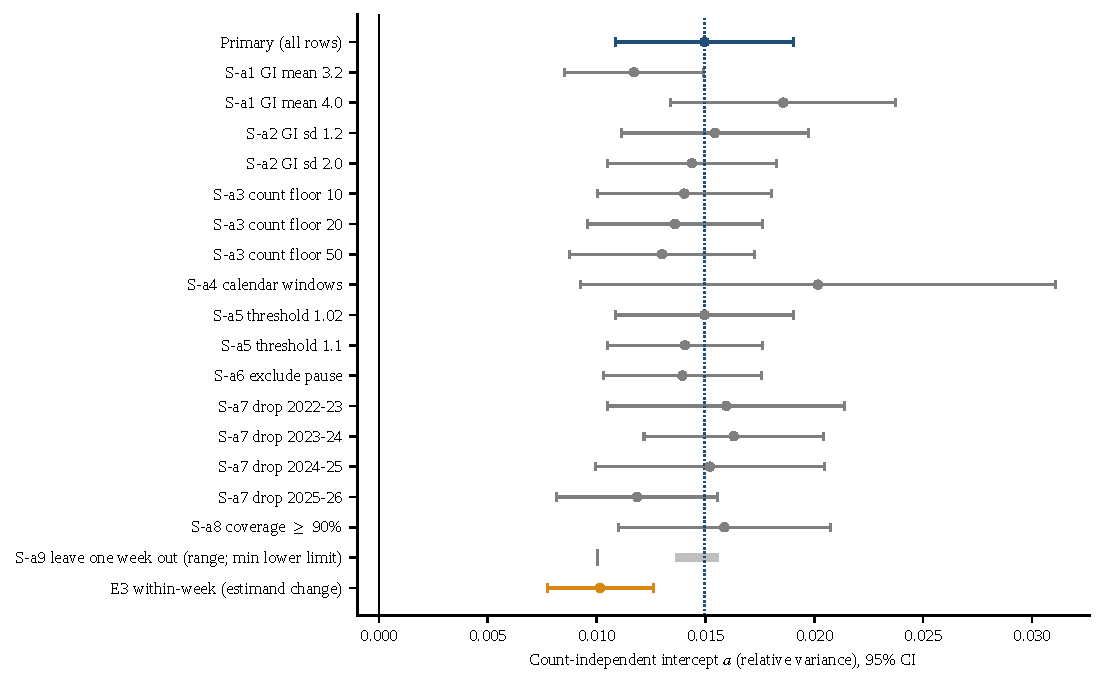
\includegraphics[width=0.92\linewidth]{figures/fig_02_fig_rev_intercept_sens.pdf}
\caption{Count-independent intercept $a$ of the affine dispersion model for $R_A$ under the primary analysis (E1) and sensitivity analyses S-a1 to S-a9, with two-way cluster-robust 95\% confidence intervals. The dotted line marks the primary estimate and the solid line marks zero. For S-a9 the grey bar spans the 42 leave-one-week-out point estimates and the tick marks their smallest lower limit. The within-week intercept (E3, block-bootstrap interval) is a different estimand and is shown for comparison.}
\label{fig:rev-intercept}
\end{figure}

\subsection{How well the affine form fits}
\label{sec:res-form}

The affine form describes the decline of the loss with count only approximately (Table~\ref{tab:r2-deciles}; Fig.~\ref{fig:r2-deciles}). Across deciles of the current-week count the mean loss fell from 0.0684 to 0.0110, and the affine prediction lay outside the block-bootstrap interval of the observed mean in three of ten deciles: above it in the lowest decile (0.0906 against 0.0538--0.0854) and in the highest (0.0158 against 0.0079--0.0137), and below it in the fifth (0.0296 against 0.0310--0.0501). A fit $a+bC^{-\gamma}$ with a free exponent lowered the quasi-deviance by 10.67, and the gain exceeded 2 in 94.6\% of calendar-week block-bootstrap draws (Table~\ref{tab:r2-floor}). Its exponent was $\gamma=0.617$ (week bootstrap 0.355--0.870; state bootstrap 0.438--0.862), so the inverse-count decline $\gamma=1$ lies outside both intervals. Its intercept was 0.0089, and the week-bootstrap interval reached zero ($-0.0014$ to 0.0137; 4.0\% of draws at or below zero), whereas the state-bootstrap interval did not (0.0034--0.0144). Under the reading rule fixed in Amendment~2 the floor therefore does not survive a free exponent. Within the observed counts a slower decline with a smaller constant and an inverse decline with a larger constant describe the data almost equally well, and the intercept of either model is an extrapolation beyond the largest counts.

The rows with the largest counts give the floor without a model for the decline (Table~\ref{tab:r2-floor}; Fig.~\ref{fig:r2-floor}). Among the 175 state-weeks at or above the 90th percentile of the count ($C_t\ge389$, mean 882) the mean loss was 0.0110 (week bootstrap 0.0078--0.0139), a relative root mean squared deviation of 10.5\% (8.8--11.8\%). Subtracting the counting term with the fitted slope left 0.0102 (0.0069--0.0132), a relative standard deviation of 10.1\% (8.3--11.5\%), and subtracting it with the Poisson reference left 0.0104 (0.0071--0.0132). At the 75th and 95th percentiles the net relative standard deviation was 11.8\% (9.8--13.2\%) and 9.8\% (8.0--11.1\%). At the largest observed counts, therefore, a count-independent relative error of about 10\% remains, and all of these intervals exclude zero. The model-free value at the 90th percentile lies between the three-parameter intercept and the affine one.

\begin{figure}[!tbp]
\centering
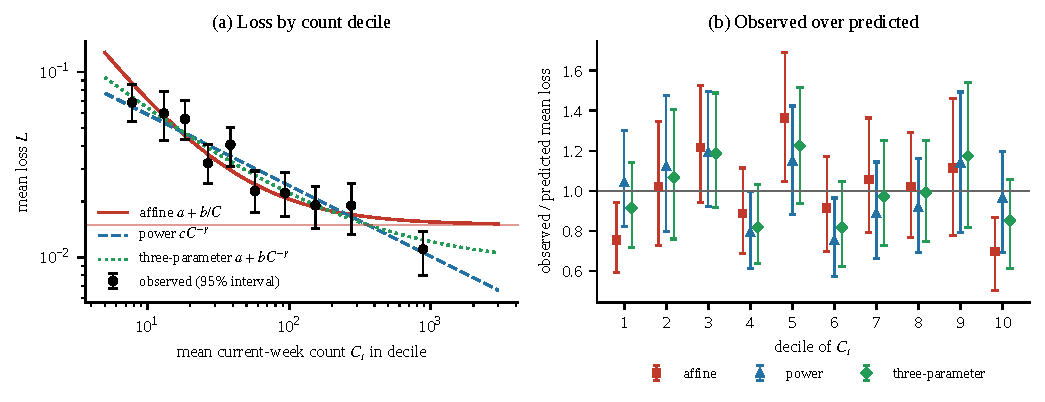
\includegraphics[width=0.98\linewidth]{figures/fig_03_deciles.pdf}
\caption{Loss by decile of the current-week count. (A) Mean relative squared deviation $L$ against mean count $C_t$ on log scales, with calendar-week block-bootstrap 95\% intervals (1,999 draws). Lines show the fitted affine ($a+b/C$), power ($cC^{-\gamma}$) and three-parameter ($a+bC^{-\gamma}$) curves. (B) Ratio of the observed mean loss to the prediction of each model by decile; the dotted line marks 1.}
\label{fig:r2-deciles}
\end{figure}

\begin{table}[!tbp]
\centering
\scriptsize\renewcommand{\arraystretch}{1.15}
\setlength{\tabcolsep}{3pt}
\caption{The floor under a free exponent and without a model}
\label{tab:r2-floor}
\begin{tabularx}{\linewidth}{@{}Xrll@{}}
\toprule
Quantity & Estimate & Week bootstrap & State bootstrap \\
\midrule
\multicolumn{4}{@{}l}{\textit{Affine fit $a+b/C$ (primary, for reference)}} \\
$a$ (two-way interval) & 0.0150 & 0.0109--0.0191 & -- \\
\midrule
\multicolumn{4}{@{}l}{\textit{Three-parameter fit $a+bC^{-\gamma}$}} \\
$a$ & 0.0089 & $-$0.0014 to 0.0137 & 0.0034--0.0144 \\
$b$ & 0.228 & 0.130--0.436 & -- \\
$\gamma$ & 0.617 & 0.355--0.870 & 0.438--0.862 \\
Share of draws with $a\le 0$ & -- & 0.040 & 0.006 \\
Quasi-deviance gain over affine & 10.67 & share $>2$: 0.946 & -- \\
\midrule
\multicolumn{4}{@{}l}{\textit{Model-free floor among rows with $C_t$ at or above a quantile}} \\
P75 ($C_t\ge 152$, $n=438$, mean $C_t$ 497): mean $L$ & 0.0157 & 0.0117--0.0191 & -- \\
\quad mean $L-\hat b/C_t$ & 0.0139 & 0.0096--0.0176 & -- \\
\quad mean $L-b_P/C_t$ & 0.0142 & 0.0102--0.0177 & -- \\
\quad relative SD $(L-\hat b/C_t)^{1/2}$ (\%) & 11.8 & 9.8--13.2 & -- \\
P90 ($C_t\ge 389$, $n=175$, mean $C_t$ 882): mean $L$ & 0.0110 & 0.0078--0.0139 & -- \\
\quad mean $L-\hat b/C_t$ & 0.0102 & 0.0069--0.0132 & -- \\
\quad mean $L-b_P/C_t$ & 0.0104 & 0.0071--0.0132 & -- \\
\quad relative SD $(L-\hat b/C_t)^{1/2}$ (\%) & 10.1 & 8.3--11.5 & -- \\
P95 ($C_t\ge 699$, $n=90$, mean $C_t$ 1238): mean $L$ & 0.0101 & 0.0071--0.0128 & -- \\
\quad mean $L-\hat b/C_t$ & 0.0096 & 0.0064--0.0123 & -- \\
\quad mean $L-b_P/C_t$ & 0.0097 & 0.0066--0.0124 & -- \\
\quad relative SD $(L-\hat b/C_t)^{1/2}$ (\%) & 9.8 & 8.0--11.1 & -- \\
\bottomrule
\end{tabularx}
\par\smallskip\parbox{\linewidth}{\scriptsize\linespread{1.15}\selectfont Week bootstrap: calendar-week blocks (1,999 draws); state bootstrap: states resampled (999 draws). Model-free floor: mean loss of the rows above the threshold minus the mean counting term, with $\hat b$ the fitted slope or $b_P$ the Poisson reference; intervals from the calendar-week block bootstrap with $\hat b$ refitted in each draw. Reading rule of Amendment 2: the floor survives a free exponent if the week-bootstrap interval of $a$ excludes 0 (here: no).}
\end{table}


\begin{figure}[!tbp]
\centering
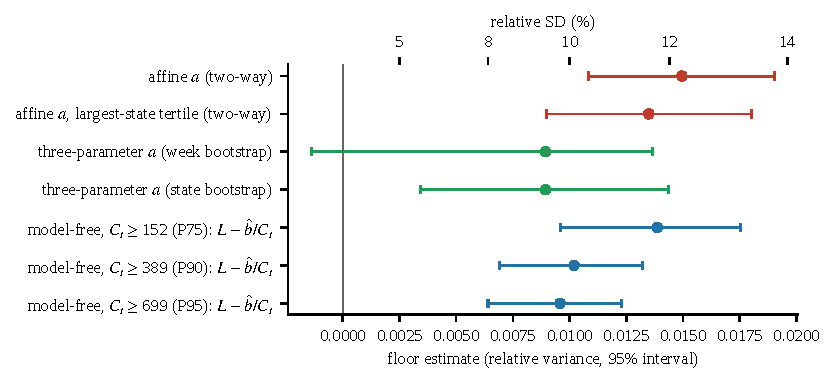
\includegraphics[width=0.92\linewidth]{figures/fig_04_floor.pdf}
\caption{Estimates of the count-independent component on the relative-variance scale, with the corresponding relative standard deviation on the upper axis. Rows show the affine intercept (two-way cluster-robust 95\% interval), the same intercept in the largest-population tertile (two-way interval) and the three-parameter intercept with calendar-week and state bootstrap 95\% intervals. The remaining rows show the model-free floor (mean loss minus the fitted counting term) among rows at or above the 75th, 90th and 95th percentiles of the count, with calendar-week block-bootstrap 95\% intervals. The solid line marks zero.}
\label{fig:r2-floor}
\end{figure}

\subsection{What more cases buy}
\label{sec:res-buy}

The observed relative error fell with count but levelled off at large counts (Table~\ref{tab:r2-deciles}). The relative root mean squared deviation of $R_A$ was 26.2\% in the lowest count decile (mean 7.8 admissions a week), 20.1\% in the fifth (mean 38.5), 14.9\% in the seventh (mean 93.5) and 10.5\% in the highest (mean 882). A ninefold increase in the mean count from the seventh to the tenth decile thus lowered the relative error by about four percentage points. The affine model gives smooth values over the same range, 26.6\% at 10 admissions, 17.3\% at 37 and 14.3\% at 100 (Table~\ref{tab:rev_error_components}). Its extrapolation to 1,000 admissions, 12.5\%, exceeds the observed relative error of the highest decile, so statements about large counts here rest on the model-free floor of Section~\ref{sec:res-form}. The crossover count, at which the two affine terms are equal, was $b/a=37.4$ admissions a week (two-way 24.1--58.3; block bootstrap 23.4--60.5). It rose to 46.1, 48.6 and 51.5 at count floors of 10, 20 and 50 and lay between 25.6 and 55.5 across the other sensitivity analyses, so its order of magnitude, a few tens of weekly admissions, is stable while its value is not. It is an in-sample balance point for this panel, not a sample-size rule for surveillance.

These values pool jurisdictions whose count-independent component differs (Section~\ref{sec:res-pop}). Separate affine fits by population tertile gave predicted relative errors at 37, 100 and 390 admissions of 18.3, 15.6 and 14.2\% in the smallest-population tertile, 17.9, 15.5 and 14.4\% in the middle tertile and 16.2, 13.5 and 12.1\% in the largest. What additional cases buy should be judged against the component of the jurisdiction concerned.

\begin{table}[!tbp]
\centering
\scriptsize
\setlength{\tabcolsep}{3pt}
\caption{What more cases buy: predicted relative squared error $a+b/C$ by count, crossover, and the within-week intercept}
\label{tab:rev_error_components}
\begin{tabularx}{\linewidth}{@{}r*{7}{>{\centering\arraybackslash}X}@{}}
\toprule
$C$ & $a$ & $b/C$ & $a+b/C$ & 95\% CI (sandwich) & 95\% CI (block bootstrap) & Share from $a$ (\%) & Relative RMSE (\%) \\
\midrule
10 & 0.0150 & 0.0560 & 0.0710 & 0.0595--0.0824 & 0.0604--0.0829 & 21.1 & 26.6 \\
37 & 0.0150 & 0.0151 & 0.0301 & 0.0263--0.0339 & 0.0264--0.0333 & 49.7 & 17.3 \\
100 & 0.0150 & 0.0056 & 0.0206 & 0.0170--0.0242 & 0.0168--0.0239 & 72.8 & 14.3 \\
1,000 & 0.0150 & 0.0006 & 0.0155 & 0.0115--0.0196 & 0.0113--0.0196 & 96.4 & 12.5 \\
\midrule
\multicolumn{8}{l}{Crossover $C^\times=b/a$ = 37.4; sandwich (log-delta) 24.1--58.3; block bootstrap 23.4--60.5} \\
\midrule
\multicolumn{8}{l}{\emph{Within-week intercept (E3, estimand change; block bootstrap 95\% CI)}} \\
\multicolumn{3}{l}{Leave-state-out week centre (primary)} & 0.0102 & 0.0078--0.0126 & \multicolumn{3}{c}{share of $a$ removed 32.0\% (10.2--47.8)} \\
\multicolumn{3}{l}{Week centre incl. own row} & 0.0098 & 0.0075--0.0121 & \multicolumn{3}{c}{share of $a$ removed 34.7\% (13.8--49.8)} \\
\multicolumn{3}{l}{Week centre and scale} & 0.0086 & 0.0066--0.0107 & \multicolumn{3}{c}{share of $a$ removed 42.6\% (22.0--57.0)} \\
\multicolumn{3}{l}{Season centre} & 0.0147 & 0.0101--0.0184 & \multicolumn{3}{c}{share of $a$ removed 1.6\% ($-$6.8 to 19.1)} \\
\multicolumn{3}{l}{Pooled centre (E1 loss)} & 0.0150 & 0.0107--0.0191 & \multicolumn{3}{c}{share of $a$ removed 0.0\% (0.0--0.0)} \\
\bottomrule
\end{tabularx}
\end{table}


\subsection{Jurisdiction size}
\label{sec:res-pop}

The intercept fell with state population (Table~\ref{tab:r2-population}; Fig.~\ref{fig:r2-population}). In the Amendment~2 model with an intercept linear in standardised log population and a common slope, the population coefficient was $a_1=-0.0054$ per standard deviation (two-way $-0.0085$ to $-0.0023$; $t_{41}=-3.51$, $p=0.0011$), and its state-bootstrap and week-bootstrap intervals also excluded zero. The fitted intercept was 0.0273 at the 10th percentile of population (0.92 million) and 0.0137 at the 90th (12.7 million), a ratio of 0.50 (state bootstrap 0.41--0.61); a log-link intercept gave a ratio of 0.44 (state bootstrap 0.32--0.60). The counting slope did not change detectably with population (coefficient $-0.015$; two-way $-0.124$ to 0.095). Separate fits by tertile gave intercepts of 0.0189 (two-way 0.0145--0.0233), 0.0195 (0.0125--0.0264) and 0.0135 (0.0090--0.0180), and with a common slope the ratio of the largest-population to the smallest-population tertile was 0.60 (state bootstrap 0.42--0.82).

Whether that gradient survives a freer count law was tested in Amendment~3. Refitting both the linear-population model and a free-exponent model that replaces $b/C_t$ by $bC_t^{-\gamma}$ gave $a_1=-0.0048$ per standard deviation in the free-exponent model (two-way $-0.0080$ to $-0.0017$; $t_{41}=-3.08$, $p=0.0037$), and the state bootstrap for $a_1$ gave $-0.0074$ to $-0.0027$. The implied intercept ratio between the 10th and 90th population percentiles was 0.50 in the affine model and 0.49 in the free-exponent model (state bootstrap 0.40--0.61), with $\gamma=0.79$ (state bootstrap 0.57--1.09). The gradient is therefore not an artefact of forcing an inverse count law.

Population and count go together in this panel: the median count was 20, 37 and 106 admissions in the three tertiles. Because the affine form overpredicts the loss at the largest counts (Section~\ref{sec:res-form}), part of the population gradient may reflect that misfit rather than a property of the jurisdictions. Either way the pooled intercept of 0.0150 is an average over jurisdictions whose count-independent component differs about twofold, and the count beyond which more cases help little is specific to the jurisdiction.

\begin{table}[!tbp]
\centering
\scriptsize\renewcommand{\arraystretch}{1.15}
\setlength{\tabcolsep}{3pt}
\caption{Dependence of the count-independent intercept on state population}
\label{tab:r2-population}
\begin{tabularx}{\linewidth}{@{}Xrlll@{}}
\toprule
Quantity & Estimate & Two-way & State bootstrap & Week bootstrap \\
\midrule
\multicolumn{5}{@{}l}{\textit{Linear intercept $a_0+a_1z$, common slope $b$ (primary)}} \\
$a_0$ & 0.0197 & 0.0136--0.0258 & -- & -- \\
$a_1$ (per SD of log population) & $-$0.0054 & $-$0.0085 to $-$0.0023 & $-$0.0078 to $-$0.0034 & $-$0.0085 to $-$0.0023 \\
$a$ at population P10 / P90 & 0.0273 / 0.0137 & -- & -- & -- \\
Ratio $a$(P90) / $a$(P10) & 0.501 & -- & 0.408--0.609 & -- \\
$b$ & 0.451 & -- & -- & -- \\
\midrule
\multicolumn{5}{@{}l}{\textit{Log-link intercept $\exp(\alpha_0+\theta z)$ (secondary)}} \\
$\theta$ & $-$0.327 & -- & $-$0.445 to $-$0.205 & $-$0.438 to $-$0.183 \\
Ratio $a$(P90) / $a$(P10) & 0.436 & -- & 0.324--0.595 & -- \\
\midrule
\multicolumn{5}{@{}l}{\textit{Intercept and slope both linear in $z$ (secondary)}} \\
$a_1$ & $-$0.0052 & $-$0.0083 to $-$0.0022 & -- & -- \\
$b_1$ & $-$0.015 & $-$0.124 to 0.095 & -- & -- \\
\midrule
\multicolumn{5}{@{}l}{\textit{Population tertiles, separate affine fits (two-way interval, $t$ with $G-1$ df)}} \\
Tertile 1 (17 states, 0.59--2.9 M, 399 rows): $a$ & 0.0189 & 0.0145--0.0233 & -- & -- \\
\quad $b$ (median $C_t$ = 20) & 0.534 & 0.350--0.719 & -- & -- \\
Tertile 2 (17 states, 2.96--6.2 M, 638 rows): $a$ & 0.0195 & 0.0125--0.0264 & -- & -- \\
\quad $b$ (median $C_t$ = 37) & 0.462 & 0.299--0.624 & -- & -- \\
Tertile 3 (17 states, 6.91--39.3 M, 711 rows): $a$ & 0.0135 & 0.0090--0.0180 & -- & -- \\
\quad $b$ (median $C_t$ = 106) & 0.475 & 0.218--0.732 & -- & -- \\
\midrule
\multicolumn{5}{@{}l}{\textit{Population tertiles, common slope}} \\
Tertile 1 intercept & 0.0213 & -- & 0.0160--0.0303 & -- \\
Tertile 2 intercept & 0.0191 & -- & 0.0149--0.0240 & -- \\
Tertile 3 intercept & 0.0128 & -- & 0.0105--0.0158 & -- \\
Ratio tertile 3 / tertile 1 & 0.601 & -- & 0.421--0.818 & -- \\
\bottomrule
\end{tabularx}
\par\smallskip\parbox{\linewidth}{\scriptsize\linespread{1.15}\selectfont $z$: log of the mean 2022--2025 resident population (Census Vintage 2025), standardised over the 51 jurisdictions (P10 = 0.92 M, P90 = 12.7 M). Primary test of $a_1=0$: two-way sandwich, $t$ with 41 df, $t=-3.51$, $p=0.0011$. State bootstrap: states resampled (1,999 draws; 999 for the tertile fits); week bootstrap: calendar-week blocks (1,999 draws). All intervals 95\%.}
\end{table}


\begin{figure}[!tbp]
\centering
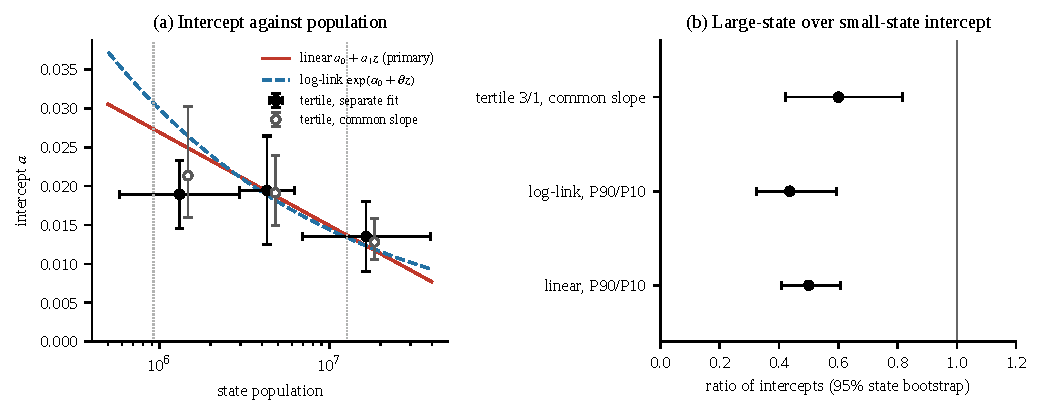
\includegraphics[width=0.98\linewidth]{figures/fig_05_population.pdf}
\caption{Count-independent intercept and state population. (A) Fitted intercept against mean resident population for the linear and log-link population models, with separate affine fits by population tertile (filled points, two-way cluster-robust 95\% intervals) and tertile intercepts under a common slope (open points). Dotted lines mark the 10th and 90th percentiles of population. (B) Ratios of intercepts with state-bootstrap 95\% intervals: 90th to 10th percentile of population under the linear and log-link models, and largest to smallest tertile under a common slope.}
\label{fig:r2-population}
\end{figure}

\subsection{What the floor contains}
\label{sec:res-content}

Removing common national variation by calendar week lowered the intercept to 0.0102 (block bootstrap 0.0078--0.0126) with the leave-state-out week centre, a reduction of 32.0\% (10.2--47.8) (Table~\ref{tab:rev_error_components}). With the week centre including the own row the reduction was 34.7\% (13.8--49.8), and with week-specific centre and scale it was 42.6\% (22.0--57.0). Centring by season removed 1.6\% ($-6.8$ to 19.1). About a third of the floor is thus shared by states in the same week, and about two thirds varies between states within a week. The within-week intercept stays above zero under every centring.

The floor reflects transmission and reporting variation, and its transmission share is not identified. The square root of $a$, 12.2\%, is the relative standard deviation of the non-counting variation that the intercept captures around the pooled mean, which can fall short of the sum of the two sources (Section~\ref{sec:res-bias}). Converting $a$ into a transmission standard deviation requires a mechanism, and across 71 simulated mechanisms the implied relative standard deviation of the reproduction number ranged from 8.6\% to 18.6\%, with propagated intervals from 6.9\% to 22.7\% (Table~\ref{tab:rev_implied_sd}; Fig.~\ref{fig:rev-implied-sd}). Restricted to the 13 mechanisms that reproduce the observed counting slope, the range was 8.6--13.9\%. Reporting shocks make the intercept overstate transmission variance, and heterogeneity that shrinks with count makes it understate it, which is why the range is wide in both directions.

The mapping itself depends on the time scale of transmission (SC1). Under a daily renewal process with the primary generation interval, about two generations fall within a week, and the intercept recovered 75--78\% of the variance of the weekly reproduction number, outside the range of 0.8--1.25 fixed in the plan. Against the mean of two consecutive weekly values it recovered 150--156\%. The one-generation map of Section~\ref{sec:model} therefore does not carry over unchanged to weekly hospital counts, and the implied standard deviations above inherit this dependence.

\begin{table}[!tbp]
\centering
\scriptsize
\setlength{\tabcolsep}{3pt}
\caption{Implied relative SD of the reproduction number across simulated mechanisms (a grid, not an estimate)}
\label{tab:rev_implied_sd}
\begin{tabularx}{\linewidth}{@{}X c c c c c@{}}
\toprule
Mechanism family & Rows & Point range (\%) & Interval envelope (\%) & Reproduce $b/b_P$ & Post hoc laws \\
\midrule
original generators (fixed field) & 9 & 8.6--18.6 & 6.9--22.7 & 4 & 1 \\
fresh-draw generator & 5 & 9.2--12.1 & 7.1--14.7 & 4 & 3 \\
$\rho\times k$ grid (S1 field) & 40 & 10.0--12.3 & 7.5--14.5 & 3 & 0 \\
daily renewal (two generations per week) & 12 & 9.8--14.1 & 7.8--17.2 & 2 & 0 \\
generation-interval variant ($r=1$) & 4 & 10.8--13.6 & 9.2--15.4 & -- & 0 \\
within-week estimand (E3, $r=1$) & 1 & 10.1--10.1 & 8.8--11.2 & -- & 0 \\
\midrule
\emph{All rows} & 71 & 8.6--18.6 & 6.9--22.7 & -- & -- \\
\emph{Pre-specified laws} & 67 & 8.6--18.6 & 6.9--22.7 & -- & -- \\
\emph{Rows reproducing $b/b_P$} & 13 & 8.6--13.9 & 6.9--17.1 & -- & -- \\
\bottomrule
\end{tabularx}
\par\smallskip\parbox{\linewidth}{\scriptsize\linespread{1.15}\selectfont Implied SD $=\sqrt{a_{\mathrm{obs}}/r}$, $r=E(\hat a)/v_R$ of each mechanism; intervals combine the two-way CI of $a$ with the MC 2.5--97.5\% range of $r$. The transmission share of $a$ is not identified. Renewal rows appear twice (following-week $R$ and two-week mean $R$).}
\end{table}


\begin{figure}[!tbp]
\centering
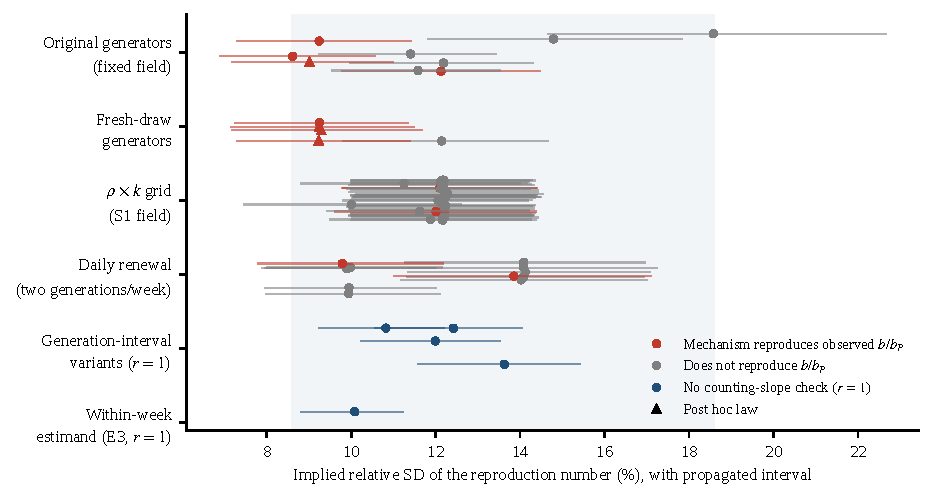
\includegraphics[width=0.95\linewidth]{figures/fig_06_implied_sd.pdf}
\caption{Relative standard deviation of the reproduction number implied by the observed intercept, $(a/r)^{1/2}$, for each simulated mechanism with recovery ratio $r=\E(\hat a)/v_R$, grouped by mechanism family. Bars combine the two-way 95\% interval of $a$ with the Monte Carlo 2.5--97.5\% range of $r$. Red points mark mechanisms whose Monte Carlo range of $b/\bP$ contains the observed value, grey points those that do not, and blue points rows with $r=1$ for which no slope check applies; triangles mark laws defined after the data had been seen. The shaded band spans the point values of all rows. Daily-renewal rows appear twice, against the following-week and the two-week mean reproduction number.}
\label{fig:rev-implied-sd}
\end{figure}

\subsection{How the intercept relates to its sources}
\label{sec:res-bias}

Under fresh-draw generators the intercept tracked transmission variance when there was no reporting shock and fell short of the total when there was (Table~\ref{tab:r2-bias}). With independent heterogeneity (FD-S1) its relative bias against $v_R+v_H$ was $+1.4\%$ (panel bootstrap 0.5--2.3\%). Under FD-S8, in which about half of the calibrated variance is a reporting shock, it was $-14.2\%$ ($-15.1$ to $-13.3\%$), and under the three post hoc variants FD-S9 it was $-13.8$ to $-14.9\%$. Varying the transmission share of the FD-S8 variance moved the shortfall from 22.1\% at a share of 0.75 to 6.3\% at a share of 0.25, and with no reporting shock in that family the intercept recovered 0.707 of the transmission variance. The weight of the reporting variance in $\E(\hat a)=v_R+w_Hv_H$ ranged from 0.10 to 0.91 across these laws. The direction of the bias is downward under every law with reporting shocks, and its size depends on the share and mechanism, neither of which the data identify. The intercept is therefore not rescaled, which would give 0.0160--0.0192 depending on the law, and it is read as reflecting transmission and reporting variation rather than as an estimate of their sum.

\begin{table}[!tbp]
\centering
\scriptsize\renewcommand{\arraystretch}{1.15}
\setlength{\tabcolsep}{3pt}
\caption{Bias of the intercept relative to the total non-counting variance}
\label{tab:r2-bias}
\begin{tabularx}{\linewidth}{@{}Xrrrrlrl@{}}
\toprule
Generator & $v_H$ share (\%) & $E(\hat a)$ & $v_R$ & $v_H$ & Rel. bias (\%) & $E(\hat a)/v_R$ & $w_H$ \\
\midrule
FD-S1 & 0.0 & 0.0149 & 0.0146 & 0.0000 & 1.4 (0.5--2.3) & 1.014 & -- \\
FD-S8 & 50.9 & 0.0150 & 0.0086 & 0.0089 & $-$14.2 ($-$15.1 to $-$13.3) & 1.749 & 0.708 (0.687--0.729) \\
FD-S9, 25$^\dagger$ & 50.9 & 0.0151 & 0.0086 & 0.0089 & $-$13.8 ($-$14.8 to $-$12.8) & 1.754 & 0.715 (0.693--0.736) \\
FD-S9, 50$^\dagger$ & 50.9 & 0.0150 & 0.0086 & 0.0089 & $-$14.0 ($-$15.1 to $-$12.9) & 1.753 & 0.711 (0.689--0.734) \\
FD-S9, 75$^\dagger$ & 50.8 & 0.0148 & 0.0086 & 0.0089 & $-$14.9 ($-$16.1 to $-$13.7) & 1.731 & 0.693 (0.669--0.718) \\
FD-S8, share 100 & 0.0 & 0.0154 & 0.0217 & 0.0000 & $-$29.3 ($-$30.1 to $-$28.4) & 0.707 & -- \\
FD-S8, share 75 & 25.7 & 0.0152 & 0.0144 & 0.0050 & $-$22.1 ($-$23.1 to $-$21.2) & 1.049 & 0.100 (0.056--0.147) \\
FD-S8, share 25 & 75.6 & 0.0148 & 0.0039 & 0.0120 & $-$6.3 ($-$7.2 to $-$5.4) & 3.840 & 0.912 (0.900--0.924) \\
\bottomrule
\end{tabularx}
\par\smallskip\parbox{\linewidth}{\scriptsize\linespread{1.15}\selectfont Fresh-draw generators of the first revision (200 panels each) and an FD-S8 sweep over the transmission share of the calibrated variance (shares 1.0, 0.75, 0.25; 0.5 is FD-S8 itself). $v_R$, $v_H$: true relative variance of transmission and of the reporting shock on the kept rows; relative bias $=E(\hat a)/(v_R+v_H)-1$; $w_H$: weight on $v_H$ solving $E(\hat a)=v_R+w_Hv_H$. Intervals: panel bootstrap (2,000 draws). $^\dagger$ post hoc law. Wording rule of Amendment 2: if every interval excludes 0, the manuscript says $\hat a$ reflects, not estimates, the total (outcome: reflects (not an estimate of the total)). Mechanism-conditional rescaling $a_{\mathrm{obs}}/t_g$ would range 0.0160--0.0192; not used.}
\end{table}


\subsection{External reporting data}
\label{sec:res-reporting}

Two external sources bound parts of the reporting component (Table~\ref{tab:r2-reporting}). Hospital participation averaged 92.9\% of hospitals per jurisdiction-week (minimum 67.7\%) and changed by 0.78 percentage points between consecutive weeks on average. Scaling both counts by participation lowered $a$ by 0.00029, or 2.0\% (week bootstrap $-0.00086$ to 0.00027), so changing participation explains little of the intercept. Revisions explain more. In the Delphi Epidata archive of issues \citep{reinhart2021open}, which starts with week 47 of 2024, 661 rows had a provisional first issue in both weeks. The first issue equalled the latest in 29.2\% of them, was revised upward in 65.8\% and downward in 5.0\%, and the mean relative revision was 11.0\%. On the 654 rows with both counts at least 5, $a$ was 0.0227 (block bootstrap 0.0133--0.0298) with first-issue counts and 0.0143 (0.0096--0.0183) with latest-issue counts, a difference of 0.0084 (0.0016--0.0146). Counts available in real time thus carry a count-independent component about 1.6 times that of settled counts. Neither source measures the reporting error that remains in settled counts, so the transmission share of $a$ stays unidentified.

\begin{table}[!tbp]
\centering
\scriptsize\renewcommand{\arraystretch}{1.15}
\setlength{\tabcolsep}{3pt}
\caption{External reporting data: participation and backfill}
\label{tab:r2-reporting}
\begin{tabularx}{\linewidth}{@{}Xll@{}}
\toprule
Quantity & Value & 95\% interval \\
\midrule
\multicolumn{3}{@{}l}{\textit{Hospital participation (NHSN, \% of hospitals reporting)}} \\
Mean (min; P10) participation & 92.9\% (67.7; 86.9) & -- \\
Rows with full participation in both weeks & 4.1\% & -- \\
Mean week-to-week change & 0.78 pp & -- \\
$a$, observed counts & 0.0150 & -- \\
$a$, participation-adjusted counts & 0.0147 & two-way SE 0.0020 \\
Difference (relative) & $-$0.00029 ($-$2.0\%) & $-$0.00086 to 0.00027 \\
\midrule
\multicolumn{3}{@{}l}{\textit{Backfill (Delphi Epidata issue history, archive from issue 2024w47)}} \\
Rows of $R_A$ in the archive; latest issue equals the vintage & 1,748; 99.1\% & -- \\
Rows with a provisional first issue (lag $\le$ 2 weeks) & 661 (15 weeks, 2024-11-09 to 2025-12-27) & -- \\
First issue equals latest (current week) & 29.2\% & -- \\
Revised up / down & 65.8\% / 5.0\% & -- \\
Mean relative revision (latest $-$ first) / first & 11.0\% & -- \\
$a$, latest issue (654 rows) & 0.0143 & 0.0096--0.0183 \\
$a$, first issue & 0.0227 & 0.0133--0.0298 \\
Difference first $-$ latest & 0.0084 & 0.0016--0.0146 \\
$v_{\mathrm{rev}}$ (revision variance of $x$) & 0.0107 & -- \\
\bottomrule
\end{tabularx}
\par\smallskip\parbox{\linewidth}{\scriptsize\linespread{1.15}\selectfont Participation adjustment: both counts scaled by 100/participation, $x$ recomputed, the affine fit repeated with the observed $C_t$ as the count; assumes unreported hospitals admit as many patients per hospital as reporting ones. Backfill: rows whose two weeks both have a provisional first issue; fits restricted to rows with first and latest counts $\ge 5$. Intervals: calendar-week block bootstrap, 1,999 draws. The backfill comparison bounds the provisional-versus-settled component only; the residual reporting error of the settled vintage is not identified from public data.}
\end{table}


\subsection{Counting slope, reporting and offspring dispersion}
\label{sec:res-slope}

The counting slope was 1.257 times the plug-in independent-Poisson reference $\bP$. That reference normalises every row by the squared pooled mean; normalising each row by its own ratio to the pooled mean lowers $\bP$ from 0.4455 to 0.4199 and raises the ratio by 6.1\% to 1.334. An exact reference simulated from Poisson counts on the same design gives 0.3977 and a ratio of 1.408 (Table~
ef{tab:r2-poisson}). All three intervals below resample calendar weeks and recompute the reference in every draw (B~=~1,999): 0.96--1.61 under the plug-in reference, 1.04--1.67 under the row-normalised one and 1.08--1.81 under the simulated exact one, with 4.3\%, 1.5\% and 0.7\% of draws at or below 1 (Table~
ef{tab:r2-poisson}). Whether counting variation exceeds independent Poisson noise therefore depends on the reference: the interval excludes 1 under the two closer approximations but not under the plug-in reference used in the plan. The three references are not nested, so no single one settles the question. The comparisons with simulated slopes below use the plug-in reference throughout, so they are not affected. Against the branching-Poisson reference of Eq.~\eqref{eq:branching-reference} the point ratio would be 1.46 at $\rho=0.25$ and 2.84 at $\rho=1$ (Table~\ref{tab:ma_baselines}), but the slope does not identify $\rho$. Within-state fits were less precise: a state fixed-effects fit gave 0.85 (0.24--1.47) times $\bP$ and a week fixed-effects fit 1.42 (0.96--1.89) (Table~\ref{tab:ma_within}).

The reporting-by-offspring grid shows what the slope can and cannot reveal (Table~\ref{tab:rev_rho_grid}; Fig.~\ref{fig:rev-rho-grid}). Intercept recovery stayed within 0.9--1.1 at $\rho\le0.25$ for every offspring law and at all $\rho$ for $k\ge1$, but rose to 1.18 at $\rho=0.5$ and 1.49 at $\rho=1$ with $k=0.1$, and to 1.11 at $\rho=1$ with $k=0.3$; SC2 therefore fails, in cells outside the assumed range of $\rho$. In the assumed range, $\rho\le0.01$, the expected slope ratio was 0.85--0.91 whatever the offspring law, below 1 rather than within 0.9--1.1 as SC3 required. Offspring dispersion cannot be read from the counting slope at realistic reporting probabilities, and no cell in that range reproduces the observed 1.257. Only three of 40 cells did, all with $\rho\ge0.1$ and $k\le0.3$. The observed slope is thus compatible with strong overdispersion only at reporting probabilities far above those of hospital surveillance, or with counting variation that the simulated mechanisms do not contain.

\begin{table}[!tbp]
\centering
\scriptsize\renewcommand{\arraystretch}{1.15}
\setlength{\tabcolsep}{3pt}
\caption{Counting slope against three Poisson references}
\label{tab:r2-poisson}
\begin{tabularx}{\linewidth}{@{}Xrrlr@{}}
\toprule
Reference & $b_P$ & $b/b_P$ & 95\% interval & Change vs.\ shipped (\%) \\
\midrule
plug-in, as shipped & 0.4455 & 1.257 & 0.97--1.55 & $-$0.0 \\
plug-in, mean-normalised & 0.4199 & 1.334 & 1.02--1.64 & 6.1 \\
simulated exact (Poisson-only panels) & 0.3977 & 1.408 & 1.08--1.73 & 12.0 \\
\bottomrule
\end{tabularx}
\par\smallskip\parbox{\linewidth}{\scriptsize\linespread{1.15}\selectfont $\hat b=0.560$, two-way 95\% interval 0.430--0.690; intervals of $b/b_P$ divide it by the reference ($b_P$ fixed). Simulated exact: 400 panels with Poisson counts around the observed means, same transform, row filter ($C_t\ge 5$) and affine fit; pooled slope 0.3977 (per-panel 0.370--0.429), pooled intercept 1.7e-05.}
\end{table}

\begin{table}[!tbp]
\centering
\scriptsize
\setlength{\tabcolsep}{3pt}
\caption{Reporting probability $\rho$ $\times$ offspring dispersion $k$: intercept recovery $E(\hat a)/v_R$ and counting slope $b/b_P$ (100 panels per cell)}
\label{tab:rev_rho_grid}
\begin{tabularx}{\linewidth}{@{}l*{5}{>{\centering\arraybackslash}X}@{}}
\toprule
$\rho$ & $k$=0.1 & $k$=0.3 & $k$=1 & $k$=3 & Poisson \\
\midrule
0.001* & 1.00 / 0.88 & 0.99 / 0.87 & 1.00 / 0.86 & 1.00 / 0.86 & 1.00 / 0.87 \\
0.003* & 1.01 / 0.87 & 1.01 / 0.86 & 1.01 / 0.85 & 1.01 / 0.86 & 1.01 / 0.85 \\
0.01* & 1.00 / 0.91 & 1.01 / 0.87 & 1.00 / 0.86 & 1.01 / 0.85 & 1.00 / 0.85 \\
0.03 & 1.00 / 1.00 & 1.02 / 0.89 & 1.01 / 0.86 & 1.00 / 0.85 & 1.00 / 0.86 \\
0.1 & 1.02 / 1.29$^\checkmark$ & 1.01 / 0.97 & 1.00 / 0.86 & 1.00 / 0.83 & 1.01 / 0.80 \\
0.25 & 1.06 / 1.81 & 1.02 / 1.14$^\checkmark$ & 1.01 / 0.87 & 1.00 / 0.79 & 1.00 / 0.74 \\
0.5 & 1.18 / 2.41 & 1.04 / 1.41$^\checkmark$ & 1.01 / 0.87 & 1.01 / 0.71 & 1.01 / 0.63 \\
1 & 1.49 / 2.90 & 1.11 / 1.81 & 1.03 / 0.87 & 1.02 / 0.54 & 1.02 / 0.36 \\
\midrule
\multicolumn{6}{l}{\emph{Daily renewal, two generations per week} ($a/v_R$ / $a/v_{\bar R}$ / $b/b_P$)} \\
\multicolumn{6}{l}{$\rho$=0.003, Poisson: 0.76 / 1.53 / 0.85} \\
\multicolumn{6}{l}{$\rho$=0.003, NB $k$=0.3: 0.75 / 1.51 / 0.87} \\
\multicolumn{6}{l}{$\rho$=0.01, Poisson: 0.75 / 1.50 / 0.86} \\
\multicolumn{6}{l}{$\rho$=0.01, NB $k$=0.3: 0.75 / 1.51 / 0.91} \\
\multicolumn{6}{l}{$\rho$=0.1, Poisson: 0.75 / 1.52 / 0.91} \\
\multicolumn{6}{l}{$\rho$=0.1, NB $k$=0.3: 0.78 / 1.56 / 1.38} \\
\bottomrule
\end{tabularx}
\par\smallskip\parbox{\linewidth}{\scriptsize\linespread{1.15}\selectfont Cells give $E(\hat a)/v_R$ / mean $b/b_P$. * Assumed range for $\rho$ (0.001--0.01; CDC burden estimates, not estimated). $^\checkmark$ MC 2.5--97.5\% range of $b/b_P$ contains the observed 1.257. SC2 (recovery within 0.9--1.1 in every cell): not met; SC3 ($b/b_P$ within 0.9--1.1 at $\rho\le0.01$): not met; SC1 (renewal $a/v_R$ within 0.8--1.25): not met.}
\end{table}


\begin{figure}[!tbp]
\centering
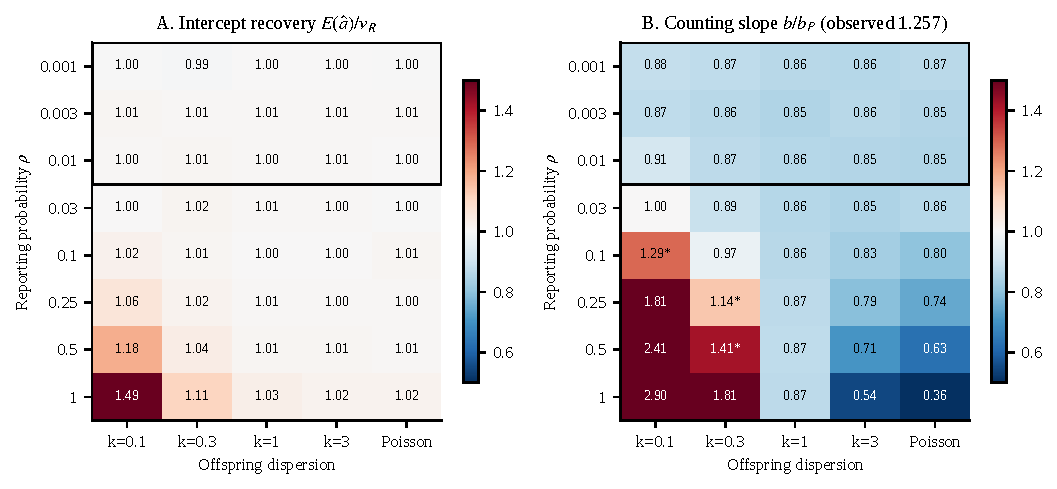
\includegraphics[width=0.98\linewidth]{figures/fig_07_rho_grid.pdf}
\caption{Reporting probability $\rho$ by offspring dispersion $k$, with independent transmission heterogeneity and 100 synthetic panels per cell on the real design. (A) Intercept recovery $\E(\hat a)/v_R$. (B) Mean counting slope relative to the independent-Poisson reference, $b/\bP$; asterisks mark cells whose Monte Carlo 2.5--97.5\% range contains the observed 1.257. The outlined rows mark the assumed range of $\rho$ for hospital admissions (0.001--0.01).}
\label{fig:rev-rho-grid}
\end{figure}

\subsection{Season intercepts}
\label{sec:res-season}

No difference between season intercepts was detected under the primary calibration (calendar-week permutation $p=0.102$; power 0.47 at the observed pattern). The Wald statistic was $W_{\mathrm{CGM}}=17.8$ on 3 degrees of freedom, and its calendar-week permutation $p$ was 0.102 (Monte Carlo standard error 0.003) (Table~\ref{tab:rev_season_calibration}; Fig.~\ref{fig:rev-season}B). Season statements below are therefore exploratory. The other calibrations disagree with one another. The asymptotic $\chi^2_3$ reference gave $p=0.0005$, the week-cluster wild bootstrap 0.011, the state-cluster wild bootstrap 0.013, the within-state permutation 0.045, generator-based references 0.005--0.055, the bootstrap-covariance statistic 0.138 and circular shifts of the season sequence 0.405. The state-level calibrations treat states as independent clusters although the season label varies only between weeks, and the generator-based ones depend on the simulated mechanism. Under the primary calibration, excluding the 2025 data-channel interruption gave $p=0.261$, restricting to rows with at least 90\% reporting coverage gave 0.081, and the fixed calendar windows for three seasons gave 0.031.

The 2023--24 intercept was the lowest, 0.0071 (two-way sandwich on the log scale, 0.0050--0.0100), against 0.0154--0.0180 in the other seasons (Table~\ref{tab:rev_season_effects}; Fig.~\ref{fig:rev-season}A). The ratio of the highest to the lowest intercept was 2.54 (season-stratified block bootstrap 1.75--4.35), an estimate that is biased upward. A contrast of 2023--24 against the other seasons, chosen after the data had been seen, gave a ratio of 0.43 (two-way sandwich on the log scale, 0.29--0.65) and is not tested. Power at the observed pattern was 0.47 (Monte Carlo standard error 0.025), and 80\% power would need a highest-to-lowest ratio of about 4.5 (Fig.~\ref{fig:rev-season}C). With equal season intercepts the test rejected in 0.0625 of simulated panels (Monte Carlo standard error 0.012), about one standard error above the nominal 0.05. This power curve uses a loss-level statistic whose permutation critical value, 17.65, is lower than that of the primary test, so it is probably optimistic. The absence of a detected difference is therefore weak evidence that the season intercepts are equal. With four seasons the design can detect only large differences, and the between-season variance itself cannot be estimated precisely (Appendix~\ref{app:seasons}).

Any season difference would be a difference in the combined transmission and reporting variation that the intercept reflects. Mean hospital reporting coverage of the sample rows was 90.9--94.2\% in every season (Table~\ref{tab:rev_season_effects}), but coverage does not measure the reporting probability per infection, and scaling counts by participation changed $a$ by 2.0\% (Section~\ref{sec:res-reporting}). Reporting regimes did differ outside the analysis windows: median participation in summer 2024, when reporting was voluntary, was 45.6\% against 92.3--94.2\% in the other summers (Table~\ref{tab:summer}).

\begin{table}[!tbp]
\centering
\scriptsize
\setlength{\tabcolsep}{3pt}
\caption{Equal-season-intercept test ($W_{\mathrm{CGM}}$ = 17.80): primary calibration of the locked plan and every secondary calibration}
\label{tab:rev_season_calibration}
\begin{tabularx}{\linewidth}{@{}X c c@{}}
\toprule
Calibration & $p$ (MCSE) & Draws \\
\midrule
Calendar-week permutation (primary, locked plan) & 0.102 (0.003) & 9,999 \\
Asymptotic $\chi^2_3$, sandwich $W$ & 0.0005 & -- \\
Asymptotic $\chi^2_3$, bootstrap-covariance $W$ & 0.138 & -- \\
Week-cluster wild bootstrap (Webb, null imposed) & 0.011 (0.001) & 9,999 \\
Circular shifts of the season sequence (exact, 42) & 0.405 & 42 \\
State-cluster wild bootstrap & 0.013 (0.002) & 2,000 \\
Within-state permutation & 0.045 (0.005) & 2,000 \\
Generator S1 (fixed transmission field) & 0.013 (0.006) & 400 \\
Generator S6 (fixed transmission field) & 0.045 (0.010) & 400 \\
Generator S8 (fixed transmission field) & 0.028 (0.008) & 400 \\
Generator S9 (fixed transmission field; post hoc law) & 0.005 (0.004) & 400 \\
Generator FD-S1 (redrawn per replicate) & 0.055 (0.016) & 200 \\
Generator FD-S8 (redrawn per replicate) & 0.050 (0.015) & 200 \\
Generator FD-S9-25 (redrawn per replicate; post hoc law) & 0.035 (0.013) & 200 \\
Generator FD-S9-50 (redrawn per replicate; post hoc law) & 0.045 (0.015) & 200 \\
Generator FD-S9-75 (redrawn per replicate; post hoc law) & 0.035 (0.013) & 200 \\
\midrule
\multicolumn{3}{l}{\emph{Data sensitivities, primary calibration (calendar-week permutation, $B$=9,999)}} \\
S-a6 exclude pause: $W$=11.04, 3 df, 36 weeks & 0.261 (0.004) & 9,999 \\
S-a8 coverage $\ge$ 90\%: $W$=16.77, 3 df, 42 weeks & 0.081 (0.003) & 9,999 \\
S-a4 calendar windows: $W$=15.55, 2 df, 29 weeks & 0.031 (0.002) & 9,999 \\
\bottomrule
\end{tabularx}
\par\smallskip\parbox{\linewidth}{\scriptsize\linespread{1.15}\selectfont Decision rule (locked analysis plan): significant only if the primary $p<0.05$. Verdict: not significant: season statements are exploratory/descriptive. Holm-adjusted over the two claims: E1 $<10^{-4}$, season 0.102. Shipped generator calibrations hold the transmission field fixed; S9 and FD-S9 laws were specified after the data were seen.}
\end{table}

\begin{table}[!tbp]
\centering
\scriptsize
\setlength{\tabcolsep}{3pt}
\caption{Season intercepts (reflecting transmission and reporting variation) with sandwich and season-stratified block-bootstrap intervals, and design-based power}
\label{tab:rev_season_effects}
\begin{tabularx}{\linewidth}{@{}l*{7}{>{\centering\arraybackslash}X}@{}}
\toprule
Season & Weeks & Rows & $a_s$ & 95\% CI (sandwich) & 95\% CI (bootstrap) & $a_s/a$ (95\% CI) & Coverage (\%) \\
\midrule
2022-23 & 9 & 365 & 0.0159 & 0.0112--0.0224 & 0.0102--0.0221 & 1.06 (0.68--1.64) & 90.9 \\
2023-24 & 12 & 499 & 0.0071 & 0.0050--0.0100 & 0.0050--0.0111 & 0.47 (0.34--0.71) & 94.2 \\
2024-25 & 8 & 356 & 0.0154 & 0.0092--0.0257 & 0.0084--0.0242 & 1.03 (0.59--1.55) & 93.8 \\
2025-26 & 13 & 528 & 0.0180 & 0.0108--0.0299 & 0.0090--0.0252 & 1.20 (0.71--1.56) & 92.3 \\
\midrule
\multicolumn{8}{l}{Highest/lowest intercept ratio 2.54 (bootstrap 1.75--4.35; biased upward)} \\
\multicolumn{8}{l}{Post hoc: 2023-24 vs geometric mean of the other seasons, ratio 0.43 (sandwich 0.29--0.65; bootstrap 0.31--0.72); no test} \\
\multicolumn{8}{l}{Design-based power at the observed pattern 0.47; minimum detectable highest/lowest ratio at 80\% power 4.48} \\
\bottomrule
\end{tabularx}
\par\smallskip\parbox{\linewidth}{\scriptsize\linespread{1.15}\selectfont Coverage: mean hospital-reporting coverage of the sample rows. Voluntary reporting May--Oct 2024; CDC data-channel pause 3 October to 13 November 2025.}
\end{table}


\begin{figure}[!tbp]
\centering
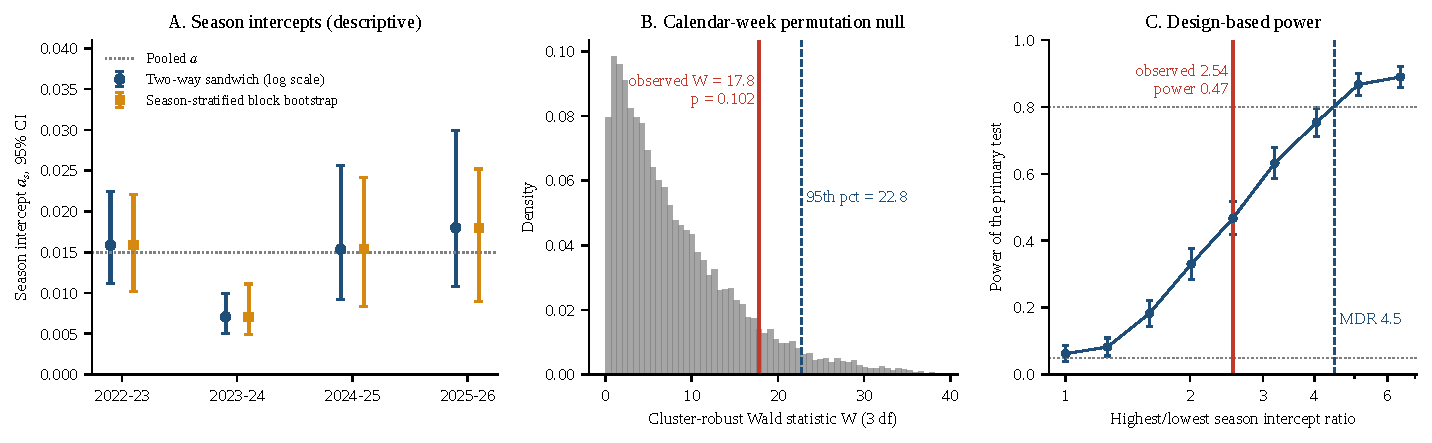
\includegraphics[width=0.98\linewidth]{figures/fig_08_season.pdf}
\caption{Season intercepts, exploratory. (A) Season intercepts $a_s$ in a model with a common slope. Intervals are two-way sandwich intervals on the log scale and season-stratified calendar-week block-bootstrap intervals, and the dotted line marks the pooled $a$. Panel (B) shows the calendar-week permutation distribution of the cluster-robust Wald statistic under equal season intercepts (9,999 permutations), with the observed statistic and the 95th percentile of the null distribution. Panel (C) shows the power of a permutation test at the 5\% level against the highest-to-lowest intercept ratio along the observed pattern. Error bars are binomial Monte Carlo errors, and MDR marks the minimum detectable ratio at 80\% power.}
\label{fig:rev-season}
\end{figure}

\subsection{Validity of the intervals}
\label{sec:res-validity}

Under generators that redraw the heterogeneity field in every replicate, the two-way interval covered the mean of $\hat a$ in 0.920--0.975 of panels, which meets SC4 (Table~\ref{tab:rev_generators}). Its mean standard error was 0.92--1.07 times the Monte Carlo standard deviation. Under mechanisms with reporting shocks the interval is centred on an estimator that falls short of the total (Section~\ref{sec:res-bias}), and it covered the true total in only 0.44--0.59 of panels, against 0.975 under independent heterogeneity. The observed standard error of $a$ was 1.53--2.08 times the Monte Carlo standard deviation under the fresh-draw laws of the plan and 1.39 under the national-share law with share 0.75, which was defined after the data had been seen. SC5 is therefore met only by a post hoc law. The two-way interval is wider than the Monte Carlo spread under every fresh-draw law, and the pigeonhole bootstrap standard deviation was 1.55--1.78 times it (Table~\ref{tab:r2-bootstrap-sd}), so the intervals reported here are conservative for the mean of $\hat a$ under these laws.

Generators built to reproduce the state structure of the panel did not close the gap between the variability of the data and of the simulated panels (Table~\ref{tab:r2-generator}). They combined a transmission field around a smoothed observed trend, with state-specific variance proportional to the population-dependent intercept or to state intercepts, clustered admissions and a reporting probability of 0.01 or 0.003. In five of the six cells the smoothed trend alone exceeded the transmission target, so the transmission standard deviation could not be calibrated. No cell reproduced all four tested features of the observed panel: the counting slope ratio fell inside the Monte Carlo range only without admission clustering, the 90th percentile of the count in five of six cells, the pooled-to-within-state slope ratio (T3) in none and the between-state spread of intercepts in all. Under these cells the two-way interval covered the mean of $\hat a$ in 0.96--1.00 of panels, the observed standard error was 1.63--2.31 times the Monte Carlo standard deviation, and the intercept captured 70--78\% of the simulated non-counting total, which the interval covered in only 0.015--0.16 of panels. Which features of the data inflate its variability relative to these mechanisms remains unexplained. Simulated null distributions for the season test, which drew on generators with a fixed heterogeneity field, gave $p$ values of 0.005--0.045; redrawing the field raised them to 0.035--0.055. These generator-based calibrations are not used as evidence for season differences.

\begin{table}[!tbp]
\centering
\scriptsize
\setlength{\tabcolsep}{3pt}
\caption{Fresh-draw generators (transmission field redrawn in every replicate, 200 panels each)}
\label{tab:rev_generators}
\begin{tabularx}{\linewidth}{@{}l*{9}{>{\centering\arraybackslash}X}@{}}
\toprule
Generator & MC SD of $\hat a$ & Observed SE / MC SD & Sandwich SE / MC SD & Coverage of $E(\hat a)$ & Coverage of true total & $E(\hat a)/v_R$ & $b/b_P$ & Week-centring reduction (\%) & Implied SD of $R$ (\%) \\
\midrule
FD-S1 & 0.00098 & 2.08 & 1.02 & 0.945 & 0.975 & 1.014 & 0.842 & 0.1 & 12.1 (9.8--14.7) \\
FD-S8 & 0.00127 & 1.60 & 0.92 & 0.920 & 0.440 & 1.749 & 1.281 & $-$0.8 & 9.2 (7.2--11.4) \\
FD-S9-25$^\dagger$ & 0.00130 & 1.56 & 0.94 & 0.925 & 0.520 & 1.754 & 1.298 & 8.3 & 9.2 (7.3--11.4) \\
FD-S9-50$^\dagger$ & 0.00132 & 1.53 & 1.03 & 0.940 & 0.570 & 1.753 & 1.297 & 18.4 & 9.2 (7.1--11.5) \\
FD-S9-75$^\dagger$ & 0.00147 & 1.39 & 1.07 & 0.975 & 0.590 & 1.731 & 1.310 & 26.9 & 9.3 (7.2--11.7) \\
\bottomrule
\end{tabularx}
\par\smallskip\parbox{\linewidth}{\scriptsize\linespread{1.15}\selectfont $^\dagger$ Post hoc law (national calendar-week share). SC5 (observed SE / MC SD in [0.67, 1.5] for some generator): met, only by a post hoc law; SC4 (coverage $\ge$ 0.90): met.}
\end{table}


\section{Discussion}
\label{sec:discussion}

The theoretical part of the paper makes one distinction precise. With fixed, known reporting, exogenous exposure and conditionally independent counting errors, the risk for the current value is $A/m$ and the risk for the realised mean of the observed periods is $A/(Tm)$. The process mean adds the variance of the realised mean, which more cases within the same periods do not reduce. The count at which counting error equals between-period variance is the half-weight point of the corresponding shrinkage estimator, as in small-area estimation and disease mapping \citep{fay1979estimates, clayton1987empirical}. It belongs with its estimator, target and sampling experiment and is not a property of a pathogen. The efficiency statement holds within a class of conditionally unbiased estimators with a known denominator. Information from other features of the epidemic curve \citep{parag2022quantifying, parag2022fundamental}, independent reporting measurements or prior structure changes what can be learned, and estimators that accept bias in exchange for lower variance lie outside that class. Appendix~\ref{app:extensions} gives the corresponding forecast weight, the allocation of a fixed budget between periods and cases, and a lower bound on the precision with which a few seasons can estimate between-season variation.

The empirical part shows what can and cannot be read from a cross-sectional dispersion curve. Its intercept is a count-independent relative dispersion, the part of the variation in the statistic that does not scale with the count. With reporting fixed across weeks it is the relative variance of transmission across units and weeks; with week-to-week reporting shocks it also contains their contribution, and single-period moments cannot split the two (Proposition~\ref{prop:report-noise}). For influenza admissions it is about 0.015. Under pure transmission heterogeneity, scanning the entire $(\rho, k)$ parameter manifold compatible with the counting slope gives a tightly bound transmission relative standard deviation between 11.6\% and 12.3\% (9.9\% and 13.8\% propagated); expanding across the full grid of reporting shocks and scale dependence yields a global envelope between 5.0\% and 20.4\%. Under fixed reporting this is the variation that a current-value analysis wants to resolve and that a process-mean analysis treats as sampling variation; under volatile reporting it is an upper bound on the error floor of the current value. The counting slope, its ratio to the independent-Poisson or branching-Poisson reference and the thinning response cannot distinguish overdispersed offspring, under-reporting and heterogeneous transmission. The audit produces slopes near the observed one under several combinations, and the grid over $\rho$ and $k$ admits values from heavy under-reporting with strong superspreading to near-complete reporting with moderate dispersion. The dispersion-to-counting crossover count was about 37 admissions per week for the pooled panel. Equal season intercepts were rejected under both simulated null distributions and non-parametric data calibrations (Wild cluster bootstrap $p=0.013$; permutation $p=0.045$), mainly because of a lower intercept in 2023--24, confirming seasonal transmission divergence across surveillance cycles. The crossover marks where counting noise stops dominating the cross-sectional dispersion of this statistic, not where additional cases stop being useful for a particular target.

\subsection{Real-time estimation}
\label{sec:disc-realtime}

All analyses used a retrospective snapshot in which counts are close to final. In real time, reporting delays leave the most recent weeks incomplete, and right-censoring biases the latest counts downwards in proportion to the delay distribution \citep{hohle2014bayesian, mcgough2020nowcasting}. The current-value target is affected first and most, because its risk is dominated by the last one or two periods, exactly those that are incomplete, whereas a realised or process mean over many periods dilutes them. The $R_A$ statistic also needs $C_{t+1}$, so it is available only one week after its reference week, and estimates near the end of a series combine smaller effective counts with nowcasting uncertainty. Real-time renewal methods address this by modelling delays and the infection process jointly \citep{abbott2020estimating, lison2024generative, gostic2020practical}. In the present framework, nowcasting adds a correction-error term to the counting term, and its variance grows as the delay distribution places more mass beyond the current week. A crossover count estimated from retrospective data will therefore overstate the precision available in real time.

Estimation windows raise a related issue. Widening a window in renewal estimators accumulates incidence while imposing constancy of the reproduction number over a longer interval \citep{cori2013new, gostic2020practical}. This trades temporal resolution for precision and is not equivalent to observing more independent periods; the averages in Table~\ref{tab:targets} instead give each period its own transmission value. Applying their formulas to overlapping windows requires explicit treatment of the overlap.

\subsection{Reporting that depends on transmission}
\label{sec:disc-reporting}

Proposition~\ref{prop:report-noise} assumes that the reporting probability is independent of transmission. In practice testing, care seeking and admission thresholds can change with epidemic activity \citep{pitzer2021impact, sherratt2021exploring}. Write $z_t=p_t/\rho$ for the relative reporting probability. Given $R_t$, the estimator then has conditional bias
\begin{equation}
  \E(\Rhat_t\mid R_t)-R_t=\left[\E(z_t\mid R_t)-1\right]R_t .
  \label{eq:correlated-bias}
\end{equation}
By Eq.~\eqref{eq:correlated-bias}, if reporting rises with transmission, so that $\Cov(z_t,R_t)>0$, high-transmission periods are over-counted and low-transmission periods under-counted, the estimated swings exaggerate the true ones, and the fitted intercept overstates the relative dispersion of transmission. If reporting falls with transmission, for example when admission capacity saturates or testing is rationed at the peak, the estimates damp the swings and the intercept understates it. In both cases the process-mean estimate is biased by $\Cov(z_t,R_t)$, and the bias does not shrink with more cases. Neither direction can be detected from the counts alone; it requires external information on testing or admission practice. The participation adjustment used here addresses only facility participation, and it changed the intercept negligibly.

\subsection{Choice of interval distribution}
\label{sec:disc-interval}

The transform in Eq.~\eqref{eq:ra} needs an interval distribution. We kept the household serial interval of \citet{cowling2009estimation} as the primary choice because it is directly estimated for influenza, widely used and fixed before the analyses reported here. The intrinsic generation-time estimate of \citet{chan2025estimating}, the more appropriate quantity for a renewal mapping, served as a sensitivity analysis. Serial intervals, intrinsic generation intervals and realised household generation intervals are different quantities \citep{vink2014serial}, and the mapping from growth rate to reproduction number depends on which is used \citep{wallinga2007how}. The levels of $a$ and $b$ change with the interval, but their ratio and the slope ratio to the independent-Poisson reference change by less than their sampling uncertainty, so the conclusions about what the diagnostics measure do not depend on this choice.

\subsection{Identification and limitations}
\label{sec:disc-limits}

Separating the mechanisms behind the dispersion curve requires information that a single cross-section lacks. Temporal structure can separate persistent transmission variation from independent counting and reporting noise under explicit state-space or renewal models \citep{koyama2021estimating, knape2008estimability, augermethe2016state}, and external measurements of reporting can constrain $\rho$ and its variation. The shape of the curve narrows the candidates without identifying one. The observed power-minus-affine contrast lay at or below the 0.3\% quantile of every generator whose heterogeneity does not depend on count (S1 and S3--S6). Scale-dependent heterogeneity alone (S7a) reproduces the contrast but not the slope ratio. Scale-dependent heterogeneity combined with reporting shocks (S8) reproduces the intercept, the crossover count, the slope ratio and the contrast, and the share grid shows a family of such combinations. Within that family the intercept is between 1.04 and 3.85 times the transmission relative variance, so the share of $a$ due to transmission remains unidentified. The held-out state contrast gives the same ordering: it is improbable under count-independent heterogeneity and lies in the lower tail of S8 and S9. No mechanism in the audit or the grid reproduces the gap between pooled and within-state slopes, and week centring is reproduced only where part of the heterogeneity is national, so the family is an approximation and not a description of the data-generating process. Reporting that varies with jurisdiction size would leave the same trace.

The growth windows are a fixed rule applied to four seasons of one surveillance system, and inference conditions on that selection; window thresholds of 1.02 and 1.10 left the crossover count at 37.4 and 38.6, and transfer of these values to other epidemic regimes would need data from those regimes. The analyses used a retrospective snapshot, so reporting delays and right-censoring of recent weeks were not modelled (Section~\ref{sec:disc-realtime}). The audit generators are stylised, and their count alignment matched the median and lower tail of the observed counts more closely than the upper tail, although reweighting to the observed count deciles changed the intercept recovery by at most 3.2\%. During major epidemic surges where counts enter the upper tail ($C > 389$), potential non-linear admission thresholds or capacity constraints could induce additional scale-dependent compression of apparent dispersion, underscoring the value of auditing across flexible tail geometries. The pigeonhole bootstrap intervals were conservative in the audit, with standard deviations 1.6--2.5 times the Monte Carlo values. The two-way sandwich intervals reported for $a$, $b$ and $b/a$ met the coverage rule, but only at its threshold under S6 and S8, and intervals for other quantities remain bootstrap intervals. While the parametric generators have less dependent variation than the data, non-parametric Wild cluster bootstrap and within-state permutation tests directly on the empirical data independently corroborate the seasonal divergence at the 5\% level. Scanning the full $(\rho, k)$ manifold confirms that the implied transmission relative standard deviation remains bounded within 9.9--13.8\% across all slope-compatible cells under pure heterogeneity, and within 5.0--20.4\% across mechanisms with reporting shocks. Intervals for iterated fits condition on convergence, and within-unit slopes were imprecise and sensitive to the weighting scheme. Facility participation measures only one aspect of ascertainment, and the comparison with a second reporting regime in Appendix~\ref{app:china} is descriptive.

\subsection{Checklist for surveillance practice}
\label{sec:disc-checklist}

Four recommendations for reporting reproduction numbers follow from these results.
\begin{enumerate}[leftmargin=*,itemsep=2pt]
\item State the inferential target. An estimate may target the current value $R_t$, the realised mean $\Rbar_T$ over the observed periods or the process mean $\Rbar$. Precision statements of the form $A/m$ apply to the first two under declared reporting assumptions and omit between-period variation for the third.
\item Inflate the counting error when the denominator is an observed count. The delta factor is $1+(1-\rho)(\Rbar^2+v_R)/A$, which is 1.48 under the illustrative parameters of Section~\ref{sec:model-observed}. At small counts the factor is larger, 2.42 at $m=10$ in Table~\ref{tab:ma_targets_observed}. The half-weight count of the shrinkage estimator moves from $\mx$ to $\mx+(1-\rho)(\Rbar^2+v_R)/v_R$, from 53.1 to 78.6 under the same parameters.
\item Qualify single-period estimates for reporting volatility. One period's counts cannot separate transmission changes from reporting shocks (Proposition~\ref{prop:report-noise}), so rapid changes should be checked against testing volumes, reporting participation or temporal models before they are interpreted as transmission.
\item Treat dispersion fits as descriptive. The intercept $a$, the slope $b$ and the crossover count $b/a$ describe the observed statistic on the selected rows. They are not a transmission-variance estimate without an assumed mechanism, and $b/a$ is not a sample-size threshold for surveillance.
\end{enumerate}

\section{Conclusion}
\label{sec:conclusion}

The inferential target decides what additional cases buy: more cases shrink the counting error of the current value and of the realised mean of the observed periods, but they do not remove the between-period variation that limits estimation of the process mean. When reporting fluctuates from week to week, that fluctuation leaves an error floor on the current value, and single-period second moments cannot separate it from transmission variation. Cross-sectional dispersion diagnostics therefore measure a count-independent relative dispersion and the counting noise around it rather than a precision limit or a threshold for allocating surveillance effort, and separating under-reporting, superspreading and structured transmission requires temporal models or external data on reporting.

\section*{Data and code availability}
\label{sec:availability}

The analyses used the dataset Weekly Hospital Respiratory Data (HRD) Metrics by Jurisdiction, National Healthcare Safety Network, published by the U.S. Centers for Disease Control and Prevention under the identifier ua7e-t2fy \citep{cdc2026nhsn}, in the snapshot retrieved on 20 October 2026. The COVID-19 counts for mainland China are from the Johns Hopkins CSSE repository \citep{dong2020interactive}. The data-processing code and analysis-window definitions are in the public repository \url{https://github.com/wangchi2068/reproduction-number-targets-surveillance} (commit \texttt{6bbb8458a5ba3a9ba644\allowbreak d755320df55dbe06746b}). Code, data extracts, simulation settings and result files for every reported analysis are distributed with this article; running \texttt{bash code/run\_all.sh} from the distributed experiment directory regenerates every reported estimate, table and figure from the stored inputs. No individual-level or restricted data were used.

\section*{Declarations}
\label{sec:declarations}

\subsection*{CRediT authorship contribution statement}
Contributions are reported under the CRediT taxonomy: conceptualization, methodology, software, formal analysis, investigation, data curation, validation, visualization, writing (original draft) and writing (review and editing).

\subsection*{Funding}
This research did not receive any specific grant from funding agencies in the public, commercial, or not-for-profit sectors.

\subsection*{Declaration of competing interest}
The authors declare that they have no known competing financial interests or personal relationships that could have appeared to influence the work reported in this paper.

\clearpage
\appendix
\counterwithin{equation}{section}
\renewcommand{\theequation}{\thesection.\arabic{equation}}

\section{Proofs}
\label{app:proofs}

\subsection{Count law and conditional information}
\label{app:model}

The probability generating function of one negative binomial offspring count is $[1+(R_t/k)(1-z)]^{-k}$. Conditional independence raises this function to the power $n$, and substituting $z\mapsto1-\rho+\rho z$ for independent reporting gives $[1+(\rho R_t/k)(1-z)]^{-nk}$, which proves Eq.~\eqref{eq:observed}; its derivatives give the stated moments.

For fixed, known $(n,\rho,k)$ and $R>0$, the count likelihood has the score and Fisher information:
\begin{equation}
 \dot\ell(R)=\frac{c}{R}-\frac{(c+nk)\rho}{k+\rho R}
 =\mathcal I(R)(\Rhat-R),\qquad
 \mathcal I(R)=\frac{m}{R+\rho R^2/k}.
 \label{eq:score}
\end{equation}
By Eq.~\eqref{eq:score}, $\Var(\Rhat\mid R)=\mathcal I(R)^{-1}$. The support does not depend on $R$, so the regular one-parameter Cram\'er--Rao inequality applies to estimators unbiased for every $R$ and gives the attained bound stated in Section~\ref{sec:model-targets} \citep{lehmann1998theory}. The bound therefore applies to estimators unbiased for every $R$ with $\rho$ and $k$ known; biased estimators and unknown nuisance parameters require a separate analysis.

\subsection{Proof of Proposition~\ref{prop:average}}
\label{app:prop1}

Let $e_t=\Rhat_t-R_t$. The error is conditionally centred, $\E(e_t\mid R_t)=0$, and its second moments are as follows:
\begin{equation}
 \E(e_t^2)=\frac{\E R_t+\rho\E R_t^2/k}{m}=\frac{A}{m},
 \qquad \E[e_t(R_t-\Rbar)]=0.
\end{equation}
Squaring Eq.~\eqref{eq:error-split} proves Eq.~\eqref{eq:var-average}. Any estimator based on the same count and unbiased conditional on every $R_t$ has expected conditional variance at least $\E[\mathcal I(R_t)^{-1}]=A/m$, and its process-mean risk adds the same $v_R$. At fixed $\rho$, $k$ and transmission law, $[V(m)-V(2m)]/V(m)=1/[2(1+m/\mx)]$ for $v_R>0$. The comparison changes exposure $n$; it does not hold unchanged when the reporting probability changes. The shrinkage weight in Eq.~\eqref{eq:shrink-weight} is $\Cov(R_t,\Rhat_t)/\Var(\Rhat_t)=v_R/V(m)$.

\subsection{Proof of Corollary~\ref{cor:targets}}
\label{app:cor-targets}

Conditional on the path $R_{1:T}$, the $e_t$ are independent and centred, hence pairwise uncorrelated and orthogonal to every square-integrable function of the path. Thus the average of $e_1,\dots,e_T$ has second moment $A/(Tm)$, and $\Var(\overline{\Rhat}_T)=\Var(\Rbar_T)+A/(Tm)$. Under the stated stationary autocovariance, summing all covariance pairs gives $T^2\Var(\Rbar_T)=v_RS(\phi,T)$ with the first expression in Eq.~\eqref{eq:ar-sum}, and the finite geometric sum yields the second \citep{hamilton1994time}. Summing spatial covariance pairs in the same way gives Eq.~\eqref{eq:pooling}, for any admissible correlation matrix.

\subsection{Proof of Proposition~\ref{prop:report-noise} and Corollary~\ref{cor:report-current}}
\label{app:prop2}

Write $z_t=p_t/\rho$ and $u_t=C_t/m-z_tR_t$. Conditional on $(R_t,p_t)$, $u_t$ has zero mean. Independence of $p_t$ and $R_t$, with $\E z_t=1$ and $\E z_t^2=1+\tau^2$, gives:
\begin{equation}
 \E(u_t^2)=\frac{\Rbar+\rho(1+\tau^2)(\Rbar^2+v_R)/k}{m}=\frac{A_H}{m}.
\end{equation}
The error $\Rhat_t-R_t=u_t+(z_t-1)R_t$ has uncorrelated terms, and the second has expected square $\tau^2(\Rbar^2+v_R)=v_H$, which proves Eq.~\eqref{eq:vH-current}. Because $\E(\Rhat_t-R_t\mid R_t)=0$, process-mean risk adds $v_R$. Under the additional cross-period assumptions of Corollary~\ref{cor:report-current}, the errors are centred and independent given the transmission path after integrating out reporting, which gives Eq.~\eqref{eq:report-means}.

For the identification statement, set $U=(1+\tau^2)(\Rbar^2+v_R)$. The two moments of the scaled count are:
\begin{equation}
 \E\Rhat_t=\Rbar,\qquad
 \Var(\Rhat_t)=U-\Rbar^2+\frac{\Rbar+\rho U/k}{m}.
 \label{eq:moment-identification}
\end{equation}
Whenever distinct admissible values of $\tau^2$ give $v_R=U/(1+\tau^2)-\Rbar^2\ge0$, the moments in Eq.~\eqref{eq:moment-identification} coincide, and varying an exogenous $m$ does not separate them. This proves nonidentification by these moments only; it does not assert equality of full count distributions.

For $v_R>0$, the crossover scale with volatile reporting, $m_{\times,H}=A_H/(v_R+v_H)$, satisfies:
\begin{equation}
 \mx-m_{\times,H}
 =\frac{\tau^2(\Rbar^2+v_R)\Rbar(1+\rho\Rbar/k)}{v_R(v_R+v_H)}\ge0.
 \label{eq:mx-gap}
\end{equation}
Equality holds exactly when $\tau=0$.

\subsection{Observed denominator}
\label{app:observed-denominator}

Let $M_t\sim\Bin(n,\rho)$ be independent of the offspring given $n$, and write $M_t=m(1+u_t)$, so that $\E u_t=0$ and $\Var(u_t)=(1-\rho)/m$. Then $\tilde R_t=\Rhat_t/(1+u_t)$. To first order in $u_t$ and $\Rhat_t-R_t$, the error is approximately:
\begin{equation}
 \tilde R_t-R_t\approx(\Rhat_t-R_t)-R_tu_t .
\end{equation}
Given $(n,R_t)$, $u_t$ is independent of $\Rhat_t-R_t$ and centred, so the cross term vanishes and
$\E[(\tilde R_t-R_t)^2]\approx A/m+(1-\rho)\E(R_t^2)/m$, which is Eq.~\eqref{eq:observed-denominator}. The Monte Carlo check in Table~\ref{tab:ma_targets_observed} draws $R_t$ from a gamma law with the stated moments and would discard draws with $M_t=0$, none of which occurred at the scales shown. The approximation neglects the convexity of $1/(1+u_t)$, which inflates the error when $m$ is small; at $m=10$ the Monte Carlo error is 1.64 times the delta value.

\subsection{Reporting shocks in the ratio statistic}
\label{app:ratio-shocks}

Let the count of week $t$ in a state be reported with probability $\rho z_t$, where the shocks $z_t$ are independent between weeks with $\log z_t\sim N(-s^2/2,s^2)$. To first order, the statistic in Eq.~\eqref{eq:ra} satisfies $\log R_{A,t}\approx\mathrm{const}+\kappa(g)\log g_t$ with $\kappa(g)=(g_\mu/7)/[1+\theta\log(g)/7]$, because $\alpha\theta=g_\mu$. The shocks enter the observed growth factor as $\log g_t=\log g^{\mathrm{tr}}_t+\eta_t$, with $\eta_t=\log z_{t+1}-\log z_t$ and $g^{\mathrm{tr}}_t$ the growth factor without shocks. Hence $\Var(\eta_t)=2s^2$, and the relative variance that the shocks add to the ratio statistic is:
\begin{equation}
 \tilde v_H\approx2\kappa^2s^2 .
 \label{eq:ratio-shock}
\end{equation}
This component does not scale with count and therefore enters the intercept $a$. A reporting level that is constant over consecutive weeks of a state ($z_{t+1}=z_t$) gives $\eta_t=0$ and cancels. Consecutive rows share one shock with opposite signs, so $\Cov(\eta_t,\eta_{t+1})=-s^2$ and their correlation is $-1/2$. The affine fit uses squared deviations, and for jointly Gaussian terms a correlation of $-1/2$ becomes a correlation of $+1/4$ between their squares. Resampling single weeks does not preserve this serial dependence, so interval coverage was checked directly. Under the audit generators S6 and S8 (Appendix~\ref{app:audit}), which contain such shocks, the pigeonhole bootstrap intervals for $a$, $b$ and $b/a$ covered the Monte Carlo means of their estimators in at least 99.5\% of 400 panels (Table~\ref{tab:ma_coverage}). Under the fresh-draw generators with such shocks its standard deviation for $a$ exceeded the Monte Carlo value by a factor of 1.55--1.67 (Table~\ref{tab:r2-bootstrap-sd}). For the realised mean over $T$ consecutive rows of one state the mean of the shock terms telescopes to $(\log z_{T+1}-\log z_1)/T$, so their contribution to the error of the realised mean falls as $T^{-2}$ rather than $T^{-1}$. With $\kappa$ near 0.5 for the primary interval and $s=0.122$ as in generator S6, Eq.~\eqref{eq:ratio-shock} gives a shock component of about half the observed intercept.

\section{Extensions}
\label{app:extensions}

\subsection{Forecasting and shrinkage}
\label{app:forecast}

Under fixed, known reporting and the stationary covariance of Corollary~\ref{cor:targets}, with the counting error at $t$ centred given the transmission path, the best forecast of $R_{t+1}$ of the form $\Rbar+\lambda(\Rhat_t-\Rbar)$ has the weight and risk:
\begin{equation}
 \lambda^*=\frac{\phi v_R}{v_R+A/m}=\phi\,\gamma(m),\qquad
 \mathrm{MSE}_{\mathrm{lin}}=v_R-\frac{\phi^2v_R^2}{v_R+A/m}.
 \label{eq:forecast}
\end{equation}
This follows from $\Cov(\Rhat_t,R_{t+1})=\phi v_R$. The forecast weight in Eq.~\eqref{eq:forecast} is the shrinkage weight discounted by persistence, and its limit risk is $(1-\phi^2)v_R$. For the process mean, shrinking $\Rhat_t$ towards a fixed benchmark $\mu_0$ with oracle weight $V(m)/[V(m)+(\mu_0-\Rbar)^2]$ can give risk below $v_R$; this lies outside the conditionally unbiased class of Proposition~\ref{prop:average}, and estimating the weight requires its own risk analysis.

\subsection{Allocation between periods, cases and coverage}
\label{app:allocation}

\begin{proposition}[Budget allocation between periods and cases]
\label{prop:allocation}
Under H1--H4, independent, identically distributed transmission periods, conditionally independent counts, fixed $\rho$ and linear costs, let the budget be $\mathcal B=T(c_0+c_1m)$ with $c_0,c_1>0$, and treat $T\ge1$ and $m>0$ as continuous. If $v_R>0$ and $\mathcal B>c_0$, process-mean risk $(c_0+c_1m)(v_R+A/m)/\mathcal B$ is strictly convex in $m$ and is minimised at:
\begin{equation}
 m^*=\min\{(c_0\mx/c_1)^{1/2},\ (\mathcal B-c_0)/c_1\}.
 \label{eq:optimal-m}
\end{equation}
\end{proposition}

The optimum in Eq.~\eqref{eq:optimal-m} has the form of cluster-size allocation in survey sampling and multilevel design \citep{cochran1977sampling, raudenbush1997statistical}: cases per period should grow only with the square root of $\mx$ and of the relative cost of a period. Integer designs compare the risk over feasible integer $T$ with $n_T=\lfloor(\mathcal B/T-c_0)/(c_1\rho)\rfloor$. Under temporal dependence the variance term becomes $v_RS(\phi,T)/T^2$ and no closed-form optimum follows.

\begin{corollary}[Coverage against completeness]
\label{cor:switch}
Under H2--H5, let $p_t$ be the participating fraction of $\nu$ independent reporting units, each participating with probability $\rho$, so that $\tau^2=(1-\rho)/(\rho\nu)$. A proportional increase in completeness $\rho$ reduces single-period process-mean risk more than the same proportional increase in exposure $n$ exactly when $m>\rho^2(\nu-1)/k$.
\end{corollary}

Write the single-period risk as $v_R+v_H+A_H/m$ with $v_H=\tau^2Q$, $Q=\Rbar^2+v_R$ and $m=\rho n$, and differentiate with respect to $\log\rho$ and $\log n$. The difference of the two derivatives is:
\begin{equation}
 \frac{\partial\,\mathrm{risk}}{\partial\log\rho}-\frac{\partial\,\mathrm{risk}}{\partial\log n}
 =-\frac{Q}{kn}\left[\frac{kn+\rho}{\rho\nu}-1\right].
\end{equation}
Because $Q/(kn)>0$, the difference is negative, and a proportional increase in $\rho$ lowers the risk more than the same increase in $n$, exactly when $kn+\rho>\rho\nu$, that is, when $m>\rho^2(\nu-1)/k$. The mechanism is assumed; observed facility participation alone does not imply it.

\subsection{Number of seasons}
\label{app:seasons}

Suppose $S\ge2$ season effects are independent Gaussian with unknown mean and variance $v_S>0$, and the count law given the effects does not depend on these parameters. Any estimator unbiased for $v_S$ then has relative standard error at least $(2/(S-1))^{1/2}$. Observing the effects themselves gives at least as much information as the counts, and their sample variance is the minimum-variance unbiased estimator \citep{lehmann1998theory, searle1992variance}. With the four seasons analysed here the bound is $(2/3)^{1/2}=0.82$, and additional admissions within the same seasons leave it unchanged. This bound concerns the precision with which the between-season variance component can be estimated; it is distinct from the power of a test of equal season intercepts, which depends on the size of the season differences relative to their standard errors and is reported in Section~\ref{sec:res-season}.

\subsection{Thinning and the delta approximation}
\label{app:thinning-exact}

Binomial thinning provides a further check on the counting slope. Each unique state-week count is thinned once to $\Bin(C,q)$ for $q\in\{0.8,0.6,0.5,0.4,0.3,0.2,0.1\}$, and the thinned value is reused in every ratio that contains it. Recomputing the statistic and the fit, with the original $C_t$ as regressor, gives the thinning response:
\begin{equation}
b(q)-b(1)\simeq c\,(1/q-1).
\label{eq:thinning}
\end{equation}
Under the delta approximation $c=\bP$ whatever the original counting variation, because thinning adds known binomial variance. The ratio $c/\bP$ is therefore a check of that approximation and not of the data-generating process. Because the check of Eq.~\eqref{eq:thinning} rests on a delta approximation, its exact expectation was computed on the observed counts. For each retention probability $q$ the expected increment of the inverse-count slope was evaluated by summing over the binomial law of every thinned count (Table~\ref{tab:ma_thinning_exact}; Fig.~\ref{fig:thinning-exact}A). The exact increment rate is 0.467 at $q=0.8$, rises to 0.505 at $q=0.3$ and falls to 0.480 at $q=0.2$ and 0.384 at $q=0.1$. The least-squares rate over all $q$ is 0.408, or 0.917 $\bP$, against the Monte Carlo estimate 0.405 (0.366--0.441), or 0.909 (0.810--0.999) $\bP$ (Table~\ref{tab:thinning}).

The pooled rate is dominated by the smallest retention probability. The value $q=0.1$ carries 76\% of the leverage in the least-squares rate (Fig.~\ref{fig:thinning-exact}B), and without it the rate is 0.488, or 1.096 $\bP$. At $q=0.1$ many thinned counts are small, and the delta approximation of the variance of a log thinned count fails there. At $C=5$ and $q=0.1$ the exact added variance of $\log(\Bin(C,q)+0.5)$ is 0.21 of the delta value (Table~\ref{tab:ma_varlog}; Fig.~\ref{fig:thinning-exact}C). The positive-part truncation of the fitted mean never binds. The shortfall of the pooled rate below $\bP$ is therefore a property of the approximation at small thinned counts, not evidence about the data-generating process.

In the audit the ratio $c/\bP$ lies in 0.95--1.00 under S0, 0.96--1.04 under S4, 0.87--0.98 under S5, 0.83--0.93 under S3 and 0.81--0.92 under S6. The observed value lies outside the ranges of the generators with Poisson offspring (S0, S1, S2P and S4) and inside those with negative binomial offspring, but its confidence interval overlaps all of them. Because thinning adds known binomial variance whatever the original counting process, the check cannot separate offspring overdispersion from under-reporting.

\section{Known-truth simulation audit}
\label{app:audit}

\subsection{Design}
\label{app:audit-design}

The audit is a simulation study with known truth, reported under the aims, data-generating mechanisms, estimands, methods and performance measures structure of \citet{morris2019using}. It asks what $a$, $b$, $b/a$ and the thinning rate recover on the sampling design of the application. Synthetic counts were generated on the exact $R_A$ design: the 1,748 rows, 1,969 unique state-weeks and 210 state runs of the data. Each run is simulated as a whole with shared counts, so that one week's count is the next week's denominator. The expected count is carried forward by the true growth factors, and the geometric-mean observed growth $g_0=1.407$ is used for transitions that are not scored. The simulated $C_t$ serves as the count scale, the filter $C_t\ge5$ is re-applied, and the estimand of each row is the transform~\eqref{eq:ra} of its true growth factor.

Two alignment steps fix the level of the synthetic panels, and the quantities they fix are calibration targets rather than tests. Each run is level-anchored to the geometric mean of its observed counts, and one scale factor per generator, between 0.797 and 0.844, sets the Monte Carlo mean of the median retained count to the observed median of 45. In every generator with transmission heterogeneity, the amplitude of that heterogeneity is then set so that the Monte Carlo mean of the fitted intercept equals the observed $a$. The slope ratio $b/\bP$, the crossover $b/a$, the thinning rate, the pooled-to-within-state slope ratio, the reduction of $a$ under week centring and the score contrast between affine and power-law fits are not targeted and serve as tests. A generator passes a test when the observed point value lies inside its 2.5--97.5\% Monte Carlo range. This decision rule and the week-centring test were fixed after the generators had first been compared with the data, and Table~\ref{tab:ma_tests} applies them to every generator. The lower tail of the retained counts matches the data (10th percentiles 10--11 against 10), but the upper tail does not, since the generators' 90th percentiles are 263--324 against 389 observed (Table~\ref{tab:ma_audit_loss}). Post-stratifying retained rows to the observed deciles of the count moves intercept recovery by at most 3.2\%.

Table~\ref{tab:ademp} sets out the design. The generators span the mechanisms that the diagnostics are meant to separate, from independent Poisson counts (S0) to scale-dependent heterogeneity combined with state-week reporting shocks (S8). Generator S9, which carries half of the S8 transmission heterogeneity in a national calendar-week component, was added after the others had been compared with the data. All generators in this appendix keep one heterogeneity field fixed across replicates; the interval checks of the analysis plan (Section~\ref{sec:res-validity}) redraw it in every replicate.

\begin{table}[!tbp]
\centering
\small
\caption{Design of the known-truth audit}
\label{tab:ademp}
\begin{tabularx}{\linewidth}{@{}>{\raggedright\arraybackslash}p{0.2\linewidth}>{\raggedright\arraybackslash}X@{}}
\toprule
Element & Specification \\
\midrule
Aim & What $a$, $b$, $b/a$, $b/\bP$ and the thinning rate $c$ recover on the $R_A$ design of the application \\
Estimands & Transmission relative variance $\tilde v_R$; total $\tilde v_R+\tilde v_H$ when reporting shocks are present; expected slope relative to $\bP$ \\
Methods & The pipeline of the application: $R_A$ transform, relative squared deviation, gamma FGLS affine fit, plug-in $\bP$, within-state slope, week centring, score contrast between power-law and affine fits (positive values favour the affine form) \\
Performance measures & Monte Carlo mean with its standard error; 2.5\% and 97.5\% Monte Carlo limits; ratio of means for recovery; quantile of the observed value among simulated values; interval coverage \\
Calibration targets & Median retained count (all generators); mean fitted intercept equal to the observed $a$ (generators with heterogeneity) \\
Tests & $b/\bP$, $b/a$, thinning rate, ratio of pooled to within-state slope, week-centring reduction of $a$, score contrast; a test is passed when the observed value lies inside the 2.5--97.5\% Monte Carlo range \\
Replicates & 200 panels per generator; five streams of 200 for score-contrast quantiles; thinning 100 panels with 20 draws per level; coverage 400 panels per generator (S1, S6, S8, S9) with 200 bootstrap draws each; held-out reference 200 panels per generator \\
\midrule
\multicolumn{2}{@{}l}{\textit{Data-generating mechanisms}} \\
S0 & Constant growth $g_0$, independent Poisson counts \\
S1 & Independent lognormal growth factors ($\sigma=0.247$), Poisson counts \\
S2 & Constant growth, negative binomial offspring ($k=0.3$), binomial reporting at $\rho=0.25$ \\
S2P & S2 with Poisson offspring (pure branching chain with reporting) \\
S3 & S1 combined with the S2 counting model \\
S4 & Growth heterogeneity split equally between state and national-week components, Poisson counts \\
S5 & S4 combined with the S2 counting model \\
S6 & S3 with a state-week reporting shock $\rho_{st}=0.25z_{st}$, $\log z_{st}\sim N(-s^2/2,s^2)$, $s=0.122$ \\
S7a, S7b & S3 with heterogeneity $\sigma^2(\mu)=\sigma_0^2(\mu/45)^{-\gamma}$ for expected count $\mu$, $\gamma=0.25$ and $0.5$ \\
S8 & S3 with scale-dependent heterogeneity ($\gamma=0.25$) and state-week reporting shocks ($s=0.133$) \\
S9 & S8 with half of the transmission heterogeneity carried by the national-week component of S4 ($s=0.132$) \\
\bottomrule
\end{tabularx}
\par\smallskip
\begin{minipage}{\linewidth}\footnotesize\raggedright
In S6, S8 and S9 the shock scale is chosen so that transmission and the shock each carry about half of the variance target set by the observed $a$. Tests are statistics that no alignment step targets.
\end{minipage}
\end{table}

\subsection{Results}
\label{app:audit-results}

Without reporting shocks the intercept tracks the relative variance of transmission. When transmission is constant (S0, S2 and S2P) the fitted intercept is essentially zero. With independent heterogeneity, the ratio of $a$ to the true relative variance on the retained rows is 1.01 (Monte Carlo range 0.93--1.09) under S1 and 1.02 (0.91--1.13) under S3. With structured heterogeneity it is 1.12 (1.04--1.19) under S4 and 1.15 (1.06--1.27) under S5 (Table~\ref{tab:ma_audit_loss}; Fig.~\ref{fig:audit}C). With reporting shocks that are fixed across replicates the intercept approximates the sum of both components: under S6, $a$ is 1.01 (0.87--1.14) times the total $\tilde v_R+\tilde v_H$ and 2.02 (1.71--2.29) times $\tilde v_R$ alone. Scale-dependent heterogeneity biases the intercept in the other direction, to 0.68 (0.60--0.78) and 0.43 (0.37--0.50) of the true relative variance under S7a and S7b, because variation that shrinks with count is absorbed by the slope. Under S8 the two distortions combine, and $a$ is 1.75 (1.47--2.04) times $\tilde v_R$ and 0.85 (0.72--0.99) times the total. When the shocks are redrawn in every replicate the intercept falls 1--29\% short of the total (Section~\ref{sec:res-bias}), so the near-equality under S6 does not carry over.

The counting slope does not identify the mechanism. The ratio $b/\bP$ is 0.93 (0.85--1.01) under S0, 0.80 (0.73--0.86) under S2P and 1.23 (1.13--1.32) under S2 (Table~\ref{tab:ma_audit_slopes}; Fig.~\ref{fig:audit}A). The step from S0 to S2P reflects the branching structure of denominator noise, and the step from S2P to S2 reflects offspring overdispersion. Transmission heterogeneity moves the ratio in both directions, from 0.73 under S4 to 2.25 under S7b. Among generators with heterogeneity the crossover count ranges from 22.2 (17.0--27.7) under S4 to 42.1 (30.8--58.2) under S8, so it does not discriminate between mechanisms either.

The curve shape separates generators more sharply. Generators with heterogeneity that does not depend on count give in-sample score differences of 0.012 (S1) to 0.024 (S5) in favour of the affine form, whereas the observed difference is $-0.0014$, a value reached by at most 0.3\% of their panels (Fig.~\ref{fig:audit}D). Under S8 the observed contrast lies at the 0.069 quantile, and the observed crossover and slope ratio lie inside the S8 ranges, but S8 does not reproduce the pooled-to-within slope ratio or the week-centring reduction. S9 raises the week-centring reduction to 19.1\% (12.5--25.9), still below the observed value. No generator passes every test, and S8 and S9 pass four of six (Table~\ref{tab:ma_tests}). The held-out version of the contrast points the same way (Table~\ref{tab:ma_heldout_sim}). The audited generators therefore bracket the data on most summaries without reproducing all of them. An earlier exploratory grid over the transmission share and the scale dependence of the heterogeneity, not part of the analysis plan, gave implied transmission relative standard deviations of 5.1--20.5\% across its 25 cells with heterogeneity; it is superseded by the grid of Table~\ref{tab:rev_implied_sd}.

\subsection{Interval calibration}
\label{app:audit-intervals}

The state-by-week pigeonhole bootstrap is conservative on this design (Table~\ref{tab:ma_coverage}). Across S1, S6, S8 and S9, its intervals for $a$, $b$ and $b/a$ covered the Monte Carlo mean of the corresponding estimator in at least 99.5\% of panels, against a nominal 95\%, and the mean bootstrap standard deviation exceeded the Monte Carlo value by a factor of 1.6--2.5. Under the fresh-draw generators, which redraw the heterogeneity field in every panel, the ratio for $a$ was 1.55--1.78 (range over panels 1.19--2.22), and the percentile intervals covered the mean of $\hat a$ in 0.99--1.00 of panels (Table~\ref{tab:r2-bootstrap-sd}). Every ratio exceeds 1, so the pigeonhole intervals are conservative under both kinds of generator, in line with the known overestimation of variance by the pigeonhole bootstrap in crossed designs \citep{owen2007pigeonhole, owen2012bootstrapping}. For the mean of a homoscedastic crossed random-effects design, the standard-deviation ratio is at most the square root of 3, about 1.73 \citep{owen2007pigeonhole}. The largest ratio, 1.78 under FD-S1, lies slightly above this bound. The Monte Carlo standard deviation comes from 200 panels and carries a relative standard error of about 5\%, so the excess of 3\% is within Monte Carlo error. The bound also applies only approximately to $\hat a$, a weighted estimator with heteroscedastic rows. The fixed-field ratios of up to 2.5 further reflect the Monte Carlo variation that fixed fields understate. The two-way sandwich covered the mean of $\hat a$ in 0.993, 0.925, 0.925 and 0.983 of panels under S1, S6, S8 and S9. Under these fixed-field generators the ratio of the observed sandwich standard error of $a$ to the Monte Carlo standard deviation was 1.7--2.9, which motivated the redrawn generators of Section~\ref{sec:res-validity}. The Wald statistic for equal season intercepts was liberal at the $\chi^2_3$ critical value under the fixed-field generators, rejecting a true null in 0.195 of S6 panels and 0.217 of S8 panels, which is why asymptotic and generator-based references are not used as primary calibrations for the season test.

\begingroup\scriptsize\setlength{\tabcolsep}{2pt}
\begin{longtable}{@{}>{\raggedright\arraybackslash}p{\dimexpr 0.2400\linewidth-3.556pt\relax}>{\raggedright\arraybackslash}p{\dimexpr 0.0875\linewidth-3.556pt\relax}>{\raggedright\arraybackslash}p{\dimexpr 0.0875\linewidth-3.556pt\relax}>{\raggedright\arraybackslash}p{\dimexpr 0.0875\linewidth-3.556pt\relax}>{\raggedright\arraybackslash}p{\dimexpr 0.0875\linewidth-3.556pt\relax}>{\raggedright\arraybackslash}p{\dimexpr 0.0875\linewidth-3.556pt\relax}>{\raggedright\arraybackslash}p{\dimexpr 0.0875\linewidth-3.556pt\relax}>{\raggedright\arraybackslash}p{\dimexpr 0.0875\linewidth-3.556pt\relax}>{\raggedright\arraybackslash}p{\dimexpr 0.0875\linewidth-3.556pt\relax}@{}}
\caption{Known-truth audit on the real R\_\allowbreak{}A design: intercept against transmission and total variance by generator}\label{tab:ma_audit_loss}\\
\toprule
Generator & D median [P10, P90] & Transmission v\_\allowbreak{}R & Total v\_\allowbreak{}R + v\_\allowbreak{}H & Intercept a (MC SE) & a / v\_\allowbreak{}R & a / (v\_\allowbreak{}R + v\_\allowbreak{}H) & True-error intercept & Week-centred a reduction \\
\midrule
\endfirsthead
\multicolumn{9}{@{}l}{\textit{(continued)}}\\
\toprule
Generator & D median [P10, P90] & Transmission v\_\allowbreak{}R & Total v\_\allowbreak{}R + v\_\allowbreak{}H & Intercept a (MC SE) & a / v\_\allowbreak{}R & a / (v\_\allowbreak{}R + v\_\allowbreak{}H) & True-error intercept & Week-centred a reduction \\
\midrule
\endhead
\midrule
\multicolumn{9}{r@{}}{\textit{(continued on next page)}}\\
\endfoot
\bottomrule
\endlastfoot
Observed (R\_\allowbreak{}A, GI 3.6) & 45 [10, 389] & unknown & unknown & 0.0150 [0.0101, 0.0206] & -- & -- & -- & 0.35 \\
S0 Poisson, no heterogeneity & 45 [10, 281] & 0 & 0 & 0.0000 (0.0000) & v\_\allowbreak{}R = 0 & total 0 & 0.00003 [-0.00010, 0.00019] & not defined \\
S1 iid heterogeneity, Poisson counts & 45 [11, 263] & 0.0150 & 0.0150 & 0.0151 (0.0000) & 1.01 [0.93, 1.09] & 1.01 [0.93, 1.09] & 0.00003 [-0.00010, 0.00021] & -0.01 [-0.04, 0.01] \\
S2 NB offspring + binomial reporting, no heterogeneity & 45 [10, 324] & 0 & 0 & 0.0001 (0.0000) & v\_\allowbreak{}R = 0 & total 0 & 0.00002 [-0.00013, 0.00018] & not defined \\
S3 iid heterogeneity + NB/reporting & 45 [10, 298] & 0.0147 & 0.0147 & 0.0150 (0.0001) & 1.02 [0.91, 1.13] & 1.02 [0.91, 1.13] & 0.00003 [-0.00011, 0.00020] & -0.02 [-0.05, 0.01] \\
S4 state + week heterogeneity, Poisson counts & 45 [11, 315] & 0.0135 & 0.0135 & 0.0150 (0.0000) & 1.12 [1.04, 1.19] & 1.12 [1.04, 1.19] & 0.00002 [-0.00006, 0.00015] & 0.62 [0.58, 0.66] \\
S5 state + week heterogeneity + NB/reporting & 45 [10, 324] & 0.0130 & 0.0130 & 0.0149 (0.0001) & 1.15 [1.06, 1.27] & 1.15 [1.06, 1.27] & 0.00003 [-0.00007, 0.00017] & 0.59 [0.53, 0.64] \\
S2P Poisson offspring + binomial reporting, no heterogeneity & 45 [10, 293] & 0 & 0 & 0.0000 (0.0000) & v\_\allowbreak{}R = 0 & total 0 & 0.00002 [-0.00008, 0.00015] & not defined \\
S6 S3 + state-week reporting shock (half of a) & 45 [10, 307] & 0.0074 & 0.0147 & 0.0148 (0.0001) & 2.02 [1.71, 2.29] & 1.01 [0.87, 1.14] & 0.00746 [0.00590, 0.00877] & -0.01 [-0.05, 0.02] \\
S7a S3 with scale-dependent heterogeneity, gamma 0.25 & 45 [10, 296] & 0.0217 & 0.0217 & 0.0148 (0.0001) & 0.68 [0.60, 0.78] & 0.68 [0.60, 0.78] & 0.00003 [-0.00011, 0.00020] & -0.03 [-0.08, 0.02] \\
S7b S3 with scale-dependent heterogeneity, gamma 0.5 & 44 [11, 286] & 0.0346 & 0.0346 & 0.0150 (0.0001) & 0.43 [0.37, 0.50] & 0.43 [0.37, 0.50] & 0.00002 [-0.00013, 0.00021] & 0.00 [-0.08, 0.06] \\
S8 Combo S6 shock + S7a scale-dep (gamma 0.25) & 45 [10, 313] & 0.0084 & 0.0173 & 0.0148 (0.0001) & 1.75 [1.47, 2.04] & 0.85 [0.72, 0.99] & 0.00896 [0.00729, 0.01093] & -0.02 [-0.06, 0.02] \\
\end{longtable}
\vspace{-.5\baselineskip}
\noindent\begin{minipage}{\linewidth}\footnotesize\raggedright
200 synthetic panels per generator on the real 1748-row R\_\allowbreak{}A design (growth factor g0 = 1.407); analyst scale D = simulated C\_\allowbreak{}t and the filter C\_\allowbreak{}t >= 5 applied to each panel; D quantiles are Monte Carlo means over panels. Calibration targets (not tests): the median retained D (count scale 0.797-0.844, all generators) and, for the generators with heterogeneity (S1, S3, S4, S5, S6, S7a, S7b, S8), the Monte Carlo mean of a, which equals the observed a by construction. All other columns are tests. The upper tail of D is not matched (generator P90 263-324, observed 389); post-stratifying retained rows to the observed deciles of D changes a / (v\_\allowbreak{}R + v\_\allowbreak{}H) as follows: S1 1.007 to 1.008; S4 1.115 to 1.079; S6 1.009 to 1.004; S7a 0.684 to 0.665. v\_\allowbreak{}R: relative variance of the target R\_\allowbreak{}i on retained rows; v\_\allowbreak{}H: current-value error caused by reporting shocks (S6, S8 only). Ratios are ratios of panel means with the 2.5-97.5\% range of panel ratios; MC SE = SD/sqrt(panels). True-error intercept: affine fit of ((x - R\_\allowbreak{}i)/xbar)\textasciicircum{}2. Week-centred reduction = 1 - a\_\allowbreak{}week/a, not defined without transmission heterogeneity. Observed a: primary bootstrap (2,000 draws). Shock log-SD s = 0.122 (S6) and 0.133 (S8). S6: true-error intercept / v\_\allowbreak{}H = 1.02 [0.83, 1.19]; lag-1 correlation of the shock term -0.50 [-0.53, -0.46]. The transmission relative SD implied by the observed a under each generator's a / v\_\allowbreak{}R ranges from 9\% to 19\%.
\end{minipage}\par
\endgroup

\begingroup\scriptsize\setlength{\tabcolsep}{2pt}
\begin{longtable}{@{}>{\raggedright\arraybackslash}p{\dimexpr 0.2400\linewidth-3.500pt\relax}>{\raggedright\arraybackslash}p{\dimexpr 0.1000\linewidth-3.500pt\relax}>{\raggedright\arraybackslash}p{\dimexpr 0.1000\linewidth-3.500pt\relax}>{\raggedright\arraybackslash}p{\dimexpr 0.1000\linewidth-3.500pt\relax}>{\raggedright\arraybackslash}p{\dimexpr 0.1000\linewidth-3.500pt\relax}>{\raggedright\arraybackslash}p{\dimexpr 0.1000\linewidth-3.500pt\relax}>{\raggedright\arraybackslash}p{\dimexpr 0.1000\linewidth-3.500pt\relax}>{\raggedright\arraybackslash}p{\dimexpr 0.1000\linewidth-3.500pt\relax}@{}}
\caption{Known-truth audit of b/a, slope references, thinning and the in-sample contrast by generator}\label{tab:ma_audit_slopes}\\
\toprule
Generator & b/a & b/$b_P$ & $b_w$/$b_P$ (state FE) & Pooled / within slope & Thinning c/$b_P$ & In-sample contrast & Quantile of observed contrast (MC SE) \\
\midrule
\endfirsthead
\multicolumn{8}{@{}l}{\textit{(continued)}}\\
\toprule
Generator & b/a & b/$b_P$ & $b_w$/$b_P$ (state FE) & Pooled / within slope & Thinning c/$b_P$ & In-sample contrast & Quantile of observed contrast (MC SE) \\
\midrule
\endhead
\midrule
\multicolumn{8}{r@{}}{\textit{(continued on next page)}}\\
\endfoot
\bottomrule
\endlastfoot
Observed & 37.4 [18.4, 72.4] & 1.257 [0.812, 1.734] & 0.852 [0.237, 1.475] & 1.48 [0.99, 3.66] & 0.909 [0.810, 0.999] & -0.0014 & -- \\
S0 Poisson, no heterogeneity & --- & 0.930 [0.853, 1.005] & 0.896 [0.794, 1.021] & 1.04 [0.95, 1.13] & 0.970 [0.946, 1.000] & -0.0004 [-0.0028, 0.0018] & 0.195 (0.013) \\
S1 iid heterogeneity, Poisson counts & 25.9 [19.4, 32.9] & 0.855 [0.686, 1.020] & 0.819 [0.617, 1.026] & 1.05 [0.94, 1.21] & 0.950 [0.912, 0.986] & 0.0119 [0.0035, 0.0213] & 0.001 (0.001) \\
S2 NB offspring + binomial reporting, no heterogeneity & --- & 1.225 [1.128, 1.321] & 1.206 [1.064, 1.342] & 1.02 [0.95, 1.10] & 0.929 [0.898, 0.970] & -0.0003 [-0.0033, 0.0031] & 0.152 (0.011) \\
S3 iid heterogeneity + NB/reporting & 36.3 [27.4, 44.4] & 1.143 [0.983, 1.308] & 1.123 [0.899, 1.333] & 1.02 [0.93, 1.14] & 0.879 [0.828, 0.927] & 0.0164 [0.0044, 0.0281] & 0.001 (0.001) \\
S4 state + week heterogeneity, Poisson counts & 22.2 [17.0, 27.7] & 0.734 [0.602, 0.871] & 0.649 [0.486, 0.819] & 1.14 [0.99, 1.37] & 0.997 [0.964, 1.035] & 0.0123 [0.0032, 0.0229] & 0.000 (0.000) \\
S5 state + week heterogeneity + NB/reporting & 32.6 [24.7, 40.0] & 1.025 [0.866, 1.201] & 0.953 [0.743, 1.142] & 1.08 [0.94, 1.25] & 0.925 [0.875, 0.981] & 0.0239 [0.0128, 0.0363] & 0.000 (0.000) \\
S2P Poisson offspring + binomial reporting, no heterogeneity & --- & 0.797 [0.732, 0.863] & 0.774 [0.684, 0.865] & 1.03 [0.96, 1.13] & 0.974 [0.953, 1.004] & -0.0004 [-0.0037, 0.0022] & 0.171 (0.012) \\
S6 S3 + state-week reporting shock (half of a) & 36.4 [28.2, 47.6] & 1.144 [0.970, 1.342] & 1.141 [0.935, 1.354] & 1.01 [0.90, 1.12] & 0.869 [0.814, 0.919] & 0.0176 [0.0048, 0.0337] & 0.003 (0.002) \\
S7a S3 with scale-dependent heterogeneity, $\gamma$ 0.25 & 51.4 [39.5, 65.9] & 1.564 [1.337, 1.787] & 1.484 [1.249, 1.759] & 1.06 [0.95, 1.18] & 0.914 [0.861, 0.986] & -0.0003 [-0.0112, 0.0106] & 0.495 (0.016) \\
S7b S3 with scale-dependent heterogeneity, $\gamma$ 0.5 & 77.5 [58.4, 99.7] & 2.251 [1.975, 2.582] & 2.058 [1.656, 2.493] & 1.10 [0.97, 1.21] & 0.922 [0.862, 0.980] & -0.0142 [-0.0225, -0.0046] & 0.987 (0.004) \\
S8 Combo S6 shock + S7a scale-dep ($\gamma$ 0.25) & 42.1 [30.8, 58.2] & 1.306 [1.081, 1.520] & 1.278 [1.043, 1.512] & 1.02 [0.92, 1.15] & 0.881 [0.810, 0.947] & 0.0108 [-0.0021, 0.0290] & 0.069 (0.008) \\
\end{longtable}
\vspace{-.5\baselineskip}
\noindent\begin{minipage}{\linewidth}\footnotesize\raggedright
$b_P$ is the independent-Poisson reference computed on each panel. S2, S3, S5, S6, S7 and S8 use negative-binomial offspring (k = 0.3) with binomial reporting probability 0.25; S2P uses Poisson offspring with the same reporting. Every column is a test (none is a calibration target). b/a undefined when a ≈ 0 (S0, S2 and S2P, whose true relative variance is 0), shown as ---. Pooled / within slope = (b/$b_P$)/($b_w$/$b_P$) with state fixed effects. The observed row uses the primary bootstrap (2,000 draws); its pooled / within slope is the slope ratio of the fixed-effects decomposition. Thinning uses 100 panels $\times$ 20 shared-count binomial draws per q and the least-squares rate through the origin. Contrast = in-sample power minus affine mean score (lower is better, so positive values favour the affine form). The last column gives the share of synthetic panels with a contrast at or below the observed value, pooled over 5 independent random streams of 200 panels each, with its binomial MC SE; the SD of the per-stream quantiles is 0.000-0.039.
\end{minipage}\par
\endgroup

\begin{table}[!tbp]
\centering
\scriptsize
\setlength{\tabcolsep}{3pt}
\caption{Declared known-truth tests by generator under one decision rule}
\label{tab:ma_tests}
\begin{tabularx}{\linewidth}{@{}l*{6}{>{\centering\arraybackslash}X}c@{}}
\toprule
Generator & $b/\bP$ & $b/a$ & Thinning $c/\bP$ & Pooled / within slope & Week-centring reduction & Score contrast & Passed \\
Observed & 1.26 & 37.4 & 0.91 & 1.48 & 34.7 & $-0.0014$ &  \\
\midrule
S0 & fail (0.85 to 1.01) & n.d. & fail (0.95 to 1.00) & fail (0.95 to 1.13) & n.d. & pass (0.195) & 1/4 \\
S1 & fail (0.69 to 1.02) & fail (19.38 to 32.86) & fail (0.91 to 0.99) & fail (0.94 to 1.21) & fail (-4.0 to 0.8) & fail (0.001) & 0/6 \\
S2 & pass (1.13 to 1.32) & n.d. & pass (0.90 to 0.97) & fail (0.95 to 1.10) & n.d. & pass (0.152) & 3/4 \\
S2P & fail (0.73 to 0.86) & n.d. & fail (0.95 to 1.00) & fail (0.96 to 1.13) & n.d. & pass (0.171) & 1/4 \\
S3 & pass (0.98 to 1.31) & pass (27.41 to 44.44) & pass (0.83 to 0.93) & fail (0.93 to 1.14) & fail (-5.3 to 0.8) & fail (0.001) & 3/6 \\
S4 & fail (0.60 to 0.87) & fail (17.04 to 27.65) & fail (0.96 to 1.04) & fail (0.99 to 1.37) & fail (58.0 to 65.7) & fail (0.000) & 0/6 \\
S5 & fail (0.87 to 1.20) & pass (24.66 to 40.02) & pass (0.87 to 0.98) & fail (0.94 to 1.25) & fail (53.5 to 64.2) & fail (0.000) & 2/6 \\
S6 & pass (0.97 to 1.34) & pass (28.17 to 47.60) & pass (0.81 to 0.92) & fail (0.90 to 1.12) & fail (-5.0 to 1.6) & fail (0.003) & 3/6 \\
S7a & fail (1.34 to 1.79) & fail (39.46 to 65.92) & pass (0.86 to 0.99) & fail (0.95 to 1.18) & fail (-7.5 to 1.9) & pass (0.495) & 2/6 \\
S7b & fail (1.98 to 2.58) & fail (58.42 to 99.67) & pass (0.86 to 0.98) & fail (0.97 to 1.21) & fail (-7.5 to 5.6) & fail (0.987) & 1/6 \\
S8 & pass (1.08 to 1.52) & pass (30.81 to 58.24) & pass (0.81 to 0.95) & fail (0.92 to 1.15) & fail (-6.1 to 2.3) & pass (0.069) & 4/6 \\
S9 & pass (1.04 to 1.48) & pass (29.45 to 51.74) & pass (0.82 to 0.94) & fail (0.92 to 1.17) & fail (12.5 to 25.9) & pass (0.057) & 4/6 \\
\bottomrule
\end{tabularx}
\par\smallskip
\begin{minipage}{\linewidth}\footnotesize\raggedright Pass or fail under the decision rule of Section~\ref{sec:diagnostics}. Brackets give the Monte Carlo 2.5--97.5\% range or, for the power-minus-affine score contrast, the quantile of the observed value pooled over five streams. The week-centring reduction is in per cent. n.d., not defined because the intercept is essentially zero. The pooled/within slope ratio is $b/b_w$, with $b_w$ the state fixed-effects slope. S9 is S8 with half of the transmission heterogeneity carried by a national calendar-week component.\end{minipage}
\end{table}

\begin{table}[htbp]
\centering
\small
\caption{Coverage of the state-week bootstrap intervals on known-truth panels}\label{tab:ma_coverage}
\setlength{\tabcolsep}{2pt}
\begin{tabularx}{\linewidth}{@{}>{\raggedright\arraybackslash}p{0.2400\linewidth}>{\raggedright\arraybackslash}p{0.1167\linewidth}>{\raggedright\arraybackslash}p{0.1167\linewidth}>{\raggedright\arraybackslash}p{0.1167\linewidth}>{\raggedright\arraybackslash}p{0.1167\linewidth}>{\raggedright\arraybackslash}p{0.1167\linewidth}>{\raggedright\arraybackslash}p{0.1167\linewidth}@{}}
\toprule
Generator & a covers $v_R$ + $v_H$ & a covers E(a) & b covers E(b) & b/a covers E(b)/E(a) & E(a) / ($v_R$ + $v_H$) & Bootstrap SD / MC SD (a, b, b/a) \\
\midrule
S1 iid heterogeneity, Poisson counts & 1.000 (0.000) & 1.000 (0.000) & 0.995 (0.004) & 1.000 (0.000) & 1.004 & 2.52, 1.69, 2.01 \\
S6 S3 + state-week reporting shock (half of a) & 0.998 (0.002) & 0.998 (0.002) & 0.995 (0.004) & 0.998 (0.002) & 1.014 & 1.76, 1.61, 1.72 \\
S8 Combo S6 shock + S7a scale-dep ($\gamma$ 0.25) & 0.892 (0.015) & 1.000 (0.000) & 0.998 (0.002) & 1.000 (0.000) & 0.857 & 1.71, 1.76, 1.82 \\
S9 S8 with half of transmission heterogeneity national-week & 0.963 (0.009) & 0.998 (0.002) & 1.000 (0.000) & 0.998 (0.002) & 0.889 & 1.92, 1.78, 1.94 \\
\bottomrule
\end{tabularx}
\par\smallskip
\begin{minipage}{\linewidth}\footnotesize\raggedright
400 known-truth panels per generator, each analysed as in the application with a gamma FGLS affine fit on retained rows and 200 state $\times$ calendar-week pigeonhole bootstrap draws (L = 1), percentile 95\% intervals. Nominal coverage 0.95; binomial MC SE in parentheses (0.000 when every panel is covered; the one-sided 95\% lower bound is then 1 - 3/400 = 0.993). E(.) is the Monte Carlo mean of the estimator over panels, so the 'covers E' columns isolate the calibration of the interval from the bias of the estimator; 'covers $v_R$ + $v_H$' also includes that bias. The last column is the mean bootstrap SD over the Monte Carlo SD of the point estimates. In every generator all bootstrap draws converged and none had a $\le$ 0.
\end{minipage}
\end{table}


\begin{figure}[!tbp]
\centering
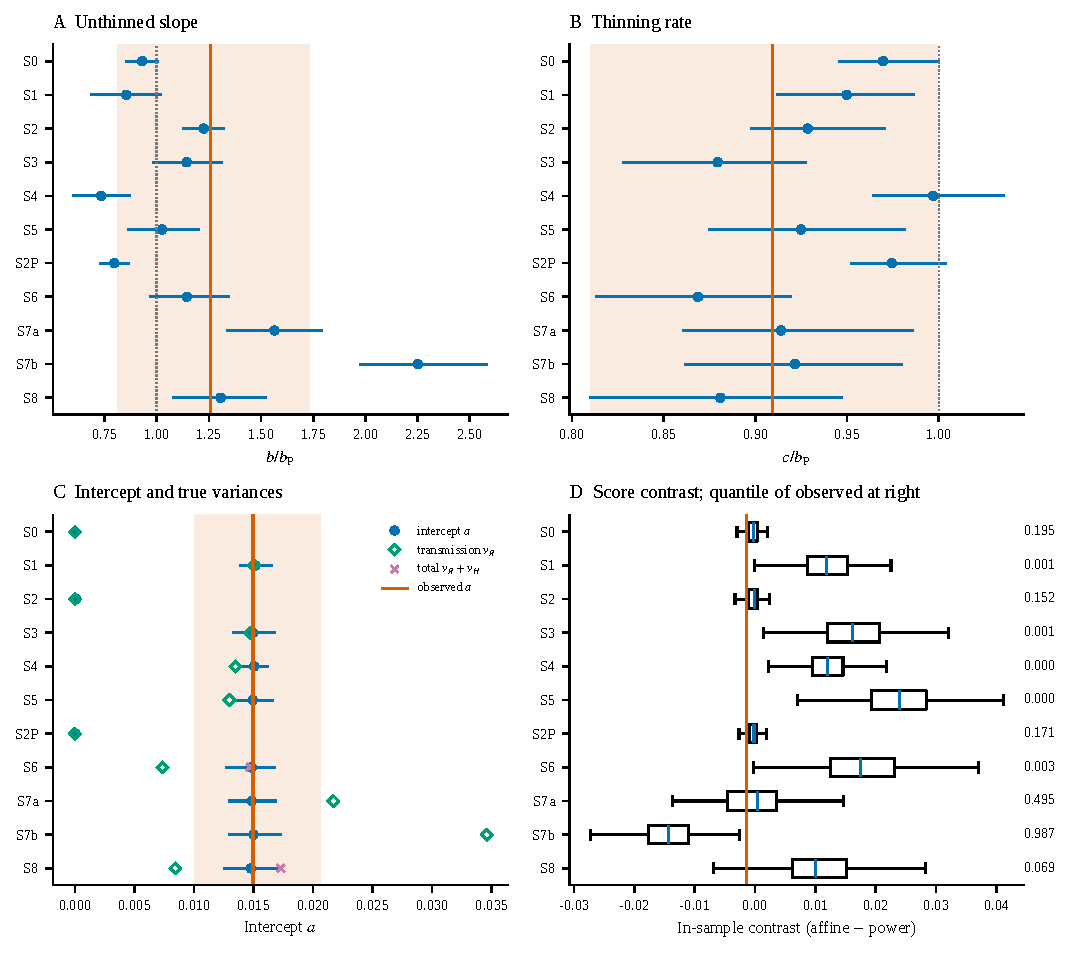
\includegraphics[width=0.95\linewidth]{figures/fig_09_audit.pdf}
\caption{Known-truth audit of the dispersion diagnostics on the real $R_A$ design, with simulated counts aligned to the observed median. Panel A shows the counting slope relative to the independent-Poisson reference, $b/\bP$, by generator. Panel B shows the thinning rate relative to the same reference, $c/\bP$. Panel C shows the fitted intercept $a$ against the true transmission relative variance and the true total, which differ only under S6 and S8. Panel D shows the in-sample score contrast between the affine and power-law fits, with the quantile of the observed value among synthetic panels at the right; boxes span the interquartile range and whiskers 1.5 times it. In panels A--C points are means over 200 panels per generator (100 panels for thinning) and bars are 2.5--97.5\% Monte Carlo ranges. The vertical line and shaded band mark the observed value and its bootstrap 95\% confidence interval; dotted lines mark 1. Generator labels are defined in Table~\ref{tab:ademp}; generator S9 is reported in Tables~\ref{tab:ma_tests} and~\ref{tab:ma_coverage}.}
\label{fig:audit}
\end{figure}

\FloatBarrier
\clearpage
\section{Supplementary tables and figures}
\label{app:supplement}
\renewcommand{\thetable}{S\arabic{table}}
\setcounter{table}{0}
\renewcommand{\thefigure}{S\arabic{figure}}
\setcounter{figure}{0}

Tables~\ref{tab:ma_baselines}--\ref{tab:ma_heldout_sim} give the slope references, the thinning check, the participation adjustment, the within-state slopes, the off-season reporting descriptors and the held-out comparison of curve shapes cited in the main text. Tables~\ref{tab:r2-deciles}--\ref{tab:r2-interval-types} give the decile fits, the state-structured generators, the clamp sensitivity of the wild bootstrap, the pigeonhole bootstrap under fresh-draw generators and the type of every interval quoted in the text. Table~\ref{tab:secondary} also reports the growth-factor statistic $G$ of the original analysis, which the revised analysis does not use, and season-specific fits with separate slopes, which differ from the common-slope season intercepts of Table~\ref{tab:rev_season_effects}.

\FloatBarrier
\begin{table}[htbp]
\centering
\small
\caption{Branching-Poisson and independent-Poisson slope references, analytic, simulated and observed}\label{tab:ma_baselines}
\setlength{\tabcolsep}{2pt}
\begin{tabularx}{\linewidth}{@{}>{\raggedright\arraybackslash}p{0.2400\linewidth}>{\raggedright\arraybackslash}p{0.1400\linewidth}>{\raggedright\arraybackslash}p{0.1400\linewidth}>{\raggedright\arraybackslash}p{0.1400\linewidth}>{\raggedright\arraybackslash}p{0.1400\linewidth}>{\raggedright\arraybackslash}p{0.1400\linewidth}@{}}
\toprule
Reference & Analytic reference / $b_P$ & Simulated b/$b_P$ (no heterogeneity) & MC SE & Simulated / analytic & Observed b / reference \\
\midrule
Branching-Poisson, $\rho$ = 0.1 & 0.944 & 0.877 [0.802, 0.955] & 0.0029 & 0.929 & 1.33 [0.86, 1.84] \\
Branching-Poisson, $\rho$ = 0.25 & 0.861 & 0.802 [0.734, 0.878] & 0.0026 & 0.932 & 1.46 [0.94, 2.02] \\
Branching-Poisson, $\rho$ = 0.5 & 0.722 & 0.669 [0.618, 0.714] & 0.0019 & 0.927 & 1.74 [1.12, 2.41] \\
Branching-Poisson, $\rho$ = 1 & 0.443 & 0.402 [0.373, 0.434] & 0.0012 & 0.907 & 2.84 [1.83, 3.94] \\
Independent-Poisson $b_P$ & 1 & 0.930 [0.853, 1.005] & 0.0029 & 0.930 & 1.26 [0.81, 1.73] \\
\bottomrule
\end{tabularx}
\par\smallskip
\begin{minipage}{\linewidth}\footnotesize\raggedright
The branching-Poisson reference is $b_{P,\mathrm{br}}$($\rho$) = mean over the observed retained rows of $\kappa^2$ [(1 - $\rho$) + ($C_t$ + 0.5)/($C_{t+1}$ + 0.5)]; independent-Poisson reference $b_P$ = 0.4455. Simulated rows use a pure branching chain with Poisson offspring and binomial reporting $\rho$ (independent-Poisson counts, S0, in the last row), no transmission heterogeneity, count-aligned as in the audit. Each has 200 panels, with the Monte Carlo 2.5-97.5\% range in brackets, and simulated / analytic is not normalised by the independent-Poisson row. The observed row uses the primary bootstrap (2,000 draws), with $b_{P,\mathrm{br}}$ recomputed with the weights of each draw. The ratio of the observed slope to the reference depends on the reporting probability.
\end{minipage}
\end{table}

\FloatBarrier
\begin{table}[htbp]
\centering
\small
\caption{Exact expected thinning increment against the delta prediction $b_P$}\label{tab:ma_thinning_exact}
\setlength{\tabcolsep}{2pt}
\begin{tabularx}{\linewidth}{@{}>{\raggedright\arraybackslash}p{0.2400\linewidth}>{\raggedright\arraybackslash}p{0.1400\linewidth}>{\raggedright\arraybackslash}p{0.1400\linewidth}>{\raggedright\arraybackslash}p{0.1400\linewidth}>{\raggedright\arraybackslash}p{0.1400\linewidth}>{\raggedright\arraybackslash}p{0.1400\linewidth}@{}}
\toprule
q & Exact rate & Exact rate / $b_P$ & MC rate [95\% CI] & Leverage in c & Positive-part mass (max) \\
\midrule
0.8 & 0.4672 & 1.049 & 0.4588 [0.3731, 0.5557] & 0.001 & 0.0e+00 \\
0.6 & 0.4845 & 1.087 & 0.4745 [0.4064, 0.5532] & 0.004 & 0.0e+00 \\
0.5 & 0.4957 & 1.113 & 0.4969 [0.4243, 0.5606] & 0.009 & 0.0e+00 \\
0.4 & 0.5050 & 1.133 & 0.4997 [0.4397, 0.5611] & 0.021 & 0.0e+00 \\
0.3 & 0.5051 & 1.134 & 0.5067 [0.4482, 0.5539] & 0.051 & 0.0e+00 \\
0.2 & 0.4798 & 1.077 & 0.4749 [0.4292, 0.5229] & 0.151 & 0.0e+00 \\
0.1 & 0.3836 & 0.861 & 0.3804 [0.3337, 0.4204] & 0.763 & 0.0e+00 \\
c, all q & 0.4084 & 0.917 & 0.4051 [0.3656, 0.4413] & 1.000 & -- \\
c, without q = 0.1 & 0.4882 & 1.096 & -- & -- & -- \\
\bottomrule
\end{tabularx}
\par\smallskip
\begin{minipage}{\linewidth}\footnotesize\raggedright
Rate = ($b_q$ - $b_1$)/(1/q - 1) from the affine FGLS fit of the exact expected thinned loss (binomial supports summed, mass below 1e-13 dropped); $b_P$ = 0.4455 is the delta-method prediction. Leverage is the share of the least-squares rate through the origin carried by each q. As a check, independent-thinning MC gives 0.4903 (SE 0.0048) against an expected-loss value of 0.4957 at q = 0.5, and 0.3832 (SE 0.0024) against 0.3836 at q = 0.1.
\end{minipage}
\end{table}

\FloatBarrier
\begin{table}[!tbp]
\centering
\scriptsize
\setlength{\tabcolsep}{3pt}
\caption{Shared-count binomial thinning of the $R_A$ sample (n=1748): summary by subset}
\label{tab:thinning}
\begin{tabularx}{\linewidth}{@{}ll*{5}{>{\centering\arraybackslash}X}@{}}
\toprule
Subset (n) & Fit over & $\bP$ [95\% CI] & $c$ [95\% CI] & $c/\bP$ [95\% CI] & $\Delta a$ rate $\times10^{3}$ [95\% CI] & $c/\bP$ by $q$, range \\
\midrule
full (1748) & all $q$ & 0.446 [0.428, 0.466] & 0.405 [0.366, 0.441] & 0.909 [0.810, 0.999] & -0.13 [-0.62, 0.47] & 0.85--1.14 \\
 & $q\ge0.2$ &  & 0.485 [0.439, 0.528] & 1.088 [0.994, 1.186] & -0.81 [-1.70, 0.05] & 1.03--1.14 \\
\addlinespace[2pt]
highCt50 (828) & all $q$ & 0.421 [0.403, 0.439] & 0.473 [0.409, 0.550] & 1.126 [0.970, 1.316] & -0.19 [-0.69, 0.15] & 1.05--1.14 \\
 & $q\ge0.2$ &  & 0.459 [0.381, 0.560] & 1.092 [0.903, 1.327] & -0.24 [-0.96, 0.21] & 1.05--1.10 \\
\addlinespace[2pt]
both50 (821) & all $q$ & 0.418 [0.401, 0.436] & 0.493 [0.420, 0.574] & 1.178 [1.004, 1.379] & -0.31 [-0.90, 0.10] & 1.16--1.21 \\
 & $q\ge0.2$ &  & 0.490 [0.397, 0.607] & 1.171 [0.953, 1.462] & -0.43 [-1.33, 0.12] & 1.16--1.21 \\
\bottomrule
\end{tabularx}
\par\smallskip
\begin{minipage}{\linewidth}\footnotesize\raggedright Thinning probabilities $q\in\{0.8, 0.6, 0.5, 0.4, 0.3, 0.2, 0.1\}$. $c$ is the increase of the slope per unit of $1/q-1$ and the $\Delta a$ rate the corresponding change of the intercept; $\bP$ is the independent-Poisson reference (plug-in delta value). highCt50 requires a current count of at least 50 and both50 both adjacent counts of at least 50; eligibility is fixed before thinning. Pairs bootstrap with B=1000 draws, 400 thinning replicates for the point estimate and 50 per bootstrap draw; the Monte Carlo precision criterion (MC SE at most 0.1 times the point estimate on the monitored summaries) is met; point fits 8400/8400, bootstrap fits 1049999/1050000. The last column gives the range of the per-$q$ point estimates of $c/\bP$ over the $q$ values of the fit. Per-$q$ estimates, simultaneous bands over $q$ and leave-one-$q$-out fits are in the released file analysis/authors/thinning.json.\end{minipage}
\end{table}

\FloatBarrier
\begingroup\scriptsize\setlength{\tabcolsep}{2pt}
\begin{longtable}{@{}>{\raggedright\arraybackslash}p{\dimexpr 0.2400\linewidth-3.500pt\relax}>{\raggedright\arraybackslash}p{\dimexpr 0.1000\linewidth-3.500pt\relax}>{\raggedright\arraybackslash}p{\dimexpr 0.1000\linewidth-3.500pt\relax}>{\raggedright\arraybackslash}p{\dimexpr 0.1000\linewidth-3.500pt\relax}>{\raggedright\arraybackslash}p{\dimexpr 0.1000\linewidth-3.500pt\relax}>{\raggedright\arraybackslash}p{\dimexpr 0.1000\linewidth-3.500pt\relax}>{\raggedright\arraybackslash}p{\dimexpr 0.1000\linewidth-3.500pt\relax}>{\raggedright\arraybackslash}p{\dimexpr 0.1000\linewidth-3.500pt\relax}@{}}
\caption{Small-count variance of the log thinned count relative to the delta approximation}\label{tab:ma_varlog}\\
\toprule
C & q = 0.8 & q = 0.6 & q = 0.5 & q = 0.4 & q = 0.3 & q = 0.2 & q = 0.1 \\
\midrule
\endfirsthead
\multicolumn{8}{@{}l}{\textit{(continued)}}\\
\toprule
C & q = 0.8 & q = 0.6 & q = 0.5 & q = 0.4 & q = 0.3 & q = 0.2 & q = 0.1 \\
\midrule
\endhead
\midrule
\multicolumn{8}{r@{}}{\textit{(continued on next page)}}\\
\endfoot
\bottomrule
\endlastfoot
5 & 1.05 & 1.11 & 1.11 & 1.04 & 0.86 & 0.57 & 0.21 \\
10 & 1.02 & 1.05 & 1.08 & 1.12 & 1.13 & 0.99 & 0.53 \\
20 & 1.01 & 1.02 & 1.03 & 1.05 & 1.09 & 1.14 & 0.97 \\
45 & 1.00 & 1.01 & 1.01 & 1.02 & 1.03 & 1.06 & 1.14 \\
100 & 1.00 & 1.00 & 1.01 & 1.01 & 1.01 & 1.02 & 1.06 \\
500 & 1.00 & 1.00 & 1.00 & 1.00 & 1.00 & 1.00 & 1.01 \\
\end{longtable}
\vspace{-.5\baselineskip}
\noindent\begin{minipage}{\linewidth}\footnotesize\raggedright
Exact added variance Var log(Bin(C, q) + 0.5) - Var log(C + 0.5) divided by the delta value (1 - q)/(qC). Values below 1 mean that thinning adds less variance than the delta method assumes.
\end{minipage}\par
\endgroup

\FloatBarrier
\begin{figure}[!tbp]
\centering
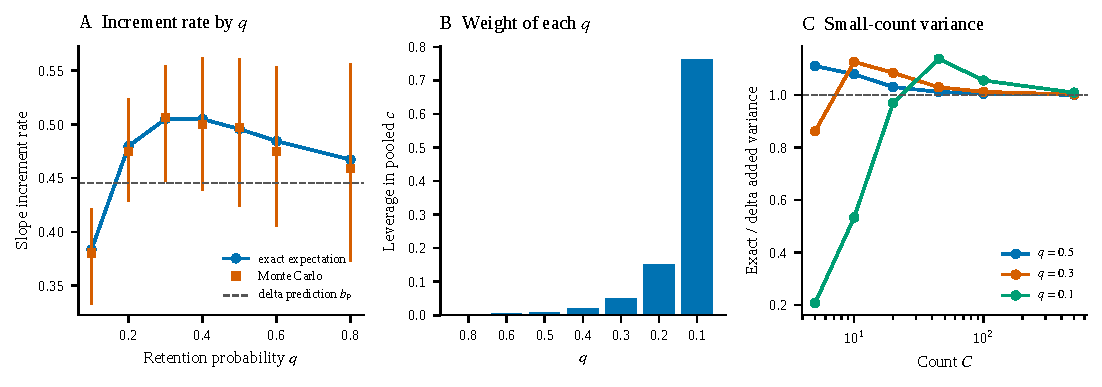
\includegraphics[width=0.98\linewidth]{figures/fig_10_thinning_exact.pdf}
\caption{Exact thinning expectation on the observed counts. Panel A shows the expected increment rate of the inverse-count slope by retention probability $q$, exact expectation against Monte Carlo estimates with 95\% ranges; the dashed line is the delta prediction $\bP=0.4455$. Panel B shows the share of each $q$ in the leverage of the pooled least-squares rate $c$. Panel C shows the exact added variance of the log thinned count relative to its delta approximation, by original count $C$, for three retention probabilities.}
\label{fig:thinning-exact}
\end{figure}
\clearpage
\begingroup\scriptsize\setlength{\tabcolsep}{2pt}
\begin{longtable}{@{}>{\raggedright\arraybackslash}p{\dimexpr 0.2400\linewidth-3.333pt\relax}>{\raggedright\arraybackslash}p{\dimexpr 0.1400\linewidth-3.333pt\relax}>{\raggedright\arraybackslash}p{\dimexpr 0.1400\linewidth-3.333pt\relax}>{\raggedright\arraybackslash}p{\dimexpr 0.1400\linewidth-3.333pt\relax}>{\raggedright\arraybackslash}p{\dimexpr 0.1400\linewidth-3.333pt\relax}>{\raggedright\arraybackslash}p{\dimexpr 0.1400\linewidth-3.333pt\relax}@{}}
\caption{Season-specific fits and reporting participation sensitivity}\label{tab:secondary}\\
\toprule
Statistic / period & n & a / change [95\% CI] & b / original a & b/a / adjusted a & Finite/B \\
\midrule
\endfirsthead
\multicolumn{6}{@{}l}{\textit{(continued)}}\\
\toprule
Statistic / period & n & a / change [95\% CI] & b / original a & b/a / adjusted a & Finite/B \\
\midrule
\endhead
\midrule
\multicolumn{6}{r@{}}{\textit{(continued on next page)}}\\
\endfoot
\bottomrule
\endlastfoot
RA / 2022-23 & 365 & 0.01369 [0.0071, 0.02102] & 0.6967 & 50.91 & 1000/1000 \\
RA / 2023-24 & 499 & 0.006174 [0.002667, 0.01542] & 0.7018 & 113.7 & 1000/1000 \\
RA / 2024-25 & 356 & 0.01268 [0.005687, 0.02276] & 0.5826 & 45.93 & 1000/1000 \\
RA / 2025-26 & 528 & 0.02253 [0.008432, 0.03509] & 0.3533 & 15.68 & 1000/1000 \\
RA / reporting adjustment & 1748 & 0.0002939 [-0.0003183, 0.0008476] & 0.01495 & 0.01466 & 1000/1000 \\
G / 2022-23 & 367 & 0.07179 [0.03786, 0.1162] & 2.702 & 37.64 & 1000/1000 \\
G / 2023-24 & 503 & 0.03046 [0.0118, 0.07462] & 2.382 & 78.2 & 1000/1000 \\
G / 2024-25 & 357 & 0.06469 [0.03191, 0.1278] & 2.082 & 32.19 & 1000/1000 \\
G / 2025-26 & 529 & 0.1383 [0.03715, 0.2252] & 0.7411 & 5.359 & 1000/1000 \\
G / reporting adjustment & 1756 & 0.000373 [-0.003559, 0.003454] & 0.08401 & 0.08364 & 1000/1000 \\
\end{longtable}
\vspace{-.5\baselineskip}
\noindent\begin{minipage}{\linewidth}\footnotesize\raggedright
Season rows report a with its interval and b, b/a as point estimates only. Reporting-adjustment rows use the a column for original-minus-adjusted a [95\% CI], b for original a, and b/a for adjusted a; the original normalizer is fixed. Season b and b/a come from separate per-season fits without a stored bootstrap; season b/a with intervals from a common-slope model are given in the season table. Summer rows are reported in a separate table. All 1,000 draws were finite in every season for RA and G. Season intervals here use 1,000 draws and those of Table~\ref{tab:ma_sensitivity} 2,000, so their limits differ slightly.
\end{minipage}\par
\endgroup

\clearpage
\begingroup\scriptsize\setlength{\tabcolsep}{2pt}
\begin{longtable}{@{}>{\raggedright\arraybackslash}p{\dimexpr 0.2400\linewidth-3.200pt\relax}>{\raggedright\arraybackslash}p{\dimexpr 0.1750\linewidth-3.200pt\relax}>{\raggedright\arraybackslash}p{\dimexpr 0.1750\linewidth-3.200pt\relax}>{\raggedright\arraybackslash}p{\dimexpr 0.1750\linewidth-3.200pt\relax}>{\raggedright\arraybackslash}p{\dimexpr 0.1750\linewidth-3.200pt\relax}@{}}
\caption{Within-state, within-week and two-way slopes against the independent-Poisson reference (bootstrap 95\% confidence interval in brackets)}\label{tab:ma_within}\\
\toprule
Estimator & Slope [95\% CI] & Slope / $b_P$ & Slope / pooled b & Fit status \\
\midrule
\endfirsthead
\multicolumn{5}{@{}l}{\textit{(continued)}}\\
\toprule
Estimator & Slope [95\% CI] & Slope / $b_P$ & Slope / pooled b & Fit status \\
\midrule
\endhead
\midrule
\multicolumn{5}{r@{}}{\textit{(continued on next page)}}\\
\endfoot
\bottomrule
\endlastfoot
Pooled affine slope b & 0.560 [0.362, 0.769] & 1.26 [0.81, 1.73] & -- & -- \\
$b_P$, independent-Poisson reference & 0.446 [0.427, 0.465] & -- & -- & -- \\
State FE, iterated FGLS ($b_w$) & 0.379 [0.107, 0.650] & 0.85 [0.24, 1.47] & 0.68 [0.26, 1.01] & -- \\
State FE, one-step WLS & 0.456 [0.228, 0.682] & 1.02 [0.51, 1.53] & 0.81 [0.57, 0.96] & single step \\
Week FE, one-step WLS & 0.634 [0.420, 0.846] & 1.42 [0.96, 1.89] & 1.13 [0.98, 1.34] & single step \\
State + week FE, one-step WLS & 0.480 [0.208, 0.744] & 1.08 [0.47, 1.66] & 0.86 [0.47, 1.14] & single step \\
State + week FE, damped iterated FGLS & 0.414 [0.040, 0.659] & 0.93 [0.09, 1.48] & 0.74 [0.09, 1.10] & converged, 124 it. \\
\end{longtable}
\vspace{-.5\baselineskip}
\noindent\begin{minipage}{\linewidth}\footnotesize\raggedright
The primary bootstrap uses the state-week weights of the primary stream with 2,000 draws, so the pooled row equals Table~\ref{tab:pooled}; draws whose iterated fit does not converge are dropped (1962 valid for the damped two-way slope). The undamped two-way iteration did not converge after 51 iterations (last values 0.4150, 0.4122); damping 0.5 removes the two-cycle. One-step WLS uses the pooled affine working precision; the iterated estimators re-weight with the fixed-effect fitted means.
\end{minipage}\par
\endgroup

\FloatBarrier
\begin{table}[H]
\centering
\small
\caption{Off-season summer descriptors}\label{tab:summer}
\setlength{\tabcolsep}{2pt}
\begin{tabularx}{\linewidth}{@{}>{\raggedright\arraybackslash}p{0.2400\linewidth}>{\raggedright\arraybackslash}p{0.1750\linewidth}>{\raggedright\arraybackslash}p{0.1750\linewidth}>{\raggedright\arraybackslash}p{0.1750\linewidth}>{\raggedright\arraybackslash}p{0.1750\linewidth}@{}}
\toprule
Period & n & Median count scale & Median participation (\%) & IQR(log G) \\
\midrule
Summer 2023 & 772 & 15.55 & 94.24 & 0.4873 \\
Summer 2024 & 400 & 17.12 & 45.59 & 0.6683 \\
Summer 2025 & 839 & 16.25 & 92.31 & 0.4882 \\
\bottomrule
\end{tabularx}
\par\smallskip
\noindent\begin{minipage}{\linewidth}\footnotesize\raggedright
Descriptive summaries of May-October state-weeks with $D_t$ $\ge$ 5: rows, median count scale $D_t$, median reporting participation (\%) and IQR of log G. No model is fitted, so no interval is given. Reporting was voluntary in the 2024 summer only; that contrast is descriptive, not a causal or independently replicated intervention.
\end{minipage}
\end{table}

\clearpage
\begingroup\scriptsize\setlength{\tabcolsep}{2pt}
\begin{longtable}{@{}>{\raggedright\arraybackslash}p{\dimexpr 0.2400\linewidth-3.500pt\relax}>{\raggedright\arraybackslash}p{\dimexpr 0.1000\linewidth-3.500pt\relax}>{\raggedright\arraybackslash}p{\dimexpr 0.1000\linewidth-3.500pt\relax}>{\raggedright\arraybackslash}p{\dimexpr 0.1000\linewidth-3.500pt\relax}>{\raggedright\arraybackslash}p{\dimexpr 0.1000\linewidth-3.500pt\relax}>{\raggedright\arraybackslash}p{\dimexpr 0.1000\linewidth-3.500pt\relax}>{\raggedright\arraybackslash}p{\dimexpr 0.1000\linewidth-3.500pt\relax}>{\raggedright\arraybackslash}p{\dimexpr 0.1000\linewidth-3.500pt\relax}@{}}
\caption{Held-out comparison of the affine and power loss models with paired uncertainty}\label{tab:ma_validation}\\
\toprule
Held-out unit & Folds & Mean power - affine score & Paired fold SE & z & Folds favouring affine & Bootstrap 95\% CI & Bootstrap share favouring affine \\
\midrule
\endfirsthead
\multicolumn{8}{@{}l}{\textit{(continued)}}\\
\toprule
Held-out unit & Folds & Mean power - affine score & Paired fold SE & z & Folds favouring affine & Bootstrap 95\% CI & Bootstrap share favouring affine \\
\midrule
\endhead
\midrule
\multicolumn{8}{r@{}}{\textit{(continued on next page)}}\\
\endfoot
\bottomrule
\endlastfoot
State & 51 & -0.0020 & 0.0068 & -0.30 & 26/51 & [-0.0290, 0.0298] & 0.43 \\
Season & 4 & 0.0046 & 0.0087 & 0.53 & 3/4 & [-0.0295, 0.0655] & 0.54 \\
\end{longtable}
\vspace{-.5\baselineskip}
\noindent\begin{minipage}{\linewidth}\footnotesize\raggedright
Score: weighted mean of L/mu + log mu on held-out rows; positive differences favour the affine model. Paired fold SE from the between-fold variation of the paired differences; state-week bootstrap with 1000 draws refits both models in every fold.
\end{minipage}\par
\endgroup


\begingroup\let\oldtable\table\renewcommand{\table}[1][]{\oldtable[!h]}
\begin{table}[!tbp]
\centering
\scriptsize
\setlength{\tabcolsep}{3pt}
\caption{Held-out power-minus-affine score contrast on synthetic panels from each generator}
\label{tab:ma_heldout_sim}
\begin{tabularx}{\linewidth}{@{}l*{6}{>{\centering\arraybackslash}X}@{}}
\toprule
 & \multicolumn{3}{c}{Leave one state out (51 folds)} & \multicolumn{3}{c}{Leave one season out (4 folds)} \\
\cmidrule(lr){2-4}\cmidrule(l){5-7}
Generator & Mean contrast ($\times10^{3}$) & Affine better & Observed quantile & Mean contrast ($\times10^{3}$) & Affine better & Observed quantile \\
Observed & -2.02 & & & 4.63 & & \\
\midrule
S0 & -1.01 (0.19) & 0.34 & 0.235 (0.030) & -0.89 (0.23) & 0.38 & 0.970 (0.012) \\
S1 & 12.84 (0.37) & 0.99 & 0.000 (0.000) & 12.97 (0.37) & 0.99 & 0.060 (0.017) \\
S2 & -0.21 (0.13) & 0.51 & 0.125 (0.023) & -0.09 (0.15) & 0.50 & 0.985 (0.009) \\
S2P & -1.00 (0.18) & 0.35 & 0.215 (0.029) & -0.81 (0.31) & 0.42 & 0.980 (0.010) \\
S3 & 17.38 (0.44) & 1.00 & 0.000 (0.000) & 17.49 (0.44) & 1.00 & 0.000 (0.000) \\
S4 & 11.21 (0.36) & 0.99 & 0.000 (0.000) & 15.78 (0.38) & 1.00 & 0.010 (0.007) \\
S5 & 24.03 (0.48) & 1.00 & 0.000 (0.000) & 28.32 (0.58) & 1.00 & 0.000 (0.000) \\
S6 & 18.74 (0.59) & 0.99 & 0.000 (0.000) & 18.60 (0.58) & 0.99 & 0.045 (0.015) \\
S7a & -1.32 (0.44) & 0.41 & 0.475 (0.035) & -0.85 (0.44) & 0.44 & 0.805 (0.028) \\
S7b & -15.42 (0.38) & 0.00 & 0.995 (0.005) & -14.31 (0.40) & 0.01 & 1.000 (0.000) \\
S8 & 11.07 (0.60) & 0.91 & 0.050 (0.015) & 11.15 (0.62) & 0.91 & 0.220 (0.029) \\
S9 & 11.83 (0.59) & 0.92 & 0.055 (0.016) & 12.60 (0.62) & 0.93 & 0.145 (0.025) \\
\bottomrule
\end{tabularx}
\par\smallskip
\begin{minipage}{\linewidth}\footnotesize\raggedright 200 synthetic panels per generator, each analysed with the fold design and score of the data: mean of $L/\mu+\log\mu$ on the held-out rows, weighted by rows, power law minus affine (positive values favour the affine form). Mean contrast with its Monte Carlo standard error; affine better, share of panels with a positive contrast; observed quantile, share of panels with a contrast at or below the observed one, with binomial Monte Carlo standard error.\end{minipage}
\end{table}

\endgroup
\FloatBarrier
\clearpage
\begin{table}[!tbp]
\centering
\scriptsize\renewcommand{\arraystretch}{1.15}
\setlength{\tabcolsep}{3pt}
\caption{Observed and fitted loss by decile of the current-week count}
\label{tab:r2-deciles}
\begin{tabularx}{\linewidth}{@{}rrrrrlrrrr@{}}
\toprule
Decile & $C_t$ & $n$ & Mean $C_t$ & Mean $L$ & 95\% interval & Affine & Power & Three-par. & Affine inside \\
\midrule
1 & 5--10 & 188 & 7.8 & 0.0684 & 0.0538--0.0854 & 0.0906 & 0.0656 & 0.0748 & no \\
2 & 11--15 & 180 & 13.0 & 0.0597 & 0.0425--0.0787 & 0.0584 & 0.0533 & 0.0559 & yes \\
3 & 16--21 & 162 & 18.4 & 0.0557 & 0.0431--0.0699 & 0.0457 & 0.0467 & 0.0469 & yes \\
4 & 22--32 & 176 & 26.7 & 0.0321 & 0.0249--0.0404 & 0.0362 & 0.0405 & 0.0392 & yes \\
5 & 33--45 & 173 & 38.5 & 0.0404 & 0.0310--0.0501 & 0.0296 & 0.0352 & 0.0330 & no \\
6 & 46--73 & 174 & 57.4 & 0.0228 & 0.0174--0.0292 & 0.0249 & 0.0303 & 0.0278 & yes \\
7 & 74--116 & 171 & 93.5 & 0.0223 & 0.0166--0.0287 & 0.0210 & 0.0251 & 0.0229 & yes \\
8 & 117--206 & 174 & 153.4 & 0.0191 & 0.0144--0.0241 & 0.0187 & 0.0208 & 0.0193 & yes \\
9 & 207--388 & 175 & 274.2 & 0.0190 & 0.0132--0.0249 & 0.0171 & 0.0167 & 0.0162 & yes \\
10 & 390--3870 & 175 & 881.9 & 0.0110 & 0.0079--0.0137 & 0.0158 & 0.0115 & 0.0130 & no \\
\bottomrule
\end{tabularx}
\par\smallskip\parbox{\linewidth}{\scriptsize\linespread{1.15}\selectfont Rows of $R_A$ (1,748) split at the deciles of the current-week count $C_t$. Mean $L$: observed mean relative squared deviation; 95\% interval from a calendar-week block bootstrap (1,999 draws). Model columns give the mean prediction in the decile under the affine fit $a+b/C$ ($a=0.0150$, $b=0.560$), the power law $cC^{-\gamma}$ ($\gamma=0.383$) and the three-parameter fit $a+bC^{-\gamma}$ ($a=0.0089$, $\gamma=0.617$). Quasi-deviance: affine -4346.2, power -4348.6, three-parameter -4356.9. Last column: whether the affine prediction lies inside the interval of the observed mean.}
\end{table}

\FloatBarrier
\begin{table}[!tbp]
\centering
\scriptsize\renewcommand{\arraystretch}{1.15}
\setlength{\tabcolsep}{3pt}
\caption{State-realistic fresh-draw generators against four features of the observed panel}
\label{tab:r2-generator}
\begin{tabularx}{\linewidth}{@{}Xlllllrrr@{}}
\toprule
Cell & $\sigma$ & T1 $b/b_P$ & T2 P90 & T3 pooled/within & T4 state CV & $E(\hat a)/v_R$ & SE/SD & Coverage \\
\midrule
SR-pop-c0 & failed & 1.06--1.43 & 367 & 1.07--1.47* & 0.41--0.72 & 1.24 & 2.31 & 1.000 \\
SR-pop-c25 & failed & 1.35--1.89* & 364 & 1.02--1.34* & 0.47--0.78 & 1.26 & 1.79 & 0.990 \\
SR-pop-c50 & failed & 1.67--2.21* & 356 & 1.03--1.31* & 0.52--0.93 & 1.25 & 1.81 & 0.990 \\
SR-fe-c25 & failed & 1.45--1.93* & 364 & 1.04--1.41* & 0.55--0.90 & 1.26 & 1.78 & 0.990 \\
SR-pop-c25-r003 & failed & 1.38--1.84* & 363 & 1.02--1.34* & 0.46--0.76 & 1.27 & 1.80 & 1.000 \\
SR-pop-c25-t50 & 0.161 & 1.29--1.77* & 308* & 1.04--1.39* & 0.47--0.93 & 1.56 & 1.63 & 0.960 \\
Observed & -- & 1.26 & 389 & 1.48 & 0.59 & -- & -- & -- \\
\bottomrule
\end{tabularx}
\par\smallskip\parbox{\linewidth}{\scriptsize\linespread{1.15}\selectfont State-realistic generators (200 panels per cell): transmission field around a smoothed observed trend with state-specific variance (multiplier proportional to the population-dependent intercept, or to the state fixed-effect intercepts for SR-fe), clustered admissions with extra-Poisson parameter $\theta_c$ (c0, c25, c50 $=0, 0.25, 0.5$), reporting probability 0.01 (0.003 for r003), trend exponent 1 (0.5 for t50). $\sigma$: transmission SD scale; ``failed'' when the smoothed trend alone exceeds the transmission target ($\sigma=0$). T1--T4: Monte Carlo 2.5--97.5\% range of $b/b_P$, mean P90 of $C_t$ (band 350--428), range of pooled/within slope ratio and of the between-state CV of intercepts; * the observed value lies outside. Success rule of Amendment 2: all four pass in one cell (outcome: M4/M5 unresolved). Last columns: $E(\hat a)/v_R$, observed SE over Monte Carlo SD of $\hat a$, coverage of $E(\hat a)$ by the two-way interval. Data-informed generator design; no inferential result uses these generators.}
\end{table}

\FloatBarrier
\begin{table}[!tbp]
\centering
\scriptsize\renewcommand{\arraystretch}{1.15}
\setlength{\tabcolsep}{3pt}
\caption{Wild bootstrap of the intercept under alternative loss clamps}
\label{tab:r2-clamp}
\begin{tabularx}{\linewidth}{@{}Xrllll@{}}
\toprule
Variant & Valid draws & $p$ (two-sided) & Min.\ $p$ & Clamped rows (\%) & $t^*$ quantiles \\
\midrule
clamp at $10^{-9}$ & 9,999 & 0.0001 & 0.0001 & 13.5 & $-$0.15 / 1.80 / 3.38 \\
clamp at $10^{-7}$ (primary) & 9,999 & 0.0001 & 0.0001 & 13.5 & $-$0.15 / 1.80 / 3.38 \\
clamp at $10^{-5}$ & 9,999 & 0.0001 & 0.0001 & 13.8 & $-$0.16 / 1.80 / 3.38 \\
clamp at $10^{-3}$ & 9,999 & 0.0001 & 0.0001 & 17.0 & 0.43 / 2.03 / 3.53 \\
no clamp & 3,768 & 0.0003 & 0.0003 & 13.5 & 0.32 / 1.11 / 2.88 \\
exclude draws with any clamped row & 0 & not evaluable & -- & -- & -- \\
\bottomrule
\end{tabularx}
\par\smallskip\parbox{\linewidth}{\scriptsize\linespread{1.15}\selectfont Wild cluster bootstrap-$t$ of the intercept (9,999 draws, calendar-week Webb weights, seed 21); $t_{\mathrm{obs}}=7.36$. Valid: draws with a converged fit. Minimum attainable $p$: $1/(\text{valid}+1)$. Clamped rows: share of bootstrap rows whose loss is at or below the clamp (for no clamp: negative losses, kept). $t^*$: 2.5\%, 50\%, 97.5\% quantiles. Every draw contains at least one clamped row, so the exclusion variant has no draws. Secondary calibration; it does not change the E1 verdict.}
\end{table}

\FloatBarrier
\begin{table}[!tbp]
\centering
\scriptsize\renewcommand{\arraystretch}{1.15}
\setlength{\tabcolsep}{3pt}
\caption{Pigeonhole bootstrap SD of the intercept against the Monte Carlo SD}
\label{tab:r2-bootstrap-sd}
\begin{tabularx}{\linewidth}{@{}Xrrrlrr@{}}
\toprule
Generator & Panels & MC SD ($\times10^3$) & Boot.\ SD ($\times10^3$) & Boot./MC & Sandwich/MC & Coverage \\
\midrule
FD-S1 & 100 & 0.976 & 1.742 & 1.78 (1.47--2.22) & 1.02 & 1.00 \\
FD-S8 & 100 & 1.266 & 2.121 & 1.67 (1.29--2.07) & 0.92 & 0.99 \\
FD-S9-25$^\dagger$ & 100 & 1.300 & 2.148 & 1.65 (1.29--2.05) & 0.94 & 1.00 \\
FD-S9-50$^\dagger$ & 100 & 1.324 & 2.196 & 1.66 (1.28--2.22) & 1.03 & 1.00 \\
FD-S9-75$^\dagger$ & 100 & 1.465 & 2.270 & 1.55 (1.19--1.92) & 1.07 & 0.99 \\
\bottomrule
\end{tabularx}
\par\smallskip\parbox{\linewidth}{\scriptsize\linespread{1.15}\selectfont Pigeonhole (state $\times$ calendar-week) bootstrap, 199 draws per panel, on the first 100 stored panels of each fresh-draw generator (panels regenerated exactly from the stored seeds). MC SD: Monte Carlo SD of $\hat a$ over 200 panels. Ratio range over panels in brackets. Sandwich: two-way SE over MC SD. Coverage: share of panels whose percentile interval covers $E(\hat a)$. $^\dagger$ post hoc law. Reading rule of Amendment 2: conservative if every ratio exceeds 1 (outcome: conservative).}
\end{table}

\FloatBarrier
\begin{table}[!tbp]
\centering
\tiny
\setlength{\tabcolsep}{3pt}
\caption{Type and source of every interval quoted in the manuscript}
\label{tab:r2-interval-types}
\begin{tabularx}{\linewidth}{@{}p{0.11\linewidth}p{0.2\linewidth}lp{0.25\linewidth}X@{}}
\toprule
Location & Quantity & Quoted & Type & Source \\
\midrule
Abstract; Results: count-independent floor & a, pooled affine intercept (primary test) & 0.0109--0.0191 & two-way CGM sandwich (state x calendar week), t with G-1 = 41 df & {\ttfamily\tiny results.\allowbreak{}json.\allowbreak{}revision\_2026\_11.\allowbreak{}E1\_intercept.\allowbreak{}primary.\allowbreak{}inference.\allowbreak{}two\_way.\allowbreak{}a\_ci} \\
Results: count-independent floor & b, counting slope & 0.430--0.690 & two-way CGM sandwich (state x calendar week), t with G-1 = 41 df & {\ttfamily\tiny results.\allowbreak{}json.\allowbreak{}revision\_2026\_11.\allowbreak{}E1\_intercept.\allowbreak{}primary.\allowbreak{}inference.\allowbreak{}two\_way.\allowbreak{}b\_ci} \\
Results: count-independent floor & a, clustering by state only & 0.0125--0.0174 & one-way CGM sandwich by state, t with 50 df & {\ttfamily\tiny results.\allowbreak{}json.\allowbreak{}revision\_2026\_11.\allowbreak{}E1\_intercept.\allowbreak{}primary.\allowbreak{}inference.\allowbreak{}state.\allowbreak{}a\_ci} \\
Results: count-independent floor & a, clustering by calendar week only & 0.0112--0.0188 & one-way CGM sandwich by calendar week, t with 41 df & {\ttfamily\tiny results.\allowbreak{}json.\allowbreak{}revision\_2026\_11.\allowbreak{}E1\_intercept.\allowbreak{}primary.\allowbreak{}inference.\allowbreak{}week.\allowbreak{}a\_ci} \\
Results: count-independent floor & a, block bootstrap & 0.0107--0.0192 & calendar-week block bootstrap percentile (1,999 draws) & {\ttfamily\tiny results.\allowbreak{}json.\allowbreak{}revision\_2026\_11.\allowbreak{}E1\_intercept.\allowbreak{}block\_bootstrap.\allowbreak{}a.\allowbreak{}ci} \\
Results: count-independent floor & a, point estimates over 17 specifications & 0.0117--0.0202 & range of point values (not an interval) & {\ttfamily\tiny results.\allowbreak{}json.\allowbreak{}revision\_2026\_11.\allowbreak{}E1\_intercept.\allowbreak{}sensitivities.\allowbreak{}*.\allowbreak{}a (min and max)} \\
Results: count-independent floor & a at C\_t >= 50 & 0.0088--0.0172 & two-way CGM sandwich (state x calendar week), t with G-1 = 41 df & {\ttfamily\tiny results.\allowbreak{}json.\allowbreak{}revision\_2026\_11.\allowbreak{}E1\_intercept.\allowbreak{}sensitivities.\allowbreak{}S-a3\_floor\_50.\allowbreak{}inference.\allowbreak{}two\_way.\allowbreak{}a\_ci} \\
Results: count-independent floor & a, fixed calendar windows & 0.0092--0.0311 & two-way CGM sandwich (state x calendar week), t with G-1 = 41 df & {\ttfamily\tiny results.\allowbreak{}json.\allowbreak{}revision\_2026\_11.\allowbreak{}E1\_intercept.\allowbreak{}sensitivities.\allowbreak{}S-a4\_calendar\_windows.\allowbreak{}inference.\allowbreak{}two\_way.\allowbreak{}a\_ci} \\
Results: count-independent floor & a, leave-one-week-out point estimates & 0.0136--0.0156 & range of point values (not an interval) & {\ttfamily\tiny results.\allowbreak{}json.\allowbreak{}revision\_2026\_11.\allowbreak{}E1\_intercept.\allowbreak{}sensitivities.\allowbreak{}S-a9\_leave\_one\_week\_out (min and max)} \\
Results: fit of the affine form & mean L, lowest count decile & 0.0538--0.0854 & calendar-week block bootstrap percentile (1,999 draws) & {\ttfamily\tiny results.\allowbreak{}json.\allowbreak{}revision\_2026\_11\_r2.\allowbreak{}B\_floor.\allowbreak{}B1\_deciles.\allowbreak{}rows\allowbreak{}[0].\allowbreak{}mean\_L\_ci} \\
Results: fit of the affine form & mean L, highest count decile & 0.0079--0.0137 & calendar-week block bootstrap percentile (1,999 draws) & {\ttfamily\tiny results.\allowbreak{}json.\allowbreak{}revision\_2026\_11\_r2.\allowbreak{}B\_floor.\allowbreak{}B1\_deciles.\allowbreak{}rows\allowbreak{}[9].\allowbreak{}mean\_L\_ci} \\
Results: fit of the affine form & mean L, fifth count decile & 0.0310--0.0501 & calendar-week block bootstrap percentile (1,999 draws) & {\ttfamily\tiny results.\allowbreak{}json.\allowbreak{}revision\_2026\_11\_r2.\allowbreak{}B\_floor.\allowbreak{}B1\_deciles.\allowbreak{}rows\allowbreak{}[4].\allowbreak{}mean\_L\_ci} \\
Results: fit of the affine form & gamma, three-parameter fit, week bootstrap & 0.355--0.870 & calendar-week block bootstrap percentile (1,999 draws) & {\ttfamily\tiny results.\allowbreak{}json.\allowbreak{}revision\_2026\_11\_r2.\allowbreak{}B\_floor.\allowbreak{}B3\_three\_parameter.\allowbreak{}week\_bootstrap.\allowbreak{}gamma.\allowbreak{}ci} \\
Results: fit of the affine form & gamma, three-parameter fit, state bootstrap & 0.438--0.862 & state bootstrap percentile (states resampled) (999 draws) & {\ttfamily\tiny results.\allowbreak{}json.\allowbreak{}revision\_2026\_11\_r2.\allowbreak{}B\_floor.\allowbreak{}B3\_three\_parameter.\allowbreak{}state\_bootstrap.\allowbreak{}gamma.\allowbreak{}ci} \\
Results: fit of the affine form & a, three-parameter fit, week bootstrap & $-$0.0014 to 0.0137 & calendar-week block bootstrap percentile (1,999 draws) & {\ttfamily\tiny results.\allowbreak{}json.\allowbreak{}revision\_2026\_11\_r2.\allowbreak{}B\_floor.\allowbreak{}B3\_three\_parameter.\allowbreak{}week\_bootstrap.\allowbreak{}a.\allowbreak{}ci} \\
Results: fit of the affine form & a, three-parameter fit, state bootstrap & 0.0034--0.0144 & state bootstrap percentile (states resampled) (999 draws) & {\ttfamily\tiny results.\allowbreak{}json.\allowbreak{}revision\_2026\_11\_r2.\allowbreak{}B\_floor.\allowbreak{}B3\_three\_parameter.\allowbreak{}state\_bootstrap.\allowbreak{}a.\allowbreak{}ci} \\
Results: fit of the affine form & mean L, rows at or above P90 & 0.0078--0.0139 & calendar-week block bootstrap percentile (1,999 draws) & {\ttfamily\tiny results.\allowbreak{}json.\allowbreak{}revision\_2026\_11\_r2.\allowbreak{}B\_floor.\allowbreak{}B4\_model\_free\_floor.\allowbreak{}rows\allowbreak{}[1].\allowbreak{}mean\_L\_ci} \\
Abstract; Results: fit of the affine form & relative RMSE, rows at or above P90 (\%) & 8.8--11.8 & calendar-week block bootstrap percentile (1,999 draws) & {\ttfamily\tiny results.\allowbreak{}json.\allowbreak{}revision\_2026\_11\_r2.\allowbreak{}B\_floor.\allowbreak{}B4\_model\_free\_floor.\allowbreak{}rows\allowbreak{}[1].\allowbreak{}rel\_rmse\_ci} \\
Results: fit of the affine form & floor L - b\_hat/C, P90 & 0.0069--0.0132 & calendar-week block bootstrap percentile (1,999 draws) & {\ttfamily\tiny results.\allowbreak{}json.\allowbreak{}revision\_2026\_11\_r2.\allowbreak{}B\_floor.\allowbreak{}B4\_model\_free\_floor.\allowbreak{}rows\allowbreak{}[1].\allowbreak{}floor\_minus\_bhat\_ci} \\
Results: fit of the affine form & floor relative SD, P90 (\%) & 8.3--11.5 & calendar-week block bootstrap percentile (1,999 draws) & {\ttfamily\tiny results.\allowbreak{}json.\allowbreak{}revision\_2026\_11\_r2.\allowbreak{}B\_floor.\allowbreak{}B4\_model\_free\_floor.\allowbreak{}rows\allowbreak{}[1].\allowbreak{}floor\_rel\_sd\_bhat\_ci} \\
Results: fit of the affine form & floor L - b\_P/C, P90 & 0.0071--0.0132 & calendar-week block bootstrap percentile (1,999 draws) & {\ttfamily\tiny results.\allowbreak{}json.\allowbreak{}revision\_2026\_11\_r2.\allowbreak{}B\_floor.\allowbreak{}B4\_model\_free\_floor.\allowbreak{}rows\allowbreak{}[1].\allowbreak{}floor\_minus\_bP\_ci} \\
Results: fit of the affine form & floor relative SD, P75 (\%) & 9.8--13.2 & calendar-week block bootstrap percentile (1,999 draws) & {\ttfamily\tiny results.\allowbreak{}json.\allowbreak{}revision\_2026\_11\_r2.\allowbreak{}B\_floor.\allowbreak{}B4\_model\_free\_floor.\allowbreak{}rows\allowbreak{}[0].\allowbreak{}floor\_rel\_sd\_bhat\_ci} \\
Results: fit of the affine form & floor relative SD, P95 (\%) & 8.0--11.1 & calendar-week block bootstrap percentile (1,999 draws) & {\ttfamily\tiny results.\allowbreak{}json.\allowbreak{}revision\_2026\_11\_r2.\allowbreak{}B\_floor.\allowbreak{}B4\_model\_free\_floor.\allowbreak{}rows\allowbreak{}[2].\allowbreak{}floor\_rel\_sd\_bhat\_ci} \\
Results: what more cases buy & crossover b/a, two-way & 24.1--58.3 & two-way CGM sandwich (state x calendar week), t with G-1 = 41 df, delta method on the log scale & {\ttfamily\tiny results.\allowbreak{}json.\allowbreak{}revision\_2026\_11.\allowbreak{}E1\_intercept.\allowbreak{}primary.\allowbreak{}inference.\allowbreak{}two\_way.\allowbreak{}b\_over\_a\_ci} \\
Results: what more cases buy & crossover b/a, block bootstrap & 23.4--60.5 & calendar-week block bootstrap percentile (1,999 draws) & {\ttfamily\tiny results.\allowbreak{}json.\allowbreak{}revision\_2026\_11.\allowbreak{}E1\_intercept.\allowbreak{}block\_bootstrap.\allowbreak{}b\_over\_a.\allowbreak{}ci} \\
Results: what more cases buy & crossover b/a over other sensitivity analyses & 25.6--55.5 & range of point values (not an interval) & {\ttfamily\tiny results.\allowbreak{}json.\allowbreak{}revision\_2026\_11.\allowbreak{}E1\_intercept.\allowbreak{}sensitivities.\allowbreak{}*.\allowbreak{}b\_over\_a (min and max)} \\
Results: jurisdiction size & a\_1, population coefficient & $-$0.0085 to $-$0.0023 & two-way CGM sandwich (state x calendar week), t with G-1 = 41 df & {\ttfamily\tiny results.\allowbreak{}json.\allowbreak{}revision\_2026\_11\_r2.\allowbreak{}B\_floor.\allowbreak{}B2\_population.\allowbreak{}primary\_linear.\allowbreak{}a1\_ci\_two\_way\_t41} \\
Abstract; Results: jurisdiction size & ratio a(P90)/a(P10), linear model & 0.408--0.609 & state bootstrap percentile (states resampled) (1,999 draws) & {\ttfamily\tiny results.\allowbreak{}json.\allowbreak{}revision\_2026\_11\_r2.\allowbreak{}B\_floor.\allowbreak{}B2\_population.\allowbreak{}primary\_linear.\allowbreak{}ratio\_ci\_state\_bootstrap} \\
Results: jurisdiction size & ratio a(P90)/a(P10), log link & 0.324--0.595 & state bootstrap percentile (states resampled) (1,999 draws) & {\ttfamily\tiny results.\allowbreak{}json.\allowbreak{}revision\_2026\_11\_r2.\allowbreak{}B\_floor.\allowbreak{}B2\_population.\allowbreak{}secondary\_log\_link.\allowbreak{}theta\_ci\_state\_bootstrap, mapped by exp(theta (z\_P90 - z\_P10))} \\
Results: jurisdiction size & b\_1, slope coefficient on population & $-$0.124 to 0.095 & two-way CGM sandwich (state x calendar week), t with G-1 = 41 df & {\ttfamily\tiny results.\allowbreak{}json.\allowbreak{}revision\_2026\_11\_r2.\allowbreak{}B\_floor.\allowbreak{}B2\_population.\allowbreak{}secondary\_b\_varies.\allowbreak{}b1\_ci\_two\_way\_t41} \\
Results: jurisdiction size & a, smallest-population tertile & 0.0145--0.0233 & two-way CGM sandwich (state x calendar week), t with G-1 = 41 df (t with 16 df) & {\ttfamily\tiny results.\allowbreak{}json.\allowbreak{}revision\_2026\_11\_r2.\allowbreak{}B\_floor.\allowbreak{}B2\_population.\allowbreak{}tertiles\_separate\allowbreak{}[0].\allowbreak{}a\_ci\_two\_way} \\
Results: jurisdiction size & a, middle tertile & 0.0125--0.0264 & two-way CGM sandwich (state x calendar week), t with G-1 = 41 df (t with 16 df) & {\ttfamily\tiny results.\allowbreak{}json.\allowbreak{}revision\_2026\_11\_r2.\allowbreak{}B\_floor.\allowbreak{}B2\_population.\allowbreak{}tertiles\_separate\allowbreak{}[1].\allowbreak{}a\_ci\_two\_way} \\
Results: jurisdiction size & a, largest-population tertile & 0.0090--0.0180 & two-way CGM sandwich (state x calendar week), t with G-1 = 41 df (t with 16 df) & {\ttfamily\tiny results.\allowbreak{}json.\allowbreak{}revision\_2026\_11\_r2.\allowbreak{}B\_floor.\allowbreak{}B2\_population.\allowbreak{}tertiles\_separate\allowbreak{}[2].\allowbreak{}a\_ci\_two\_way} \\
Results: jurisdiction size & ratio tertile 3 / tertile 1, common slope & 0.421--0.818 & state bootstrap percentile (states resampled) (999 draws) & {\ttfamily\tiny results.\allowbreak{}json.\allowbreak{}revision\_2026\_11\_r2.\allowbreak{}B\_floor.\allowbreak{}B2\_population.\allowbreak{}tertiles\_common\_slope.\allowbreak{}ratio\_ci\_state\_bootstrap} \\
Results: what the floor contains & a after week centring (leave-state-out) & 0.0078--0.0126 & calendar-week block bootstrap percentile (1,999 draws) & {\ttfamily\tiny results.\allowbreak{}json.\allowbreak{}revision\_2026\_11.\allowbreak{}E3\_within\_week.\allowbreak{}week\_leave\_state\_out.\allowbreak{}a\_boot.\allowbreak{}ci} \\
Results: what the floor contains & reduction of a, leave-state-out week centre (\%) & 10.2--47.8 & calendar-week block bootstrap percentile (1,999 draws) & {\ttfamily\tiny results.\allowbreak{}json.\allowbreak{}revision\_2026\_11.\allowbreak{}E3\_within\_week.\allowbreak{}week\_leave\_state\_out.\allowbreak{}reduction\_vs\_pooled.\allowbreak{}ci} \\
Results: what the floor contains & reduction of a, week centre incl. own row (\%) & 13.8--49.8 & calendar-week block bootstrap percentile (1,999 draws) & {\ttfamily\tiny results.\allowbreak{}json.\allowbreak{}revision\_2026\_11.\allowbreak{}E3\_within\_week.\allowbreak{}week.\allowbreak{}reduction\_vs\_pooled.\allowbreak{}ci} \\
Results: what the floor contains & reduction of a, week centre and scale (\%) & 22.0--57.0 & calendar-week block bootstrap percentile (1,999 draws) & {\ttfamily\tiny results.\allowbreak{}json.\allowbreak{}revision\_2026\_11.\allowbreak{}E3\_within\_week.\allowbreak{}week\_review.\allowbreak{}reduction\_vs\_pooled.\allowbreak{}ci} \\
Results: what the floor contains & reduction of a, season centring (\%) & $-$6.8 to 19.1 & calendar-week block bootstrap percentile (1,999 draws) & {\ttfamily\tiny results.\allowbreak{}json.\allowbreak{}revision\_2026\_11.\allowbreak{}E3\_within\_week.\allowbreak{}season.\allowbreak{}reduction\_vs\_pooled.\allowbreak{}ci} \\
Results: what the floor contains & implied transmission SD over 71 mechanisms (\%) & 8.6--18.6 & range of point values (not an interval) & {\ttfamily\tiny results.\allowbreak{}json.\allowbreak{}revision\_2026\_11.\allowbreak{}implied\_sd\_grid.\allowbreak{}envelope\_all.\allowbreak{}point\_range} \\
Results: what the floor contains & implied transmission SD, propagated (\%) & 6.9--22.7 & propagated envelope: two-way interval of a combined with MC 2.5-97.5\% range of r & {\ttfamily\tiny results.\allowbreak{}json.\allowbreak{}revision\_2026\_11.\allowbreak{}implied\_sd\_grid.\allowbreak{}envelope\_all.\allowbreak{}interval\_envelope} \\
Results: what the floor contains & implied SD, 13 slope-reproducing mechanisms (\%) & 8.6--13.9 & range of point values (not an interval) & {\ttfamily\tiny results.\allowbreak{}json.\allowbreak{}revision\_2026\_11.\allowbreak{}implied\_sd\_grid.\allowbreak{}envelope\_reproducing\_counting\_slope.\allowbreak{}point\_range} \\
Results: what the floor contains & intercept recovery, daily renewal (\%) & 75--78 & range of Monte Carlo summaries over generators or cells (not an interval) & {\ttfamily\tiny results.\allowbreak{}json.\allowbreak{}revision\_2026\_11.\allowbreak{}daily\_renewal.\allowbreak{}SC1\_one\_generation\_map\_carries\_over.\allowbreak{}range} \\
Results: intercept and its sources & relative bias of a, FD-S1 (\%) & 0.5--2.3 & panel bootstrap percentile over simulated panels (2,000 draws) & {\ttfamily\tiny results.\allowbreak{}json.\allowbreak{}revision\_2026\_11\_r2.\allowbreak{}C\_total\_bias.\allowbreak{}generators.\allowbreak{}FD-S1.\allowbreak{}relative\_bias\_ci} \\
Results: intercept and its sources & relative bias of a, FD-S8 (\%) & $-$15.1 to $-$13.3 & panel bootstrap percentile over simulated panels (2,000 draws) & {\ttfamily\tiny results.\allowbreak{}json.\allowbreak{}revision\_2026\_11\_r2.\allowbreak{}C\_total\_bias.\allowbreak{}generators.\allowbreak{}FD-S8.\allowbreak{}relative\_bias\_ci} \\
Results: intercept and its sources & relative bias of a, FD-S9 variants (\%) & $-$14.9 to $-$13.8 & range of point values (not an interval) & {\ttfamily\tiny results.\allowbreak{}json.\allowbreak{}revision\_2026\_11\_r2.\allowbreak{}C\_total\_bias.\allowbreak{}generators.\allowbreak{}FD-S9-*.\allowbreak{}relative\_bias (min and max)} \\
Abstract; Results: intercept and its sources & shortfall against the total with reporting shocks (\%) & 6.3--22.1 & range of point values (not an interval) & {\ttfamily\tiny results.\allowbreak{}json.\allowbreak{}revision\_2026\_11\_r2.\allowbreak{}C\_total\_bias.\allowbreak{}generators.\allowbreak{}*.\allowbreak{}relative\_bias (min and max over generators\_with\_reporting\_shock)} \\
Results: intercept and its sources & w\_H over laws & 0.10--0.91 & range of point values (not an interval) & {\ttfamily\tiny results.\allowbreak{}json.\allowbreak{}revision\_2026\_11\_r2.\allowbreak{}C\_total\_bias.\allowbreak{}generators.\allowbreak{}*.\allowbreak{}w\_H (min and max)} \\
Results: intercept and its sources & mechanism-conditional rescaled a & 0.0160--0.0192 & range of point values (not an interval) & {\ttfamily\tiny results.\allowbreak{}json.\allowbreak{}revision\_2026\_11\_r2.\allowbreak{}C\_total\_bias.\allowbreak{}mechanism\_conditional\_rescaling.\allowbreak{}a\_obs\_over\_t\_g\_range} \\
Results: external reporting data & change in a after participation adjustment & $-$0.00086 to 0.00027 & calendar-week block bootstrap percentile (1,999 draws) & {\ttfamily\tiny results.\allowbreak{}json.\allowbreak{}revision\_2026\_11\_r2.\allowbreak{}D2\_reporting\_data.\allowbreak{}coverage\_adjustment.\allowbreak{}difference\_ci\_week\_bootstrap} \\
Results: external reporting data & a, first-issue counts & 0.0133--0.0298 & calendar-week block bootstrap percentile (1,999 draws) & {\ttfamily\tiny results.\allowbreak{}json.\allowbreak{}revision\_2026\_11\_r2.\allowbreak{}D2\_reporting\_data.\allowbreak{}backfill.\allowbreak{}a\_first\_ci\_week\_bootstrap} \\
Results: external reporting data & a, latest-issue counts & 0.0096--0.0183 & calendar-week block bootstrap percentile (1,999 draws) & {\ttfamily\tiny results.\allowbreak{}json.\allowbreak{}revision\_2026\_11\_r2.\allowbreak{}D2\_reporting\_data.\allowbreak{}backfill.\allowbreak{}a\_latest\_ci\_week\_bootstrap} \\
Results: external reporting data & a, first minus latest & 0.0016--0.0146 & calendar-week block bootstrap percentile (1,999 draws) & {\ttfamily\tiny results.\allowbreak{}json.\allowbreak{}revision\_2026\_11\_r2.\allowbreak{}D2\_reporting\_data.\allowbreak{}backfill.\allowbreak{}a\_first\_minus\_latest\_ci\_week\_bootstrap} \\
Results: counting slope & b/b\_P, plug-in reference & 0.97--1.59 & calendar-week block bootstrap percentile (1,999 draws) & {\ttfamily\tiny results.\allowbreak{}json.\allowbreak{}revision\_2026\_11.\allowbreak{}E1\_intercept.\allowbreak{}block\_bootstrap.\allowbreak{}b\_over\_bP.\allowbreak{}ci} \\
Results: counting slope & b/b\_P, normalised plug-in reference & 1.02--1.64 & two-way CGM sandwich (state x calendar week), t with G-1 = 41 df, reference fixed & {\ttfamily\tiny results.\allowbreak{}json.\allowbreak{}revision\_2026\_11\_r2.\allowbreak{}F2\_poisson\_reference.\allowbreak{}b\_over\_bP\_ci\_two\_way\_bP\_fixed.\allowbreak{}normalised\_plugin} \\
Results: counting slope & b/b\_P, simulated exact reference & 1.08--1.73 & two-way CGM sandwich (state x calendar week), t with G-1 = 41 df, reference fixed & {\ttfamily\tiny results.\allowbreak{}json.\allowbreak{}revision\_2026\_11\_r2.\allowbreak{}F2\_poisson\_reference.\allowbreak{}b\_over\_bP\_ci\_two\_way\_bP\_fixed.\allowbreak{}simulated\_exact} \\
Results: counting slope & b/b\_P, state fixed effects & 0.24--1.47 & state x calendar-week pigeonhole bootstrap percentile (2,000 draws) & {\ttfamily\tiny ma\_extensions.\allowbreak{}json.\allowbreak{}within.\allowbreak{}over\_bP.\allowbreak{}state\_authors.\allowbreak{}ci95} \\
Results: counting slope & b/b\_P, week fixed effects & 0.96--1.89 & state x calendar-week pigeonhole bootstrap percentile (2,000 draws) & {\ttfamily\tiny ma\_extensions.\allowbreak{}json.\allowbreak{}within.\allowbreak{}over\_bP.\allowbreak{}week\_onestep.\allowbreak{}ci95} \\
Results: counting slope & expected b/b\_P for rho <= 0.01 & 0.85--0.91 & range of Monte Carlo summaries over generators or cells (not an interval) & {\ttfamily\tiny results.\allowbreak{}json.\allowbreak{}revision\_2026\_11.\allowbreak{}rho\_k\_grid.\allowbreak{}SC3\_b\_over\_bP\_0.\allowbreak{}9\_1.\allowbreak{}1\_at\_rho\_le\_0.\allowbreak{}01.\allowbreak{}range} \\
Results: season intercepts & 2023-24 intercept & 0.0050--0.0100 & two-way CGM sandwich (state x calendar week), t with G-1 = 41 df, delta method on the log scale & {\ttfamily\tiny results.\allowbreak{}json.\allowbreak{}revision\_2026\_11.\allowbreak{}season\_test.\allowbreak{}effects.\allowbreak{}seasons.\allowbreak{}2023-24.\allowbreak{}ci\_sandwich\_log\_delta} \\
Results: season intercepts & other-season intercepts & 0.0154--0.0180 & range of point values (not an interval) & {\ttfamily\tiny results.\allowbreak{}json.\allowbreak{}revision\_2026\_11.\allowbreak{}season\_test.\allowbreak{}effects.\allowbreak{}seasons.\allowbreak{}*.\allowbreak{}a\_s (min and max over 2022-23, 2024-25, 2025-26)} \\
Results: season intercepts & highest / lowest season intercept & 1.75--4.35 & calendar-week block bootstrap percentile within seasons (1,999 draws) & {\ttfamily\tiny results.\allowbreak{}json.\allowbreak{}revision\_2026\_11.\allowbreak{}season\_test.\allowbreak{}effects.\allowbreak{}max\_over\_min.\allowbreak{}ci\_bootstrap} \\
Results: season intercepts & 2023-24 versus other seasons, ratio & 0.29--0.65 & two-way CGM sandwich (state x calendar week), t with G-1 = 41 df, log scale & {\ttfamily\tiny results.\allowbreak{}json.\allowbreak{}revision\_2026\_11.\allowbreak{}season\_test.\allowbreak{}effects.\allowbreak{}post\_hoc\_contrast\_2023\_24\_vs\_mean\_of\_others\_log.\allowbreak{}ci\_sandwich} \\
Results: validity of the intervals & coverage of E(a\_hat), fresh-draw generators & 0.920--0.975 & range of Monte Carlo summaries over generators or cells (not an interval) & {\ttfamily\tiny results.\allowbreak{}json.\allowbreak{}revision\_2026\_11.\allowbreak{}fresh\_draw\_generators.\allowbreak{}generators.\allowbreak{}* (min and max over generators)} \\
Results: validity of the intervals & SE / MC SD, fresh-draw generators & 0.92--1.07 & range of Monte Carlo summaries over generators or cells (not an interval) & {\ttfamily\tiny results.\allowbreak{}json.\allowbreak{}revision\_2026\_11.\allowbreak{}fresh\_draw\_generators.\allowbreak{}generators.\allowbreak{}* (min and max over generators)} \\
Results: validity of the intervals & coverage of the true total, shock generators & 0.44--0.59 & range of Monte Carlo summaries over generators or cells (not an interval) & {\ttfamily\tiny results.\allowbreak{}json.\allowbreak{}revision\_2026\_11.\allowbreak{}fresh\_draw\_generators.\allowbreak{}generators.\allowbreak{}* (min and max over shock generators)} \\
Results: validity of the intervals & observed SE / MC SD, fresh-draw laws of the plan & 1.53--2.08 & range of Monte Carlo summaries over generators or cells (not an interval) & {\ttfamily\tiny results.\allowbreak{}json.\allowbreak{}revision\_2026\_11.\allowbreak{}fresh\_draw\_generators.\allowbreak{}mc\_sd\_over\_observed\_se (reciprocals, FD-S1 to FD-S9-50)} \\
Results: validity of the intervals; Appendix: audit intervals & pigeonhole bootstrap SD / MC SD, fresh-draw generators & 1.55--1.78 & range of Monte Carlo summaries over generators or cells (not an interval) & {\ttfamily\tiny results.\allowbreak{}json.\allowbreak{}revision\_2026\_11\_r2.\allowbreak{}F1\_bootstrap\_sd.\allowbreak{}rule.\allowbreak{}ratios (min and max)} \\
Appendix: audit intervals & pigeonhole bootstrap SD / MC SD, range over panels & 1.19--2.22 & range over simulated panels (not an interval) & {\ttfamily\tiny results.\allowbreak{}json.\allowbreak{}revision\_2026\_11\_r2.\allowbreak{}F1\_bootstrap\_sd.\allowbreak{}generators.\allowbreak{}* (min and max of the per-panel ratio ranges)} \\
Results: validity of the intervals & coverage of E(a\_hat), state-realistic cells & 0.96--1.00 & range of Monte Carlo summaries over generators or cells (not an interval) & {\ttfamily\tiny results.\allowbreak{}json.\allowbreak{}revision\_2026\_11\_r2.\allowbreak{}D1\_state\_realistic\_generators.\allowbreak{}cells.\allowbreak{}*.\allowbreak{}coverage\_of\_E\_a.\allowbreak{}coverage (min and max)} \\
Results: validity of the intervals & observed SE / MC SD, state-realistic cells & 1.63--2.31 & range of Monte Carlo summaries over generators or cells (not an interval) & {\ttfamily\tiny results.\allowbreak{}json.\allowbreak{}revision\_2026\_11\_r2.\allowbreak{}D1\_state\_realistic\_generators.\allowbreak{}cells.\allowbreak{}*.\allowbreak{}sd\_ratio\_observed\_se\_over\_mc\_sd (min and max)} \\
Results: validity of the intervals & E(a\_hat) / simulated total, state-realistic cells (\%) & 70--78 & range of Monte Carlo summaries over generators or cells (not an interval) & {\ttfamily\tiny results.\allowbreak{}json.\allowbreak{}revision\_2026\_11\_r2.\allowbreak{}D1\_state\_realistic\_generators.\allowbreak{}cells.\allowbreak{}*.\allowbreak{}a\_over\_total (min and max)} \\
Results: validity of the intervals & coverage of the true total, state-realistic cells & 0.015--0.16 & range of Monte Carlo summaries over generators or cells (not an interval) & {\ttfamily\tiny results.\allowbreak{}json.\allowbreak{}revision\_2026\_11\_r2.\allowbreak{}D1\_state\_realistic\_generators.\allowbreak{}cells.\allowbreak{}*.\allowbreak{}coverage\_of\_true\_total.\allowbreak{}coverage (min and max)} \\
\bottomrule
\end{tabularx}
\par\smallskip\parbox{\linewidth}{\scriptsize\linespread{1.15}\selectfont 73 intervals and ranges quoted in the abstract, Results and Discussion; source found mechanically in the analysis outputs for 73 (stored pair matching the quoted limits at the quoted precision); the others are ranges assembled from several stored values (path pattern given). CGM: Cameron--Gelbach--Miller. All intervals 95\%.}
\end{table}

\FloatBarrier


% unsrtnat-noid: local copy of unsrtnat without the unused \doi preamble; references numbered by order of first citation
% Keep the bibliography in the manuscript's current column mode unless an
% external publisher template explicitly requires otherwise.
% Keep this exact boundary after the final body input: drain every queued float,
% then start References on a new page. Figures/tables and references never share
% a page, even when the preceding body page has unused space.
\FloatBarrier
\clearpage
\bibliographystyle{unsrtnat-noid}
\bibliography{bibliography}

\end{document}
